%%%%%%%%%%%%%%%%%%%%%%%%%%%%%%%%%%%%%%%%%%%%%%%%%%%%%%%%%%%%%%%%%%%%%%%%%%%%%%%%
% Preámbulo                                                                    %
%%%%%%%%%%%%%%%%%%%%%%%%%%%%%%%%%%%%%%%%%%%%%%%%%%%%%%%%%%%%%%%%%%%%%%%%%%%%%%%%

\documentclass[11pt,a4paper,titlepage,twoside,openright,openbib]{report}

%%% RELACIÓN DE VARIABLES A PERSONALIZAR %%%
%\def\lingua{gal}
\def\lingua{esp} % descomenta esta liña se redactarás a memoria en español
%\def\lingua{eng} % descomenta esta liña se redactarás a memoria en inglés
\def\nome{Diego Trabazo Sardón}                             % substitúe aquí o teu nome
\def\nomedirectorA{José Carlos Dafonte Vázquez}             % substitúe aquí o nome de quen dirixe
\def\titulo{Sistema para la extracción automática de información estructurada a partir de documentos con
elementos de maquetación comunes} % substitúe aquí o título do teu TFG
%\def\mencion{NOME DA MENCIÓN}                        % descomenta a mención correspondente
\def\mencion{COMPUTACIÓN}
%\def\mencion{ENXEÑARÍA DO SOFTWARE}
%\def\mencion{ENXEÑARÍA DE COMPUTADORES}
%\def\mencion{SISTEMAS DE INFORMACIÓN}
%\def\mencion{TECNOLOXÍAS DA INFORMACIÓN}

\def\renomearcadros{si} % descomenta esta liña se redactas a memoria en español e prefires que
                         % os "cuadros" e o "índice de cuadros" se renomeen
                         % a "tablas" e "índice de tablas" respectivamente

\usepackage{estilo_tfg}

% Cambia el tipo y tamaño de la fuente monoespaciada en todo el documento
\setmonofont[Scale=MatchLowercase]{IBMPlexMono}

% Lista de paquetes potencialmente interesantes (uso baixo demanda)

% \usepackage{alltt}       % proporciona o entorno alltt, semellante a verbatim pero que respecta comandos
% \usepackage{enumitem}    % permite personalizar os entornos de lista
% \usepackage{eurofont}    % proporciona o comando \euro
% \usepackage{float}       % permite máis opcións para controlar obxectos flotantes (táboas, figuras)
% \usepackage{hhline}      % permie personalizar as liñas horizontais en arrays e táboas
% \usepackage{longtable}   % permite construir táboas que ocupan máis dunha páxina
% \usepackage{lscape}      % permite colocar partes do documento en orientación apaisada
% \usepackage{moreverb}    % permite personalizar o entorno verbatim
% \usepackage{multirow}    % permite crear celdas que ocupan varias filas da mesma táboa
% \usepackage{pdfpages}    % permite insertar ficheiros en PDF no documento
% \usepackage{rotating}    % permite diferentes tipos de rotacións para figuras e táboas
% \usepackage{subcaption}  % permite a inclusión de varias subfiguras nunha figura
% \usepackage{tabu}        % permite táboas flexibles
% \usepackage{tabularx}    % permite táboas con columnas de anchura determinada
\usepackage{xcolor}
\usepackage{wrapfig}
\usepackage{url}

\definecolor{codegreen}{rgb}{0,0.6,0}
\definecolor{codegray}{rgb}{0.5,0.5,0.5}
\definecolor{codepurple}{rgb}{0.58,0,0.82}
\definecolor{backcolour}{rgb}{0.95,0.95,0.92}

\lstdefinestyle{mystyle}{
    backgroundcolor=\color{backcolour},   
    commentstyle=\color{codegreen},
    keywordstyle=\color{magenta},
    numberstyle=\tiny\color{codegray},
    stringstyle=\color{codepurple},
    basicstyle=\ttfamily\footnotesize,
    breakatwhitespace=false,         
    breaklines=true,                 
    captionpos=b,                    
    keepspaces=true,                 
    numbers=left,                    
    numbersep=5pt,                  
    showspaces=false,                
    showstringspaces=false,
    showtabs=false,                  
    tabsize=2,
    frame=none
}

\lstset{style=mystyle}

%%%%%%%%%%%%%%%%%%%%%%%%%%%%%%%%%%%%%%%%%%%%%%%%%%%%%%%%%%%%%%%%%%%%%%%%%%%%%%%%
% Corpo                                                                        %
%%%%%%%%%%%%%%%%%%%%%%%%%%%%%%%%%%%%%%%%%%%%%%%%%%%%%%%%%%%%%%%%%%%%%%%%%%%%%%%%

\begin{document}

 %%%%%%%%%%%%%%%%%%%%%%%%%%%%%%%%%%%%%%%%
 % Preliminares do documento            %
 %%%%%%%%%%%%%%%%%%%%%%%%%%%%%%%%%%%%%%%%

 \begin{titlepage}
  
  \hspace*{128pt}
  \textcolor{udcpink}{{\fontencoding{T1}\fontfamily{phv}\selectfont Facultade de Informática}}\\[-32pt]

  \begin{center}
    
\includegraphics[scale=0.3]{imaxes/udc}\\[35pt]

    {\large TRABALLO FIN DE GRAO \\
            GRAO EN ENXEÑARÍA INFORMÁTICA \\
            MENCIÓN EN \mencion } \\[100pt]
    
    \begin{huge}
      \begin{spacing}{1.3}
        \bfseries \titulo
      \end{spacing}
    \end{huge}
  \end{center}
  
  \vfill
  
  \begin{flushright}
    {\large
    \begin{tabular}{ll}
      {\bf Estudante:} & \nome \\
      {\bf Dirección:} & \nomedirectora1 \\ % COPIA E PEGA ESTA LIÑA SE O PRECISAS
    \end{tabular}}
  \end{flushright}
  \rightline{A Coruña, \datasimple\today.}
\end{titlepage}

 \paxinaenbranco
 \dedicatoria{Dedicatoria} % escribe neste comando o teu texto de dedicatoria
 \paxinaenbranco
 \paxinaenbranco
 \begin{agradecementos}
 \blindtext                % substitúe este comando polo teu texto de agradecementos
 \end{agradecementos}
 \paxinaenbranco
 %%%%%%%%%%%%%%%%%%%%%%%%%%%%%%%%%%%%%%%%%%%%%%%%%%%%%%%%%%%%%%%%%%%%%%%%%%%%%%%%

\begin{abstract}\thispagestyle{empty}

Este TFG tiene por objetivo la creación de una solución de entorno servidor, para automatizar la adquisición de información desde fuentes de datos semiestructuradas, como son los PDF. El proyecto se enmarca en el ámbito de la transición de organizaciones, públicas o privadas, hacia la informatización de los procesos.
Se centra específicamente en documentos donde existe un modelo común de maquetación, que los representan. Tanto si los ficheros PDF han sido creados digitalmente, por ejemplo, por un sistema de facturación, como si son simplemente producidos a partir de imágenes obtenidas por un escáner, desde documentos en papel, no resulta trivial recuperar de forma eficaz, la información contenida en ellos. El sistema realiza la extracción de la información, construye una representación interna de la misma gracias a sus coordenadas físicas, y posteriormente, la transforma a un formato estructurado, por medio de técnicas de procesamiento de lenguajes formales, en particular mediante los analizadores Flex y GNU Bison.

  \vspace*{25pt}
  \begin{segundoresumo}
This Bachelor's Degree Final Project aims to create a backend solution for automating information acquisition from semi-structured sources, like PDF file format. The project is framed within the scope of easing the transition of public or private organizations towards more process informatization.
It is specifically centered in the case of documents where there is a common layout that represents them. Whether the PDF files were digitally created, for example, by a billing system or they are simply sourced from images produced by a scanner, from paper documents, it is not trivial to effectively get back the information they hold. The system performs the information extraction, builds an internal representation thanks to the data's physical coordinates and finally, transforms that representation to an structured format, by employing formal languages processing techniques, particularly leaning on Flex and GNU Bison anylizers.
  \end{segundoresumo}

\newpage
\vspace*{25pt}
\begin{multicols}{2}
\begin{description}
\item [\palabraschaveprincipal:] \mbox{} \\[-20pt]
  \begin{itemize}
      \item Oficina sin papel 
      \item Lenguajes formales
      \item Flex
      \item Bison
      \item Transformada de Hough
      \item Procesamiento de Lenguajes
  \end{itemize}
%  \blindlist{itemize}[7] % substitúe este comando por un itemize
                         % que relacione as palabras chave
                         % que mellor identifiquen o teu TFG
                         % no idioma principal da memoria (tipicamente: galego)
\end{description}
\begin{description}
\item [\palabraschavesecundaria:] \mbox{} \\[-20pt]
  \begin{itemize}
      \item Paperless Office
      \item Formal languages
      \item Flex
      \item Bison
      \item Hough Transform
  \end{itemize}

  %\blindlist{itemize}[7] % substitúe este comando por un itemize
                         % que relacione as palabras chave
                         % que mellor identifiquen o teu TFG
                         % no idioma secundario da memoria (tipicamente: inglés)
\end{description}
\end{multicols}

\end{abstract}

%%%%%%%%%%%%%%%%%%%%%%%%%%%%%%%%%%%%%%%%%%%%%%%%%%%%%%%%%%%%%%%%%%%%%%%%%%%%%%%%

 \paxinaenbranco

 \pagenumbering{roman}
 \setcounter{page}{1}
 \bstctlcite{IEEEexample:BSTcontrol}

 \tableofcontents
 \listoffigures
 \listoftables
 \lstlistoflistings
 \cleardoublepage

 \pagenumbering{arabic}
 \setcounter{page}{1}

 %%%%%%%%%%%%%%%%%%%%%%%%%%%%%%%%%%%%%%%%
 % Capítulos                            %
 %%%%%%%%%%%%%%%%%%%%%%%%%%%%%%%%%%%%%%%%

 %%%%                 %%%%
%%%% INTRODUCCIÓN    %%%%
%%%%                 %%%%

% TODO explicar que se esperaba colaboración con otra persona del laboratorio Lia2 para la elaboración de una interfaz gráfica para este proyecto.

\chapter{Introducción}
\label{chap:introduccion}

\lettrine{A}{unque} las empresas realizan un esfuerzo por sumarse a la digitalización, sigue siendo habitual que no existan canales de comunicación estandarizados para el intercambio de información con clientes, proveedores o trabajadores. El modelo tradicional se basa en la utilización de documentos en papel como base para dejar evidencia de las operaciones ocurridas. Suponiendo, por ejemplo, un escenario donde una empresa realiza una compra a un proveedor, para completar la entrega del producto, se utiliza un albarán que el transportista presenta en la empresa y se lleva firmado tras el depósito de la mercancía. El cliente se queda con una copia del documento y la operación finaliza o pasa a una siguiente fase, como puede ser el pago de la mercancía. ¿Pero, qué sucede luego con estos documentos? Deben ser archivados como prueba del intercambio y la información tiene que estar disponible en las aplicaciones empresariales de la organización para llevar el control de gastos, nivel del stock, etc. Esta adquisición de información, al tener origen en un documento en papel, implica un tratamiento manual. En otras situaciones, el mismo documento puede ser un PDF generado de forma digital pero que, nuevamente, es tratado de forma manual como única vía.

El personal de administración suele ser encargado de registrar toda la información pertinente de los procesos y esto implica varios inconvenientes para la empresa. En primer lugar, debido a los posibles errores tipográficos en que se puede incurrir durante la incorporación. No ayuda lo monótono de la tarea. Además, al tratarse de un proceso lento, la información no está inmediatamente disponible para su consulta, lo que tiene un claro impacto durante la toma de decisiones con conocimiento incompleto de las situaciones. El coste de este modelo crece con el número de documentos que han de ser procesados. Esto se deriva del hecho de que existe una cantidad máxima de trabajo que una persona puede hacer en una jornada y la única manera de escalar el número de documentos tratados es aumentando el personal dedicado a estas tareas.

El problema no se limita al intercambio de albaranes, facturas o formularios de los departamentos de Recursos Humanos. Existen todo tipo procesos que implican a un documento y donde además este documento tienen un modelo fijo. Estos modelos tienen características comunes como celdas, tablas, casillas o pares de tipo clave-valor. La única variación entre dos ejemplares distintos estará en los datos pero no en su estructura. Esto abre la oportunidad de crear una solución capaz de procesar ejemplares de estos modelos de forma automática, siempre y cuando la solución tenga conocimiento de la distribución y tipo de información representada. 

Mientras la integración de los procesos y la creación de nuevas soluciones completamente digitales no sea una realidad para organizaciones de todos los tamaños, existirá necesidad de acceder a la información disponible en formato papel. En ese camino pueden existir soluciones que permitan mantener los procesos actuales y al mismo tiempo conseguir explotar el soporte existente y, así, minimizar los costes para la empresa. 

\section{Motivación}

Son varias las motivaciones para proponer este proyecto. El formato PDF es un rotundo éxito comercial y consecuencia de ello es la ubicuidad que presenta en todos los ámbitos de la sociedad. Pese a ello, es poco conocida la manera en que la información está almacenada en el formato o por qué no es posible extraer información estructurada directamente de él. En este sentido el proyecto permitirá ahondar y comprender mejor esta estructura en la que confiamos para que en un futuro sus contenidos permanezcan accesibles.

Por otra parte, esta es una oportunidad para profundizar más en algunos de los conocimientos adquiridos en el transcurso de la carrera como son los Procesadores de Lenguajes o las técnicas de Visión por Computador.

Por último, se espera lograr adquirir conocimientos necesarios para lograr construir una solución que pueda llegar a madurar para convertirse en una propuesta comercial interesante y que pueda aportar a la evolución de la manera en que las empresas adquieren información de sus procesos rutinarios. No hay que olvidar que existen ya, propuestas comerciales que llevan tiempo ofertándose como soluciones en este ámbito.

\section{Objetivos} 

Presentado el problema, los objetivos concretos son varios. En este proyecto se propone afrontar el problema en tres fases separadas. De forma general, se comenzaría realizando la extracción del texto por medio de Reconocimiento Óptico de Caracteres o de forma directa si los PDF lo permiten. El siguiente paso implicará seleccionar la información relevante a partir de plantillas que delimiten las regiones de interés y tipo de información que contienen. Por último estandarizar la salida empleando para ello formatos estructurados como JSON o CSV. Para lograrlo, las Tecnologías de Procesamiento de Lenguajes ayudarán a modelar la información, filtrar los detalles innecesarios y generar la salida deseada.

\begin{itemize}
    \item A partir de un conjunto de documentos de trabajo se identificarán las regiones y tipo de información que contienen.
    \item Del conocimiento de los documentos se generarán plantillas que especifiquen las partes relevantes.
    \item Aunque se ha comentado de forma general como será el producto final, será necesario resolver ciertas incógnitas, por ejemplo, cómo obtener información de coordenadas para emparejar el contenido con las plantillas.
    \item Crear una herramienta backend capaz de realizar un procesamiento por lotes automático.
    \item Tratar los documentos disponibles para demostrar la herramienta. Se incluirán tipos de documentos basados en texto y en imagen.
    \item Posteriormente se harán las adaptaciones necesarias para facilitar la integración con frontend web.
\end{itemize}

\section{Estructura de la memoria}

En esta sección se presenta la estructura del resto del documento.

\begin{itemize}
    \item \textbf{Introducción}. Es el capítulo actual. En él se presenta el problema que se va a tratar y las motivaciones para realizar este Trabajo Fin de Grado.
    \item \textbf{Estado del arte}: el Capítulo \ref{chap:estado-arte} está dedicado a mostrar algunas de las soluciones comerciales existentes en el mismo ámbito de aplicación que este trabajo y entender cuál es su propuesta de valor.
    \item \textbf{Bases teóricas}. En el Capítulo \ref{chap:bases-teoricas} se explica en que pilares teóricos se apoya la solución para lograr sus objetivos.
    \item \textbf{Metodología}. El Capítulo \ref{chap:metodologia} expone la metodología escogida para completar el proyecto en tiempo y forma.
    \item \textbf{Fundamentos tecnológicos}. El Capítulo \ref{chap:fundamentos-tecnologicos}, sobre los fundamentos tecnológicos, presenta cuales son las aplicaciones y librerías utilizadas en el desarrollo.
    \item La \textbf{Planificación} se encuentra en el Capítulo \ref{chap:planificación}. Se explica tanto la propuesta inicial de planificación como los resultados finales. Una parte de este capítulo se dedica a relacionar la metodología con las fases individuales del proyecto. También tratarán los costes económicos asociados.
    \item \textbf{Análisis}. El Capítulo \ref{chap:analisis}, dedicado al análisis, presenta casos de uso, requisitos y se presentan también los documentos tratados en el proyecto.
    \item \textbf{Implementación}. En el capítulo dedicado a la implementación se exponen los detalles técnicos de la construcción del software.
    \item \textbf{Conclusiones}. El último Capítulo presenta los objetivos conseguidos y las lecciones aprendidas durante la realización del trabajo.
\end{itemize}

 %%%%                 %%%%
%%%% ESTADO DEL ARTE %%%%
%%%%                 %%%%

\chapter{Estado del arte}
\label{chap:estado-arte}

\lettrine{E}{n} este capítulo se exponen algunas soluciones comerciales que aplican en el mismo campo que este TFG. Antes de comentar las aplicaciones se explica cuales son las características habituales que se pueden encontrar y los conceptos relacionados. Se analizan también algunas publicaciones que tratan el problema de encontrar la información sin considerar el uso de plantillas.

\section{Soluciones comerciales}

\subsection{Funcionalidades comunes}

Son varias las soluciones comerciales que ofrecen capturar y generar información estructurada a partir de documentos estructurados o semiestructurados. En general, todas ellas se basan en los mismos conceptos, variando, por supuesto, el número y calidad de características disponibles, la flexibilidad de las opciones en cada caso, modo de implantación, costes, etc.

Tanto si se quieren tratar uno o varios documentos la unidad de trabajo es el lote o batch. En un lote se pueden tratar ciertos tipos de documentos y cada uno de estos documentos tendrá unas zonas de interés: los lugares donde se encuentra la información relevante. Los documentos pueden tener un número de páginas variable.

\begin{itemize}
    \item El flujo de información comienza cuando se \textbf{selecciona el tipo de batch} y el \textbf{origen de los documentos}. Orígenes puede haber muchos, por ejemplo un escáner, correos electrónicos o directorios monitorizados para la aparición de ficheros. Una vez adquirida la información desde la fuente configurada, los documentos son separados y clasificados. La separación se utiliza cuando el batch está preparado con múltiples documentos en el mismo lote. El software debe ser capaz de seleccionar qué páginas individuales pertenecen a cada documento. Las soluciones habituales emplean separadores físicos, páginas en blanco o códigos de barras, entre los de documentos. Como alternativa, pueden aprovecharse características particulares de los documentos, que el software debe ser capaz de detectar. Por ejemplo, es posible que en un tipo de documento, aparezca siempre un logotipo en la primera página y un determinado texto en la última. La clasificación relaciona un documento concreto con un tipo de documento tratable por el tipo de batch. Es el paso necesario para saber qué áreas geográficas deben ser extraídas.
    
    \item La \textbf{extracción de los datos} se lleva a cabo aplicando reglas sobre las zonas de los documentos. Cuando se configura un tipo de documento se indican tipos de regiones que lo componen. Los tipos más habituales son celdas o rectángulos individuales, pares clave-valor, tablas, códigos de barras de una o dos dimensiones, o logotipos. El usuario procede cargando un documento que sirva de modelo y se le presentan las páginas individuales en un visor donde puede definir los tipos de regiones seleccionando áreas con el ratón.
    
    \item Las dos últimas fases son la \textbf{validación de los resultados} y la \textbf{importación a terceros sistemas}. La validación tiene como objetivo detectar errores en los datos extraídos y notificar a los usuarios del sistema para el análisis y corrección de estos errores. Para la detección se emplean un conjunto de técnicas. La más sencilla consiste en detectar campos obligatorios que estén vacíos. Otra idea consiste en comprobar si se han aplicado correctamente los tipo de datos configurado a una celda o un par clave-valor. El campo se marcará para su revisión en caso de fallo. Esto se puede utilizar para las fechas o los importes, por ejemplo. Un caso más elaborado consiste en corregir o complementar la validación a partir de datos en bases de datos externas. Se puede utilizar para validar los datos de contacto de un cliente, razón social, dirección, teléfono; a partir de información parcial.
    
    La importación a terceros sistemas consiste en la publicación de los resultados en las bases de datos, sistemas ERP o cualquier otro software donde los datos puedan ser explotados. El caso más sencillo generará ficheros estructurados a un directorio particular. Estas salidas pueden ser en formato \emph{\acrlong{csv}} o \emph{\acrlong{xml}}/\emph{\acrlong{json}} para los documentos más complejos o imágenes.
\end{itemize}

Algunas de estas aplicaciones permiten definir roles para los usuarios. En un entorno empresariales es habitual establecer una separación de tareas que facilite la organización y simplifique la formación del personal. Algunos roles habituales son el de administrador, el rol para definir tipos de batch y tipos de documentos, el rol para crear, editar y eliminar trabajos batch y el rol de validación. Además, alguna de las soluciones puede implantarse con una arquitectura cliente-servidor donde puestos remotos generarán los nuevos procesos por lotes. Estos puestos remotos pueden ser las oficinas donde se trata con cliente o proveedores. Un nuevo lote creado se enviará para ser tratados por un conjunto de servidores en la central de la empresa y validados por personal especializado en esa tarea.

\subsection{Capture de Kofax y FlexiCapture}

Las dos soluciones con mayor número de características son FlexiCapture de Abbyy \cite{solucionesComerciales_abbyy_flexicapture4invoices} y Capture de Kofax \cite{solucionesComerciales_kofax_capture}. Se muestran en la imagen \ref{fig:kofax-capture-y-abbyy-flexicapture}. Las dos tienen una larga lista de características entre las mencionadas anteriormente, están posicionadas para cubrir un amplio espectro de necesidades ya que se pueden instalar individualmente en un equipo de trabajo como pero pueden crecer para con una arquitectura cliente-servidor modular capaz de absorber grandes volúmenes de trabajos. Ambas soportan roles para los usuario. Estas empresas tienen catálogos de productos que complementan y/o amplían las funcionalidades básicas.

\begin{figure}
    \centering
    \begin{subfigure}[b]{0.9\textwidth}
        \centering
        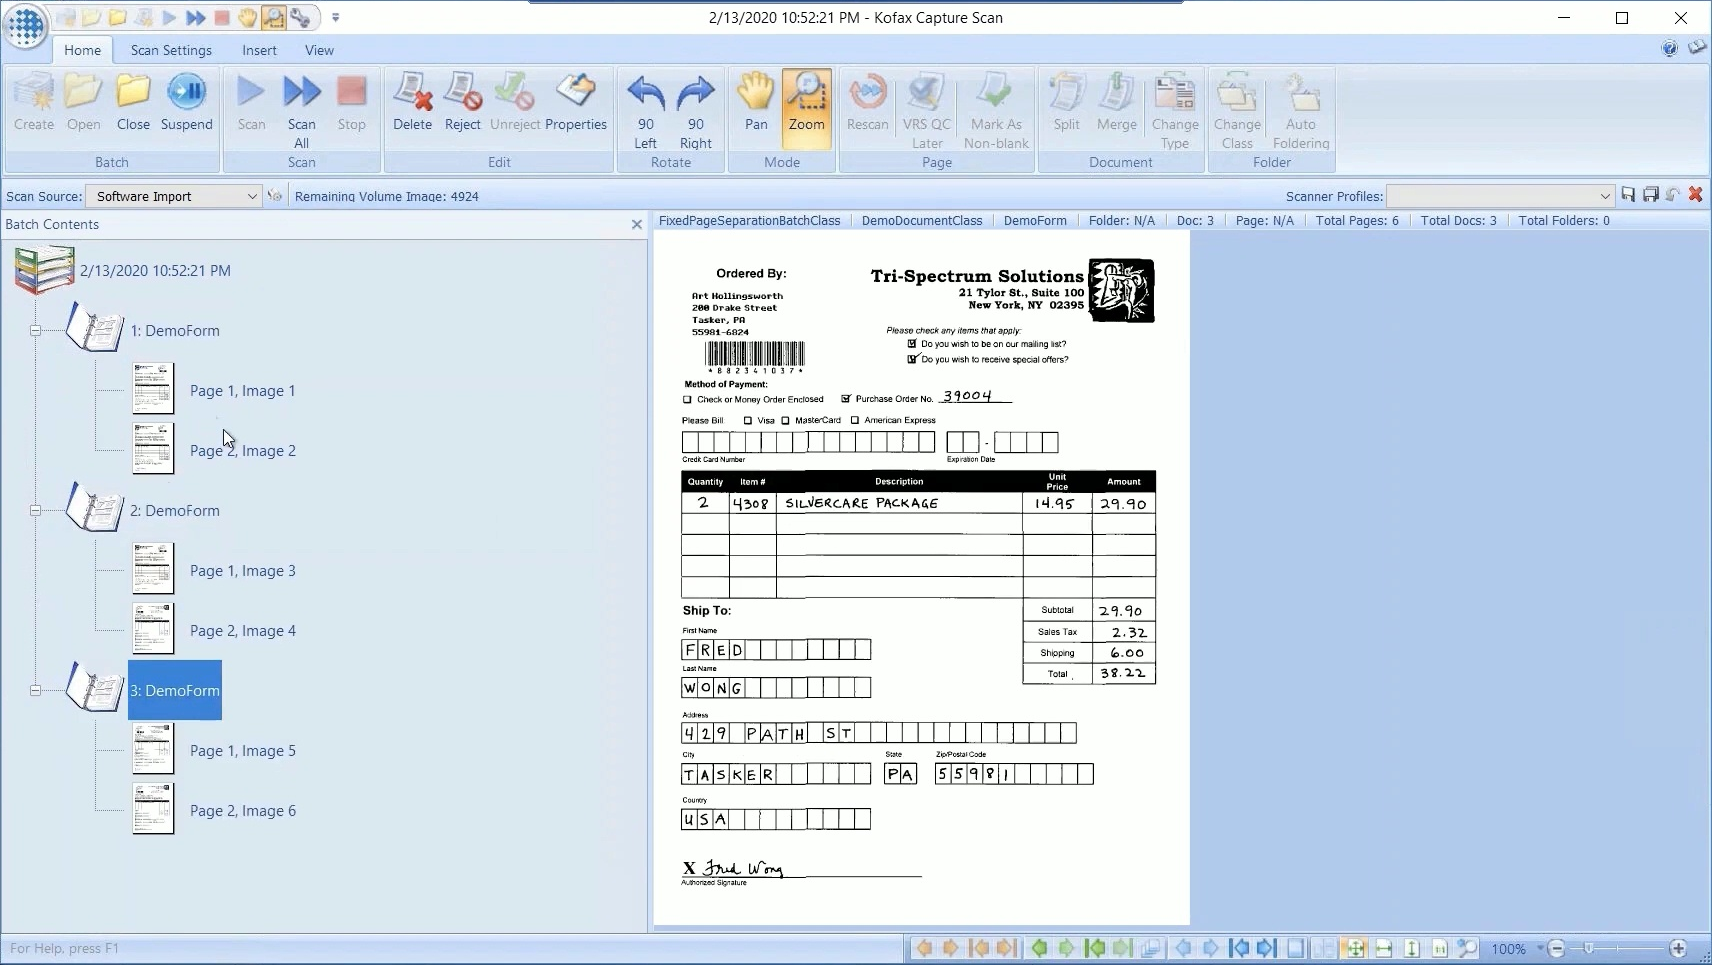
\includegraphics[width=\textwidth]{imaxes/b-estado-arte/kofax-capture}
        \label{fig:hough-punto-imagen}
    \end{subfigure}
    \begin{subfigure}[b]{0.9\textwidth}
        \centering
        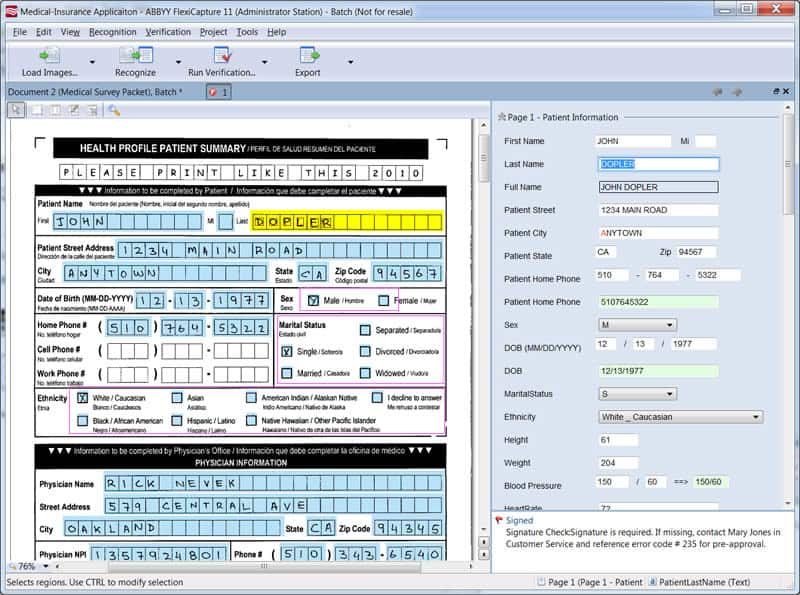
\includegraphics[width=\textwidth]{imaxes/b-estado-arte/abbyy-flexicapture}
        \label{fig:hough-intersection}
    \end{subfigure}
    \caption{Kofax Capture (arriba) y ABBYY FlexiCapture (abajo)}
    \label{fig:kofax-capture-y-abbyy-flexicapture}
\end{figure}

\subsection{Grooper}

Grooper \cite{solucionesComerciales_bisok_grooper} (ver imagen \ref{fig:grooper-bisok}) está hecho por Bisok y a priori parece seguir próxima en características a las dos anteriores. No obstante durante la búsqueda de información ha llamado la atención la mala organización de la información en la web oficial donde no existe una página o documento lineal que explique las características de la aplicación. Una característica destacable es el uso de técnicas de Procesamiento de lenguajes naturales para encontrar párrafos y frases en un documento o ser capaz de distinguir las clausulas en un contrato. También permite seleccionar el engine de \emph{\acrlong{ocr}} utilizado entre un abanico de opciones.

\subsection{Capture de ChronoScan}

Capture de ChronoScan \cite{solucionesComerciales_chronoScanCapture_chronoScanDocumentCapture} (ver imagen \ref{fig:chronoscan-capture}) es una aplicación individual más limitada en funcionalidades que las anteriores. Soporta el flujo normal de lotes con documento pero no dispone de arquitectura cliente servidor por lo cual su uso puede ser más interesante para pequeñas empresas o usuarios individuales. En este sentido la licencia permite su uso sin restricciones siempre que no sea en un contexto profesional.

\subsection{DocAcquire}

DocAcquire \cite{solucionesComerciales_docAcquire_docAcquire} es una solución \emph{\acrlong{saas}} y no dispone de versión de escritorio. Se puede probar de forma gratuita acudiendo a la web oficial. Es la aplicación más simple de todas y, al menos en la versión de prueba, parece que las acciones están bastante limitadas. No se pueden eliminar tipos de documentos una vez creados. Utiliza en engine Tesseract para \acrshort{ocr}.

\subsection{Textract y Document AI}

Dos servicios diferentes a los productos anteriores pero aplicables al problema son, Textract de Amazon \cite{solucionesComerciales_amazon_textract} y Document AI de Google \cite{solucionesComerciales_google_documentAI}. Ninguno de los dos suporta el flujo de información explicado ni están pensados para ser solución para el usuario final. Lo que ofrecen es un \emph{\acrlong{api}} capaz de recibir documentos y generar información estructurada como salida. El caso de Textract es totalmente opaco y por tanto no configurable. La salida consiste en ficheros JSON donde puede haber varios tipos de objetos: páginas, líneas y palabras, información de formularios (pares clave-valor), tablas, y elementos seleccionables como casillas. Además es capaz de identificar notas manuscritas. El servicio de Google permite definir \emph{processors}, que son plantillas específicas para modelos de documentos concretos. Actualmente parece que el servicio es muy reciente y está mayormente en beta. Cualquiera de ellos podría utilizarse para construir una solución más completa. Como otros servicios en la nube, el coste depende de la carga de trabajo procesada.

Después de revisar todas estas alternativas uno de los elementos comunes es el procesado por lotes. En general se deja en manos de los usuarios definir cómo son los modelos de los documentos por medio de un editor que selecciona regiones fijas y les asigna una topología. Estas dos características apuntan a que el sistema.

\begin{figure}
    \centering
    \begin{subfigure}[b]{0.9\textwidth}
        \centering
        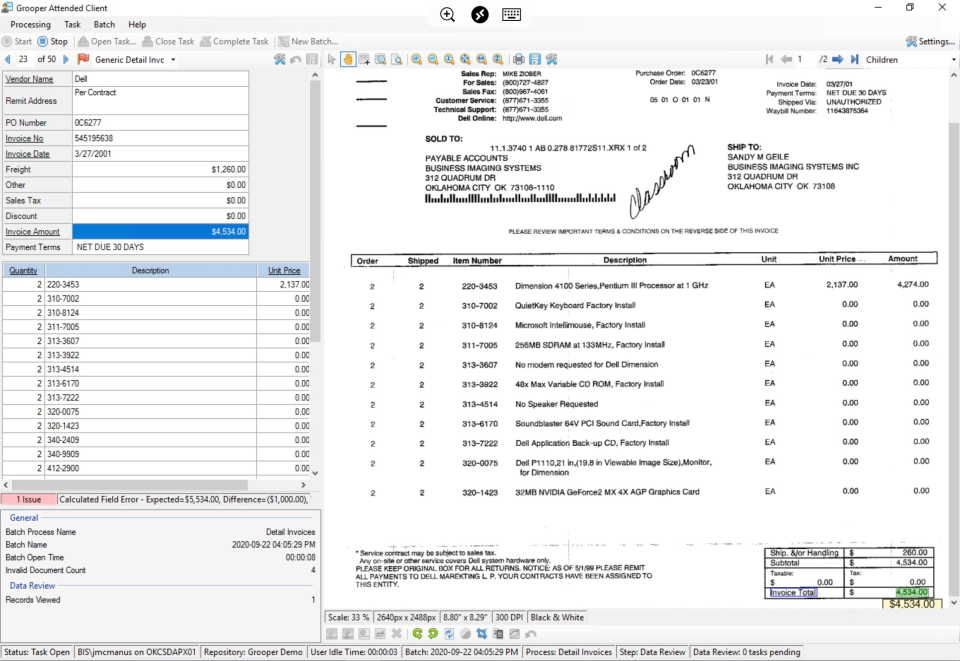
\includegraphics[width=\textwidth]{imaxes/b-estado-arte/bisok-grooper}
        \caption{Grooper, la solución de Bisok}
        \label{fig:grooper-bisok}
    \end{subfigure}
    \begin{subfigure}[b]{0.8\textwidth}
        \centering
        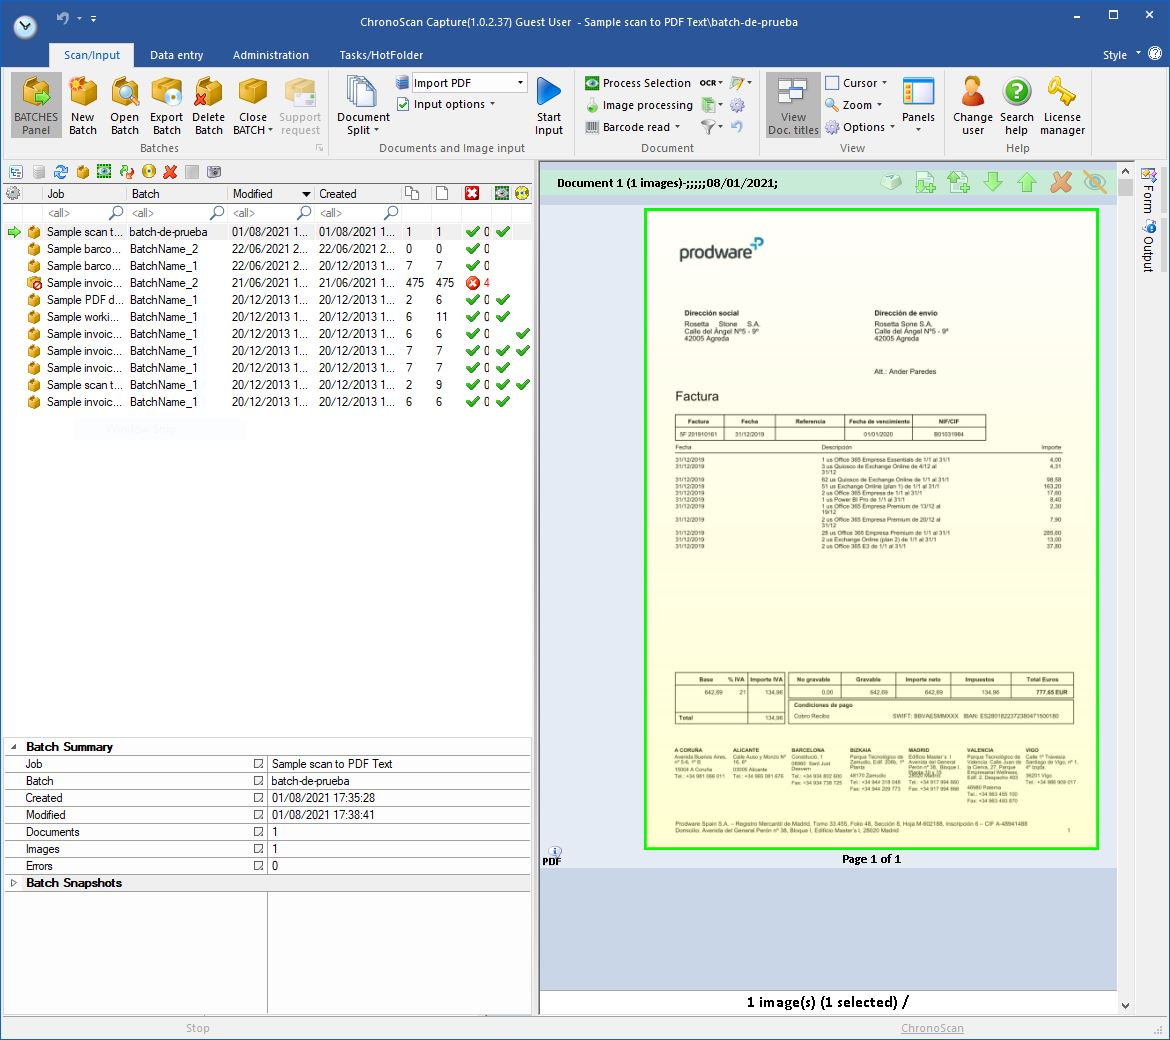
\includegraphics[width=\textwidth]{imaxes/b-estado-arte/chronoscan-capture}
        \caption{ChronoscanCapture con uno de los documentos usando en el proyecto}
        \label{fig:chronoscan-capture}
    \end{subfigure}
%    \caption{Kofax Capture (arriba) y ABBYY FlexiCapture (abajo)}
%    \label{fig:grooper-y-chronoscan-capture}
\end{figure}
 %%%%                %%%%
%%%% BASES TEÓRICAS %%%%
%%%%                %%%%

\chapter{Bases teóricas}
\label{chap:bases-teoricas}

\lettrine{E}{l} objetivo de este capítulo es sentar las bases tecnológicas y teóricas sobre las que se ha llevado a cabo el proyecto. En particular, se expone de qué manera se consiguen las coordenadas de las palabras y qué tecnologías intervienen para la obtención de la salida en formato estructurado.

Las aplicaciones comerciales utilizan las ubicaciones para seleccionar contenidos relevantes. Lo habitual es que el usuario pueda marque rectángulos sobre las páginas y los procesos de extracción y verificación únicamente tengan en cuenta estas áreas. Para poder hacer esto se necesitan las localizaciones de las palabras, pares clave-valor, tablas, etc. Entre los PDF manejados para la elaboración de este trabajo hay dos categorías importantes: aquellos que tienen texto directamente extraíble y otros donde cada página es una imagen. El primer caso es el habitual en los PDF generados con procesadores de textos u otros software. Se puede comprobar fácilmente si un PDF contiene texto directamente extraíble abriendo el documento con un visor y realizando la selección con el ratón. Si es el caso, se puede evitar hacer OCR del documento y obtener una versión sin errores del texto.

\section{Software para la manipulación de PDF}

Existen librerías y también aplicaciones capaces de manipular ficheros PDF para extraer texto, imágenes, reordenar páginas y otras muchas posibilidades. Para los objetivos del proyecto, sería necesaria una herramienta capaz de extraer el texto pero también sus coordenadas sobre el documento. Se revisaron varias alternativas, como PDFBox 
\footnote{https://pdfbox.apache.org/}, Win2PDF 
\footnote{https://www.win2pdf.com/doc/command-line-extract-text-pdf.html}, ebook-convert 
\footnote{https://manual.calibre-ebook.com/es/generated/es/ebook-convert.html}, que forma parte de la aplicación Calibre, y pdftotext 
\footnote{https://poppler.freedesktop.org/}. Únicamente esta última ofrece la posibilidad de generar las localizaciones necesarias.

La implementación original de esta utilidad fue realizada por Glyph \& Cog, autores del visor Xpdf. En el año 2005 surge la librería Poppler a partir del fork de la versión 3.0.3 de Xpdf. Esta es la implementación disponible mayormente en las distribuciones Linux. Por ejemplo, en Ubuntu se puede instalar con el paquete \verb|poppler-utils| e incluye otras muchas herramientas relacionadas.

Cuando se invoca la herramienta con el parámetro \verb|-bbox| se genera una salida en lenguaje XHTML. Esta variante del HTML tiene la ventaja de ser admitida por cualquier parser XML. Se identifican tags para los elementos que representan bloques, lineas y palabras. En cada uno se informa con cuatro valores de la localización del rectángulo que engloba al elemento: \emph{xMin}, \emph{xMax}, \emph{yMin}, \emph{yMax}. La generación de información de coordenadas o bounding box, además del texto, existe gracias a una aportación al proyecto del año 2010 de Kenneth Berland. 

\begin{figure}[hp!]
    \centering
    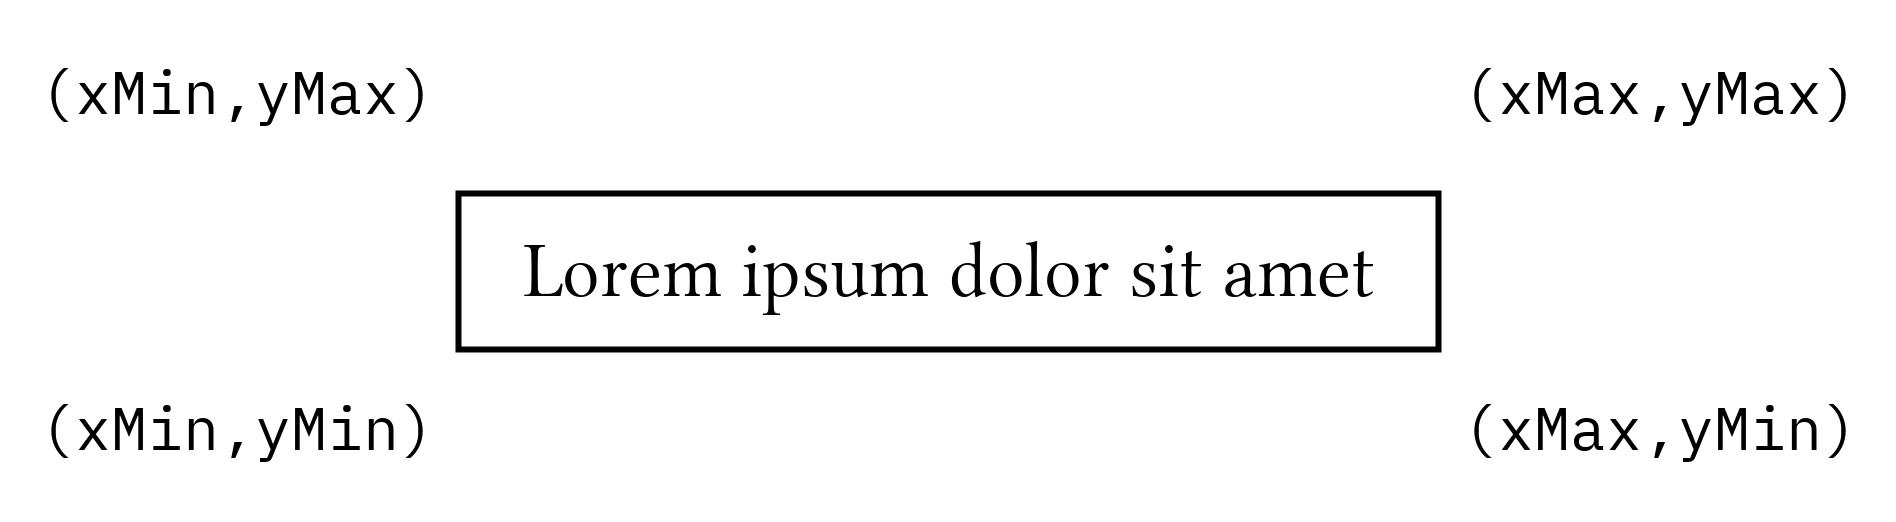
\includegraphics[width=0.75\textwidth]{imaxes/c-bases-teoricas/correspondencia-coordenadas-bounding.png}
    \caption{Correspondencia de las coordenadas en una bounding box}
    \label{fig:bounding-box}
\end{figure}

Una limitación común en todas estas utilidades consiste en no respetar el layout del texto, tal como aparece en el documento original. Esto implica que algunos elementos pueden aparecer antes que otros en la información extraída. Otro problema es que hay palabras que aparecen con caracteres intermedios, espacios, por ejemplo, que no se ven en el PDF. Estas limitaciones se derivan del propio funcionamiento del formato PDF.

\section{El formato PDF}

PDF es un formato digital para la creación de documentos. Fue introducido por Adobe Systems en 1993. En los siguientes años, el uso de este formato se extendió por toda la sociedad, tanto en el ámbito público como en el privado. En el año 2008, la ISO publicó el estándar 32000-1, tomando como base especificación de PDF en su versión 1.7, creada y liberada por Adobe. Posteriormente se publicó la versión 2.0 como ISO 32000-2 en el año 2017 y más recientemente una actualización en el año 2020. PDF es un modelo de representación de imágenes que deriva del lenguaje PostScript, también desarrollado por Adobe. En PDF, el modelo de imagen admite gráficos y texto de forma independiente al dispositivo de salida.

% TODO Considerar si añadir más información de PostScript.

\subsection{Almacenamiento de información}

Un PDF no es un fichero de texto, es un fichero binario de 8 bits con una estructura interna determinada. Sus elementos básicos son los objetos. Cualquier información que se visualice en el documento existirá realmente como un objeto dentro del fichero. Estos objetos están serializados dentro del fichero y pueden ser de alguno de los siguientes nueve tipos:

\begin{enumerate}
    \item \textbf{Null}: se utiliza para indicar la ausencia de un valor.
    \item \textbf{Boolean}: indica los valores de verdad true o false.
    \item \textbf{Integer}: representa valores enteros. Puede aparecer como \verb|1|, \verb|+2|, \verb|-100|.
    \item \textbf{Real}: representa valores decimales y puede aparecer como \verb|0,05|, \verb|.25|, \verb|-3,1415|.
    \item \textbf{Name}: son secuencias únicas dentro del fichero, comienzan con una barra. Por ejemplo: \verb|/Type|, \verb|/ThisIsName|.
    \item \textbf{String}: puede ser de 4 tipos:
    \begin{itemize}
        \item ASCII: bytes codificados en ASCII.
        \item PDFDocEncoded: bytes codificados con la codificación PDFDocEncoding.
        \item Text: bytes codificados en PDFDocEncoding o UTF-16BE.
        \item Date: utilizado para fechas. Se codifican en ASCII con un patrón de fecha. \footnote{D:YYYYMMDDHHmmSSOHH’mm}.
    \end{itemize}
    \item \textbf{Array}: es una colección heterogénea de objetos. Se escriben entre corchetes: \verb|[ 0 20 (E) ]|.
    \item \textbf{Dictionary}: es una tabla asociativa que contiene pares clave/valor. Pueden contener valores anidados y es utilizado para crear la jerarquía de todos los objetos del documento. Para indicar el comienzo y fin se utilizan los símbolos \verb|<<| y \verb|>>|. Las claves se indican con valores de tipo name.
    \item \textbf{Streams}: son secuencias de bytes de 8 bits sin límite de tamaño. Son utilizados para almacenar cualquier información binaria, por ejemplo imágenes, ficheros JSON o tipografías. Los stream tienen como preámbulo un diccionario de propiedades del stream. Este diccionario siempre debe contener, al menos, la clave \verb|/Length| que indica en bytes el tamaño del stream. Otra clave importante es \verb|/Filter|. \verb|/Filter| indica que la información está comprimida o codificada. Las imágenes se suelen codificar como DCTDecode o JPXDe que son versiones diferentes del formato JPEG. Para otro tipo de datos está disponible el algoritmo FlateDecode, similar a  DEFLATE, el mismo utilizado en los ficheros ZIP.
\end{enumerate}

Los objetos presentados hasta el momento son los objetos directos. Los objetos directos tienen el valor almacenado en el propio objeto. También existen los objetos indirectos que se referencian indirectamente y el consumidor tiene que saltar a otra posición en el fichero. Los objetos indirectos tienen un identificador único dentro del fichero. Las referencias son de la forma: \verb|/ObjIndirecto  5 0 R|.

\subsection{Estructura en un fichero}

La estructura de un fichero está dividida en cuatro partes, tal como se muestra en la figura \ref{fig:secciones-pdf}: header, body, cross-reference table y trailer. El header tiene al menos dos líneas. La primera se utiliza para indicar que el fichero es un PDF y la versión del estándar que le corresponde. La segunda es simplemente un separador: \verb|%%EOF|. 

\begin{figure}[hp!]
    \centering
    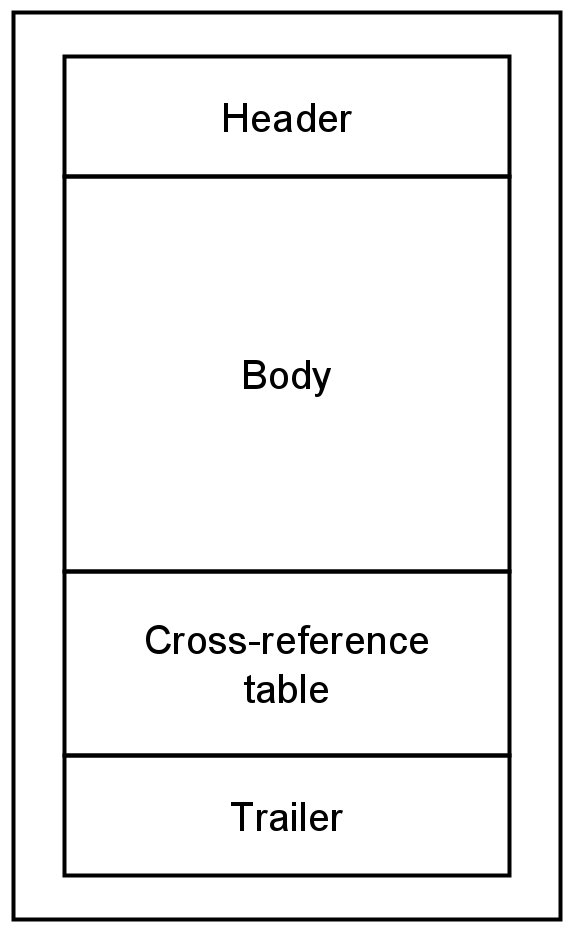
\includegraphics[width=0.3\textwidth]{imaxes/c-bases-teoricas/secciones-de-un-pdf.png}
    \caption{Las cuatro secciones de un PDF}
    \label{fig:secciones-pdf}
\end{figure}

El trailer es un objeto de tipo diccionario. Contiene claves y valores que aportan información a nivel de documento. Hay dos claves especialmente importantes, /Size que indica el número de entradas de la Cross-reference table y /Root que apunta al objeto que contiene el comienzo del Catálogo. El body contiene el objeto del Catálogo y todos los demás objetos que conforman el contenido del fichero PDF. La Cross-Reference Table es un índice de todos los objetos indirectos del PDF. Se utiliza para implementar la navegación sobre el fichero. Contiene la información necesaria para poder realizar saltos a la posición donde se encuentra el objeto que se quiere leer. La versión tradicional tiene tres columnas y la secuencia de entradas hace referencia al número del objeto buscado. En el ejemplo, para encontrar el objeto 2, tercera entrada, hay que saltar hasta el byte 32800:

\begin{lstlisting}[caption={Entradas en la Cross-Reference Table},label=lst:cross-ref-table]
0000000000 65535 f
0000000009 00000 n
0000032800 00000 n
0000000203 00000 n
0000000298 00000 n
0000008654 00000 n
0000000335 00000 n
\end{lstlisting}

% TODO Considerar hablar del catálogo o dejarlo para la parte de implementación.

%%%%%

\section{Representación de coordenadas en orígenes OCR}

La representación de las localizaciones de los elementos identificados por el proceso OCR es solo una parte de toda la información que se genera como salida de un engine. Existen varias propuestas de formatos que se proponen como formatos abiertos con intención de favorecer su adopción. Es el caso de hOCR \cite{ocrRepres_hocr_breuel_spec}, ALTO \cite{ocrRepres_alto_spec}, PAGE \cite{ocrRepres_page_pletschacher_paper} y TEI \cite{ocrRepres_tei_project}. Los tres últimos emplean XML como base y definen las etiquetas necesarias. La transformación entre ellos es posible y existe al menos un proyecto capaz de hacerlo
\cite{ocrRepres_conversion_ocrFileformat}. hOCR es el formato de representación escogido para el proyecto, como se verá en \ref{sec:rec-optico-caracteres}.

\subsection{El microformato hOCR}

hOCR es un estándar abierto que utiliza HTML como base tecnológica. Se diseñó siguiendo el modelos de los microformatos. Los microformatos son una tecnología ligada al auge de los blogs durante el año 2004. Su objetivo es aportar significado semántico a construcciones HTML, que de otro modo no lo tendrían ya que no forman parte como tal del lenguaje. La especificación hOCR hace uso de etiquetas \verb|DIV| y \verb|SPAN| para los elementos. Para la información se utilizan atributos como \verb|class|, \verb|title| o \verb|style|. Se combina con CSS para ampliar las capacidades del HTML en cuanto a representación de la salida OCR. HTML tiene soporte nativo para muchas características habituales en los documentos como estilo, tipografías, espaciado, etc.

La especificación hOCR define tres tipos de marcado:

\begin{itemize}
    \item Un marcado a \textbf{nivel lógico} que permite definir las secciones de un documento como en una estructura de tipo árbol.
    \item Un segundo tipo de marcado para representar el \textbf{nivel tipográfico y de división entre páginas}. Tiene la capacidad de modelar el documento de forma  que sus elementos principales se trasladarían al formato impreso de forma correcta. Este modelo se apoya en los procesos habituales que consideran el documento como un conjunto de bloques y elementos que se deben trasladar a su posición correcta.
    \item Un ultimo tipo para el \textbf{nivel físico} representado por líneas, figuras, y las palabras. Es específico para la implementación de cada motor de OCR. 
\end{itemize}

El formato proporciona también información geométrica, posiciones, de las palabras y valores de confianza respecto a la calidad que el motor valora sobre el reconocimiento realizado.

\section{Reconocimiento Óptico de Caracteres}
\label{sec:rec-optico-caracteres}

Para realizar el Reconocimiento Óptico de Caracteres se seleccionó Tesseract \cite{ocr_tesseract_raysmithetal.TesseractocrTesseract2021}. Existen otros de fuente abierta que se pueden considerar:

\begin{itemize}
    \item \textbf{OCRopus} \cite{ocr_ocropus_ocropy_project}, \textbf{Kraken}  y \textbf{Calamary} \cite{ocr_calamari_journal}: OCRopus es una colección de herramientas más que un producto final. Kraken y Calamary son forks de OCRopus que proporcionan un producto final. Sin embargo los tres proyectos están enfocados en resolver el problema de reconocer textos históricos con tipografías clásicas. Revisando la documentación de los tres no se encontró modelos preentrenados en castellano.
    \item \textbf{EasyOCR} (\cite{ocr_easyocr_official}, \cite{ocr_easyocr_project}) es la alternativa más viable. Es un proyecto que se actualiza regularmente y tiene soporte comercial. Como punto negativo destaca que aunque proporciona información de bounding-box, no sigue ninguno de los estándares comentados con anterioridad.
\end{itemize}

\textbf{Tesseract} \cite{ocr_tesseract_smith_paper} es un engine de código abierto y desarrollado inicialmente por Hewlett Packard \cite{ocr_tesseract_v4_release_notes} entre los años 1985 y 1995. Después de un periodo sin actividad, en el 2006 el proyecto fue recuperado por Google, que lo mantiene desde entonces. Hoy en día tiene soporte para más de cien idiomas y la red neuronal que emplea \footnote{Desde la versión 4, Tesseract utiliza una red LSTM. Esta es una red neuronal de tipo recurrente o RNN.} puede ser entrenada para casos específicos, si se necesita. Existe una amplia documentación en la web oficial, además, numerosos tutoriales en la red permiten familiarizarse con la herramienta. Es un proyecto bien conocido y de larga trayectoria.

\section{Detección de líneas tablas}

Los documentos contienen tablas donde hay dibujadas rectas que separan dos líneas de contenido. La Transformada de Hough (\cite{hough_krishna_computerVision}, \cite{hough_grauman_presentation}) proporciona una manera automática de delimitar esos espacios.

Este algoritmo es una técnica de visión por computador utilizada para detectar figuras tales como líneas o círculos. Se puede aplicar a cualquier figura siempre que se conozca una ecuación paramétrica que la defina. A continuación se detalla el funcionamiento general del algoritmo.

Se utiliza como entrada la información obtenida al aplicar un detector de bordes en la imagen original. Si se considera un punto borde cualquiera, sobre él pueden pasar infinitas rectas. Estas rectas se pueden definir con la ecuación \ref{hough-ecu-recta}.

\begin{equation}
    \label{hough-ecu-recta}
    y = a*x + b
\end{equation}

Reescribiendo la ecuación como,

\begin{equation}
b = -a*x + y
\end{equation}

es posible transformar cada punto borde al espacio de Hough y obtener una recta en dicho espacio.

Considerando dos puntos del espacio imagen \ref{fig:hough-punto-imagen}, al trasladarlos \ref{fig:hough-intersection} al es espacio Hough se puede calcular su intersección resolviendo el sistema de ecuaciones. Esta intersección proporciona los parámetros para construir, en el espacio imagen, la recta \ref{fig:hough-recta-a-b} que une ambos puntos.

\begin{figure}
    \centering
    \begin{subfigure}[b]{0.3\textwidth}
        \centering
        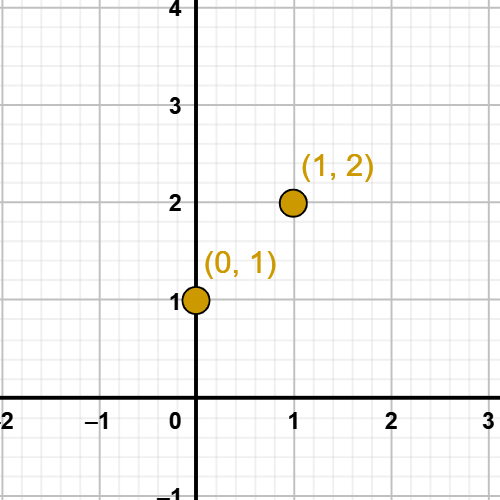
\includegraphics[width=\textwidth]{imaxes/c-bases-teoricas/hough-1}
        \caption{Dos puntos borde en el espacio imagen}
        \label{fig:hough-punto-imagen}
    \end{subfigure}
    \hfill
    \begin{subfigure}[b]{0.3\textwidth}
        \centering
        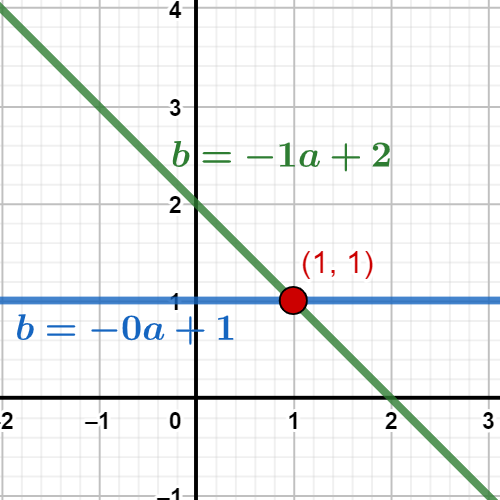
\includegraphics[width=\textwidth]{imaxes/c-bases-teoricas/hough-2}
        \caption{Rectas e intersección en el espacio Hough}
        \label{fig:hough-intersection}
    \end{subfigure}
    \hfill
    \begin{subfigure}[b]{0.3\textwidth}
        \centering
        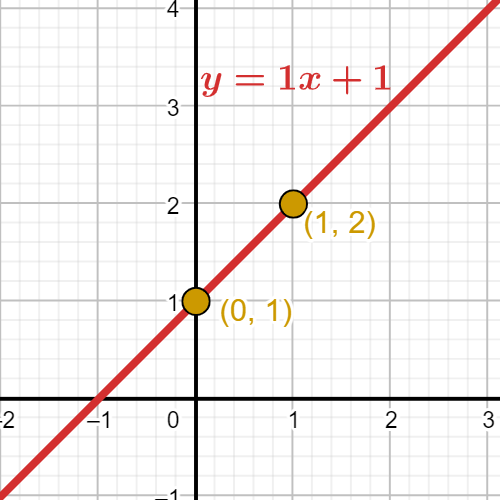
\includegraphics[width=\textwidth]{imaxes/c-bases-teoricas/hough-3}
        \caption{Recta que une ambos punto en el espacio imagen}
        \label{fig:hough-recta-a-b}
    \end{subfigure}
    \caption{Transformaciones del espacio imagen al espacio Hough}
    \label{fig:transformaciones-hough}
\end{figure}

El procedimiento general del algoritmo es como sigue:

\begin{enumerate}
    \item Se cuantiza el espacio de Hough. La cuantización divide el espacio en celdas.
    \item Se toma cada par de puntos de la imagen borde.
    \begin{enumerate}
        \item Se calcula su intersección.
        \item Se busca la celda donde coincide el punto intersección.
        \item Se aumenta en uno el recuento de votos de esta celda.
    \end{enumerate}
    \item Al final las celdas más votadas son las candidatas a ser líneas reales.
\end{enumerate}

\section{Análisis léxico y sintáctico}

\subsection{Introducción}

Como parte del proyecto se han desarrollado una herramienta que utiliza análisis léxico/sintáctico para generar una salida estructurada. Estos analizadores son una parte de los pasos que habitualmente realiza un compilador para obtener un programa ejecutable.

\subsection{Conceptos básicos}

\begin{itemize}
    \item Un \textbf{lenguaje} es un conjunto de cadenas de longitud finita creadas a partir de un alfabeto finito.
    \item Un \textbf{token} es la unidad mínima que se caracteriza por aportar significado léxico. En un lenguaje de programación cualquier palabra reservada es un token.
    \item Un \textbf{árbol de derivación} es
    \item El \textbf{axioma} en una gramática es el elemento desde el que se construyen todos los árboles de derivación en la gramática
    \item Las \textbf{producciones} son reglas de sustitución para la generación de cadenas del lenguaje.
\end{itemize}

\subsection{Lenguajes formales}

La teoría de autómatas y lenguajes formales es uno de los pilares que definen el funcionamiento de los ordenadores. Con esta teoría se pueden construir los compiladores utilizados en los lenguajes de programación.

En los años 30 del siglo XX Alan Turing ideó el modelo de una máquina abstracta que posee las mismas capacidades de cálculo que los ordenadores actuales. 

Posteriormente en los años 50, Noam Chonsky durante el estudio de la construcción de lenguajes naturales comienza el estudio de las gramáticas formales.

En primer lugar hay que entender qué es un lenguaje. Tomando una colección finita de símbolos se puede construir secuencias con ellos. Si se utilizan las letras del alfabeto, combinando los símbolos es posible construir cadenas que pertenecerán al castellano y también otras muchas que no pertenecen.

Una palabra es una secuencia determinada construida con símbolos que están en el alfabeto.

Un lenguaje es una conjunto de palabras o cadenas

Un autómata en su visión más inmediata es un diagrama que ayuda en encontrar las palabras de un lenguaje. Se utiliza un grafo dirigido con información adicional. Los nodos del grafo son los estados e indican en qué punto del análisis de la cadena se encuentra. Las aristas van etiquetadas con caracteres del alfabeto y se llaman transiciones

Un autómata especifica un lenguaje como el conjunto de aquellas cadenas que lo llevan del estado inicial a alguno de los estados de aceptación. Al mismo tiempo un autómata puede ser visto como un generador de las cadenas de un lenguaje si se comienza con la cadena vacía y se añaden símbolos según se recorren las transiciones, hasta llevar a un estado de aceptación.

A partir del diagrama de estados del autómata es posible obtener unas expresiones de la forma $A\rightarrow S$ que representan las mismas transiciones del autómata y pueden ser consideradas reglas de sustitución para la generación de cadenas.

Queda por tanto clara la relación existente entre las gramáticas, los lenguajes y los autómatas. Una gramática proporciona las reglas para identificar todas las construcciones que pertenecen a un lenguaje. El autómata es el modelo matemático abstracto capaz de recibir cadenas del lenguaje y decidir si son válidas para una gramática.

La notación Backus-Naur se utiliza para describir una gramática. Fue desarrollada por John Backus para el lenguaje Fortran y mejorada por Peter Naur para poder describir el lenguaje Algol 60.

La jerarquía de Chomsky define cuatro tipos de gramáticas dependiendo de la forma de las reglas de producción de la gramática.

\begin{figure}[hp!]
    \centering
    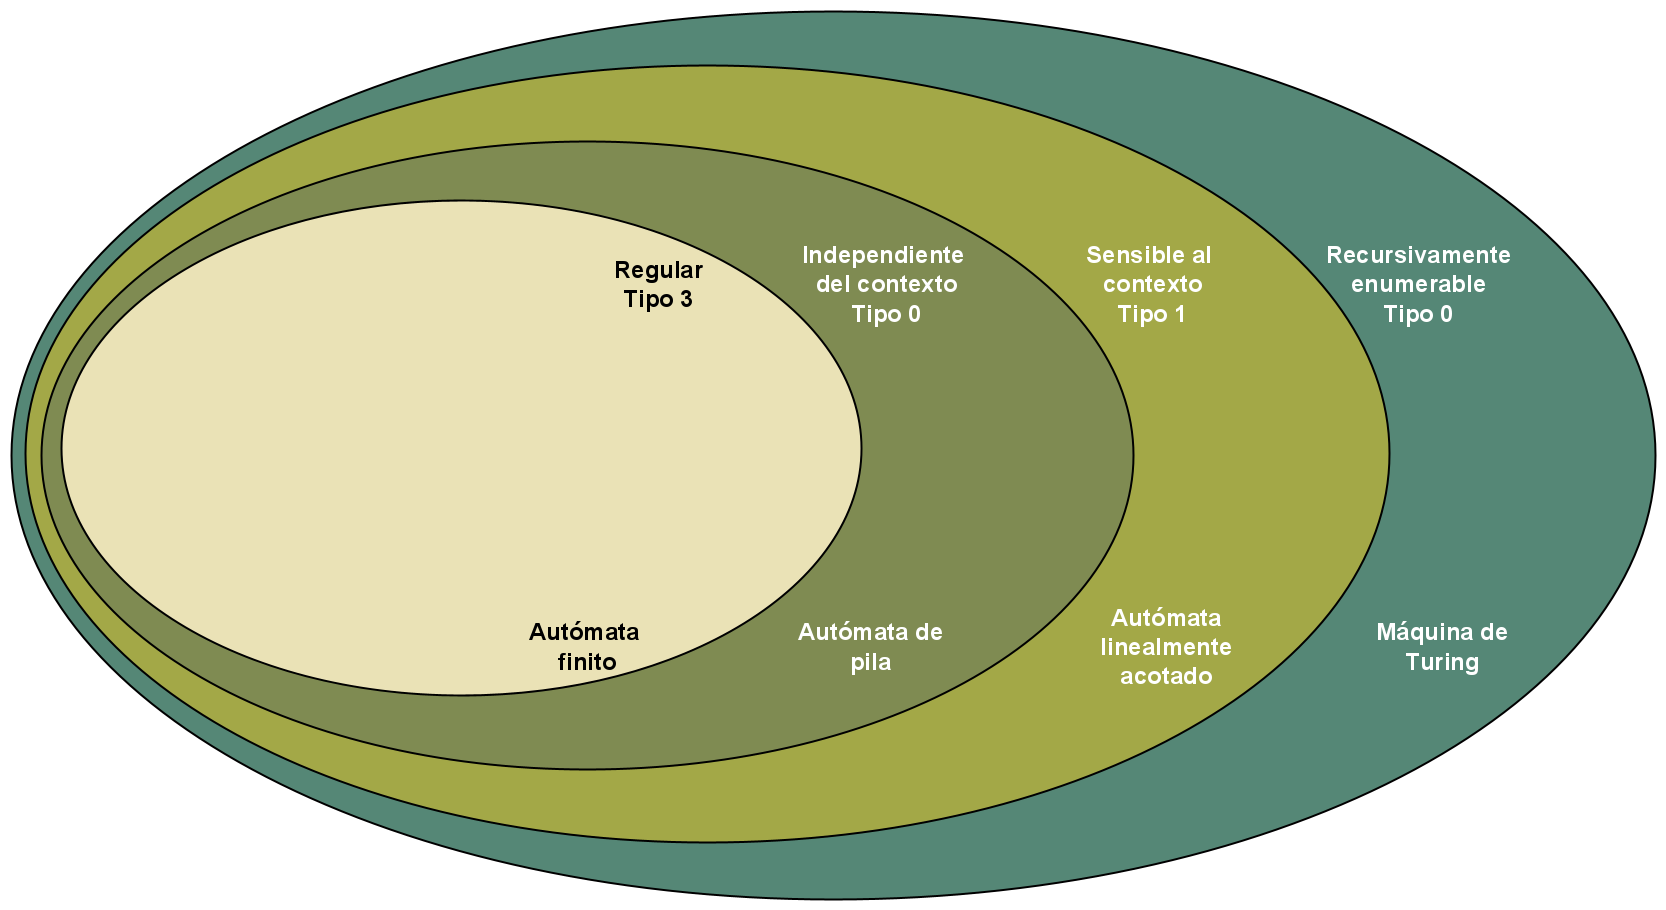
\includegraphics[width=1.0\textwidth]{imaxes/c-bases-teoricas/niveles-chomsky.png}
    \caption{Jerarquía de Chomsky}
    \label{fig:niveles-chomsky}
\end{figure}

\begin{enumerate}
    \item Gramáticas regulares
    \item Gramáticas independientes del contexto
   Una gramática independiente del contexto consta de cuatro componentes
   - Un conjunto de símbolos terminales, también llamados tokens
   - Un conjunto de no terminales que representa a un conjunto de cadenas o terminales
    - Un conjunto de producciones que tienen dos partes con una flecha que las separa. En el lado izquierdo siempre hay un no terminal. En el lado derecho hay un conjunto de terminales y no terminales
    - Uno de los no terminales es el símbolo inicial.
    El objetivo es aplicar sustituciones, para obtener las cadenas del lenguaje.
    
    \item Gramáticas dependientes o sensibles al contexto
    \item Gramáticas recursivamente enumerables
    \item Gramáticas recursivos (fuera de la jerarquía de Chomsky)
\end{enumerate}

\begin{figure}[hp!]
    \centering
    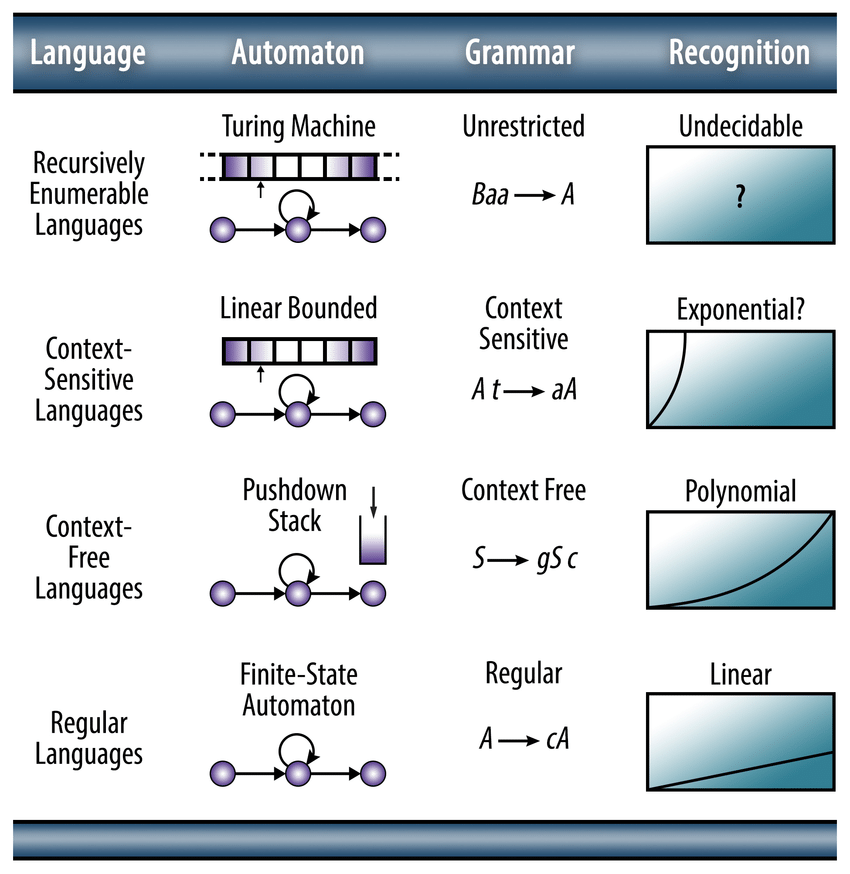
\includegraphics[width=0.6\textwidth]{imaxes/c-bases-teoricas/hauser-2016.png}
    \caption{Ejemplos de los 4 modelos con la dificultad de reconocimiento \cite{teoriaCompiladores_hauser_automatas}}
    \label{fig:hauser-2016}
\end{figure}

% TODO valorar si incluir los siguientes datos:

Algoritmos ascendentes LR
Algoritmos descendentes LL
LL Left Left: 1º entrada de izq a der, 2º se producen derivaciones por la izquierda
LR Left Right: 1º entrada de izq a der, 2º derivaciones por la derecha
Bison es LALR (lookahead LR)


\subsection{Fases de la compilación}

El proceso de compilación se divide en varias fases. En la imagen \ref{fig:analisis-lexico-sintáctico} se presenta un ejemplo del proceso completo que un compilador realiza para obtener la representación en código máquina desde el programa fuente. Las fases principales son las siguientes:

\begin{enumerate}
    \item El \textbf{análisis léxico} es el proceso por el cual se separa el texto de entrada, código fuente, en las unidades lógicas del lenguaje como identificadores, operadores o palabras clave. 
    Durante el análisis se comprueba la validez de los tokens identificados. Es habitual en los lenguajes de programación que la construcción de los identificadores siga unas reglas estrictas. El escáner utiliza expresiones regulares para comprobar la validez de los nombres.
    El analizador léxico y sintáctico comparten información de los identificadores por medio de la tabla de símbolos.
    La salida del analizador léxico es la secuencia de tokens reconocidos. Esta secuencia es la entrada del analizador sintáctico.
    
    \item En el \textbf{análisis sintáctico} se intenta encontrar un árbol sintáctico o árbol de derivación para una secuencia de tokens que tenga como raíz el axioma de la gramática. Si se encuentra, significa que la secuencia de tokens pertenece al lenguaje. En caso contrario el compilador notificará un error al usuario.
    
    Los analizadores utilizados en los compiladores suelen ser de tipo ascendente o descendente. En los ascendentes, el árbol se construye buscando un camino desde las hojas hasta el axioma. Con los descendentes pasa justo lo contrario. En cualquiera de los dos casos la entrada se trata de izquierda a derecha. 
    
    Los analizadores más habituales son de tipo LL (descendentes) o LR (ascendentes). La primera L indica que en ámbos casos la entrada se trata de izquierda a derecha. La segunda L en LL indica que la derivación se realiza por la izquierda. Y la R en LR indica que la derivación es por la derecha. En el caso de Bison, el analizador utilizado en el proyecto, es un parser de tipo LALR, lo que quiere decir es un LR que utiliza un símbolo de anticipación (\emph{look ahead} LR) para construir el árbol de derivación. 

    \item En la fase de \textbf{análisis semántico} se explota el árbol sintáctico y la tabla de símbolos con el propósito de verificar que el código fuente es consistente con el lenguaje. Algunos ejemplos de tareas realizadas en esta fase son la comprobación de los tipos que comprueba que las operaciones realizadas utilicen los tipos correctamente. Otro aspecto que se realiza es la conversión automática de ciertos tipos como sucede en el caso de Java con las operaciones de Autoboxing y Unboxing. El compilador en este paso añadiría la llamada al método correspondiente para para realizar la conversión entre tipos primitivos y objetos.
    
    \item La \textbf{generación de código intermedio} consiste en la creación de una representación no final del programa fuente. Tras el análisis léxico y sintáctico suele ser habitual generar una representación no final del programa fuente en un formato similar al código máquina pero pensado para una máquina abstracta en lugar de la máquina destino. Algunas tareas habituales en esta fase consisten en la reordenación de las sentencias en base a la prioridad de los operadores. También se produce la generación nombres temporales para los resultados de cálculos intermedios.
    
    \item La fase de \textbf{optimización del código} intermedio es utilizada para mejorar el código intermedio creando un mejor código para la máquina final. Estas mejoras afectarán a la complejidad del código, consiguiendo reducir el número de sentencias. Si el código tiene menos sentencias el programa final será más pequeño. También se traducir llamadas a métodos por valores finales, como en el caso de Autoboxing mencionado anteriormente. El número o cantidad de optimizaciones van a implicar unos tiempos de compilación muy diferentes. Los compiladores generales tratan de encontrar un equilibrio entre entre los dos parámetros. O se deja en manos del usuario especificar el nivel de optimización deseado.
    
    \item La generación del código final sirve para traducir la representación intermedia en el lenguaje de destino, como ensamblador para una máquina en particular. Primero se toma la representación y se asigna al lenguaje de destino. También se seleccionan los registros necesarios para las variables del programa. Luego las instrucciones en lenguaje intermedio se trasladan a las instrucciones de la máquina.

\end{enumerate}

\begin{figure}[hp!]
    \centering
    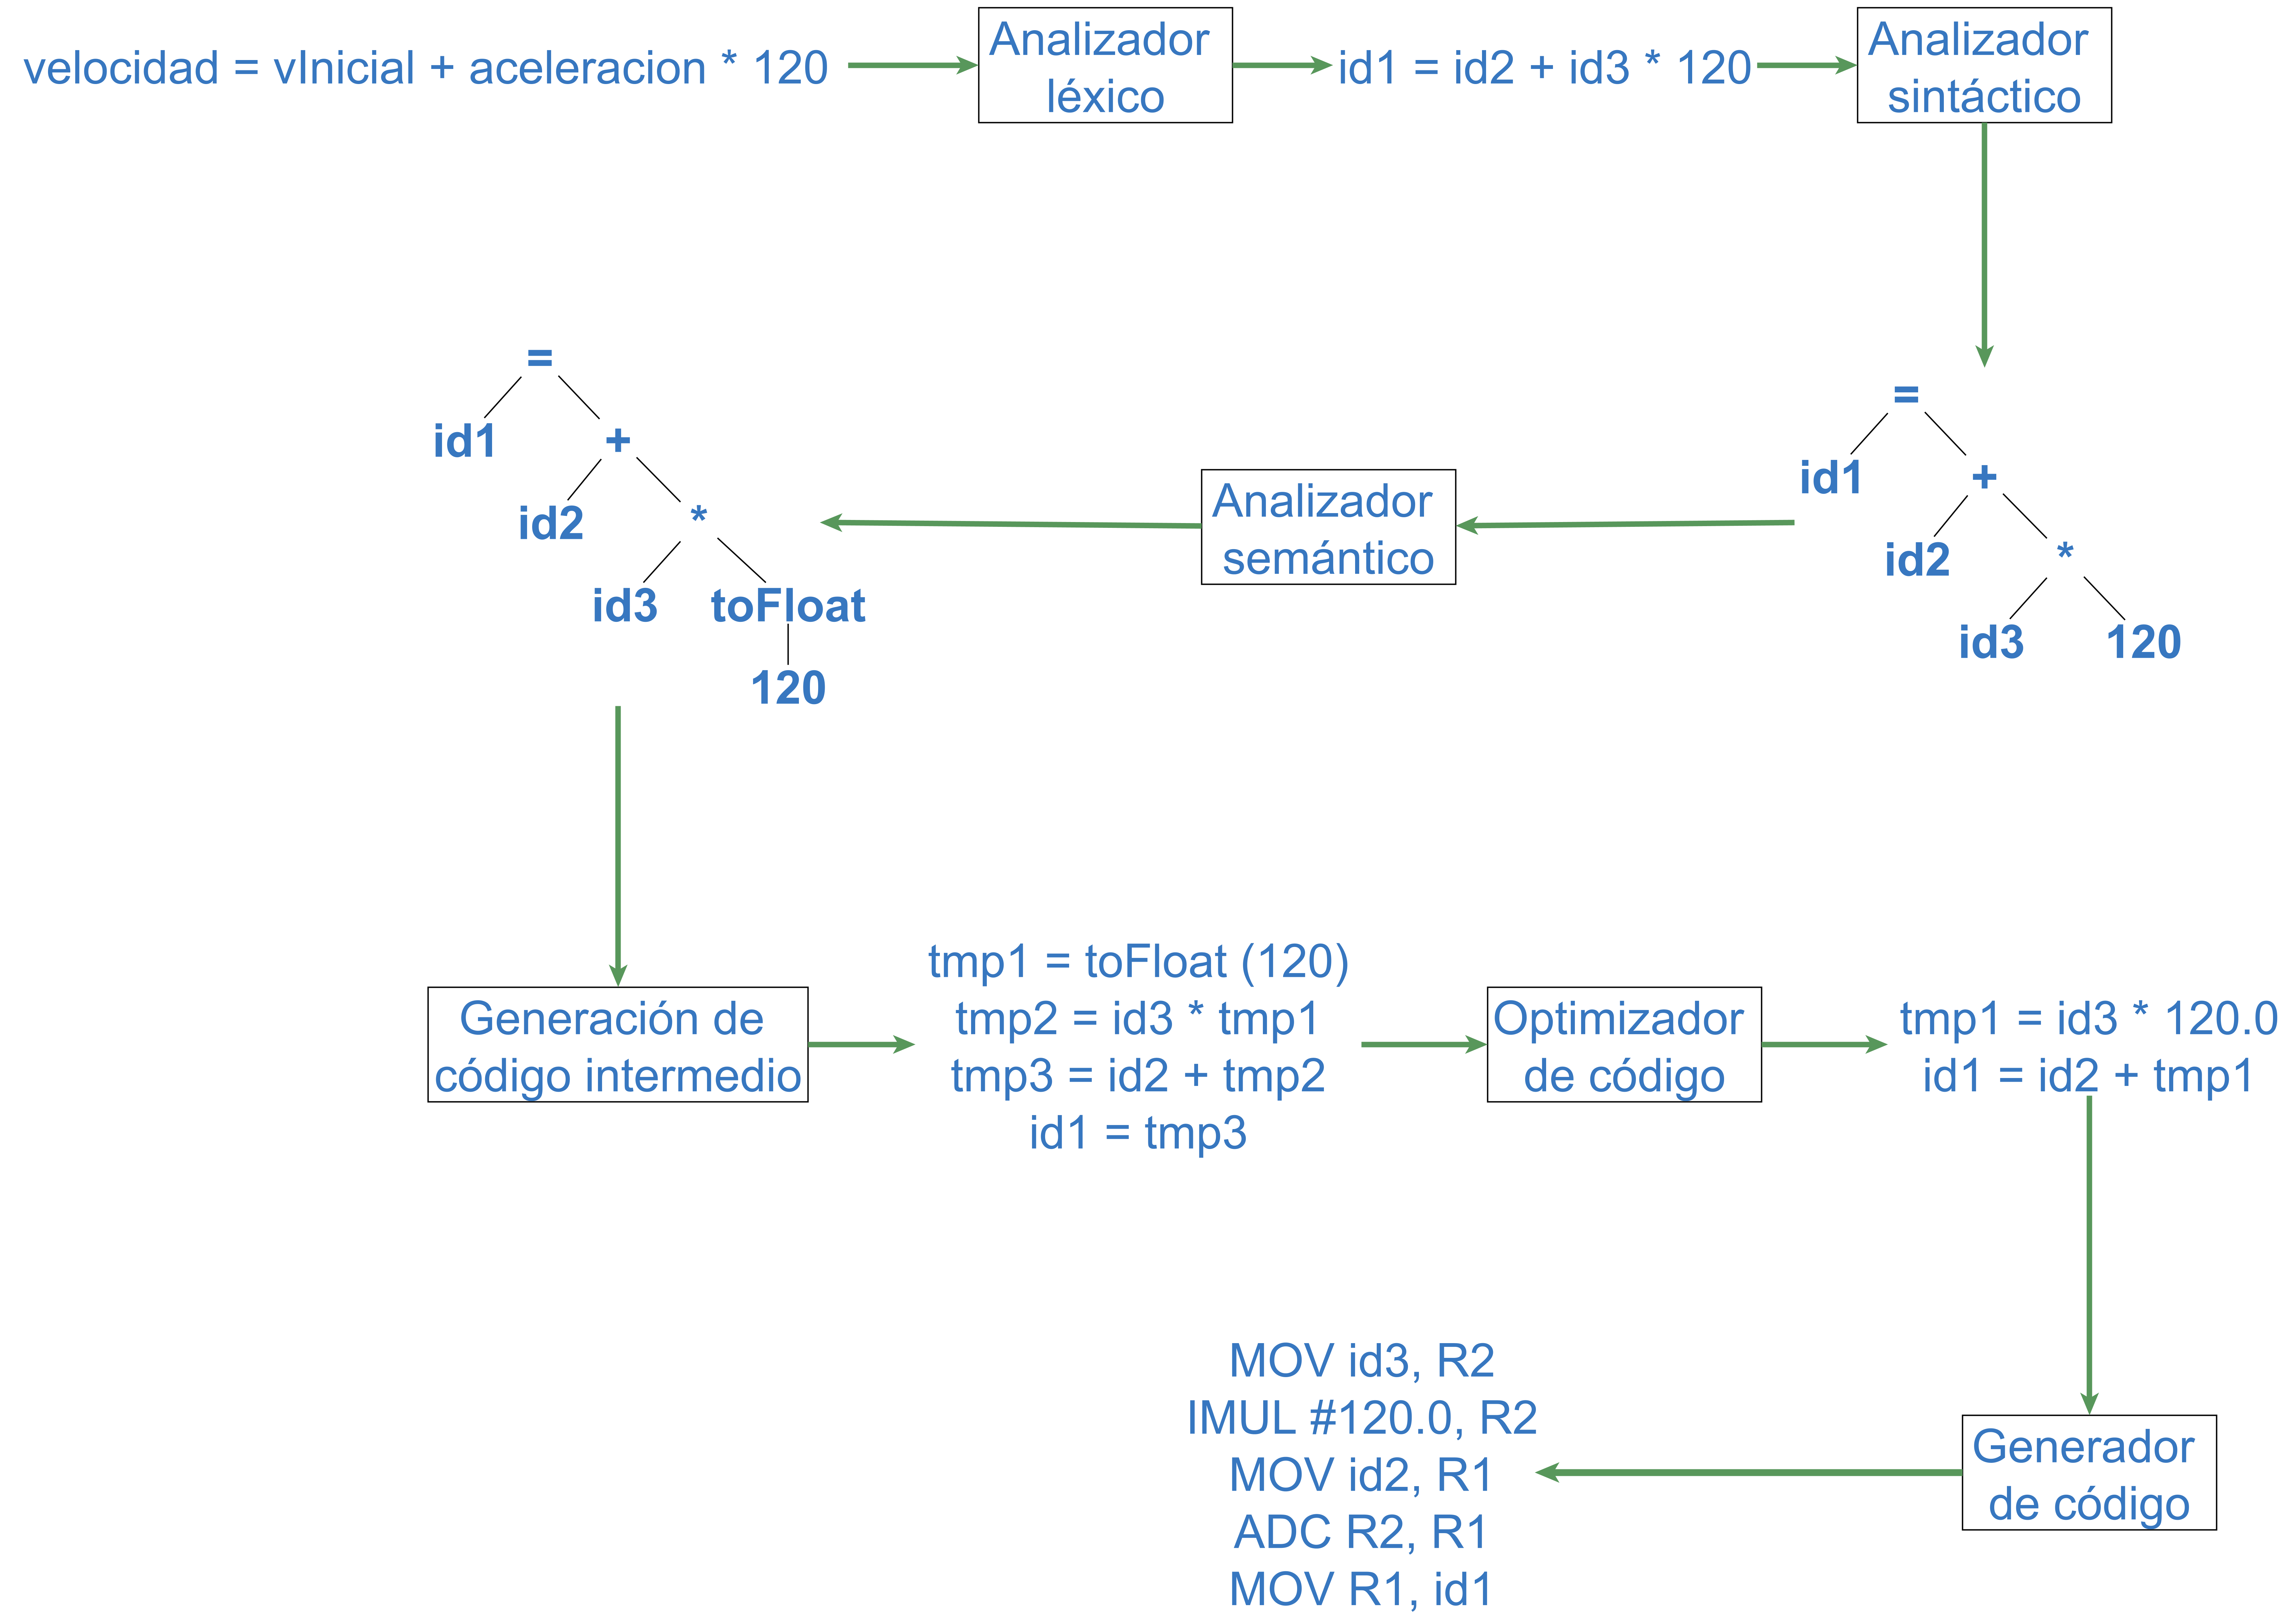
\includegraphics[width=1.0\textwidth]{imaxes/c-bases-teoricas/analisis-lexico-sintactico.png}
    \caption{Ejemplo del proceso de análisis de un compilador}
    \label{fig:analisis-lexico-sintáctico}
\end{figure}








 %%%%             %%%%
%%%% METODOLOGÍA %%%%
%%%%             %%%%

% TODO explicar cómo facilita Scrum la adaptación para la construcción del prototipo web

\chapter{Metodología}
\label{chap:metodologia}

\lettrine{E}{n} este capítulo trata sobre metodologías aplicadas a proyectos de software y en particular la metodología seleccionanda para el este trabajo, Scrum.

Las metodologías para que se refieren al Ciclo de Vida del Desarrollo de Software, SDLC en inglés, son procesos y prácticas utilizadas por los equipos de desarrollo de software para tratar con éxito el SDLC.

Históricamente la metodología más conocida es la metodología de desarrollo en Cascada que tiene su origen en un artículo científico de Winston W. Royce en los años 70. Esta metodología se completa en cinco etapas:

\begin{enumerate}
    \item Análisis de requisitos
    \item Diseño
    \item Implementación
    \item Verificación
    \item Mantenimiento
\end{enumerate}

Un proyecto se realiza en un único ciclo,  las etapas se ejecutan en orden y sin solapamientos. Este es un modelo que resulta rígido e impone muchas limitaciones: las pruebas de integración no se pueden llevar a cabo hasta completar todo el desarrollo, los usuario no puede probar la aplicación hasta el final del proyecto, que se puede demorar meses o incluso años. En este modelo no hay oportunidad para que los cliente u otras partes interesadas puedan ofrecer sus opiniones.

Para tratar de ofrecer una alternativa a las limitaciones impuestas por el desarrollo en cascada, fueron propuestas otras metodologías, como la metodología en espiral o la metodología en V. Pero no fue hasta mediados de los años 90 que no aparecen las primeras tecnologías ágiles. Especialmente en el año 2001 se publicó el Manifiesto por el desarrollo ágil que valora los siguientes cuatro puntos:

\begin{itemize}
    \item Individuos e interacciones sobre procesos y herramientas.
    \item Software funcionando sobre documentación extensiva.
    \item Colaboración con el cliente sobre negociación contractual.
    \item Respuesta ante el cambio sobre seguir un plan.
\end{itemize}

En este proyecto se utiliza Scrum que pertenece al conjunto de metodologías ágiles.

\section{Scrum}

\emph{The Scrum Guide} es la guía oficial donde se presenta el framework Scrum. Scrum es un marco de trabajo para ayudar en la creación de valor mediante soluciones adaptativas a problemas complejos. Scrum propone una filosofía general, varios roles para las tareas, unos eventos que se repiten de forma cíclica y unos artefactos como producto del trabajo.

Scrum no está limitado a proyectos de software. Siempre y cuando se respeten sus características, se posiciona como un modelo más general, que se puede aplicar a cualquier proyecto donde sea capaz de aportar valor.

\subsection{Roles}

La unidad de trabajo está formada por el Equipo Scrum. Se consideran tres roles dentro del Equipo:

\begin{itemize}
    \item Los \textbf{Desarrolladores} son todas las personas que contribuyen a crear los incrementos durante cada ciclo. Las cualidades de las personas consideradas desarrolladoras pueden ser variadas. Los desarrolladores son responsables del mantenimiento del Sprint Backlog.
    \item El \textbf{Product Owner} es la persona responsable de maximizar el valor resultante del trabajo del Equipo Scrum. El framework no indica como debe conseguir este objetivo. El Product Owner también es responsable del Product Backlog.
    \item El \textbf{Scrum Master} es responsable de asegurar que se siguen los principios del marco de trabajo y entre sus obligaciones está la de actuar apoyando a los demás miembros del equipo para la mejora de las prácticas relacionadas con Scrum. De forma general es responsable de la efectividad del Equipo.
\end{itemize}

\subsection{Eventos}

El ciclo de vida de Scrum está contenido en el Sprint. Durante un Sprint se lleva a cabo el trabajo generador de valor para el proyecto. La duración de un Sprint es flexible pero debería estar entre una y cuatro semanas. Debe ser lo suficientemente largo como para dar tiempo a la realización de trabajo significativo, pero no tan largo que se pierda de vista el objetivo del propio Sprint, o que el objetivo planificado cambie y ya no sea válido. Dentro del Sprint se suceden los otros cuatro tipos de eventos.

\begin{figure}[hp!]
    \centering
    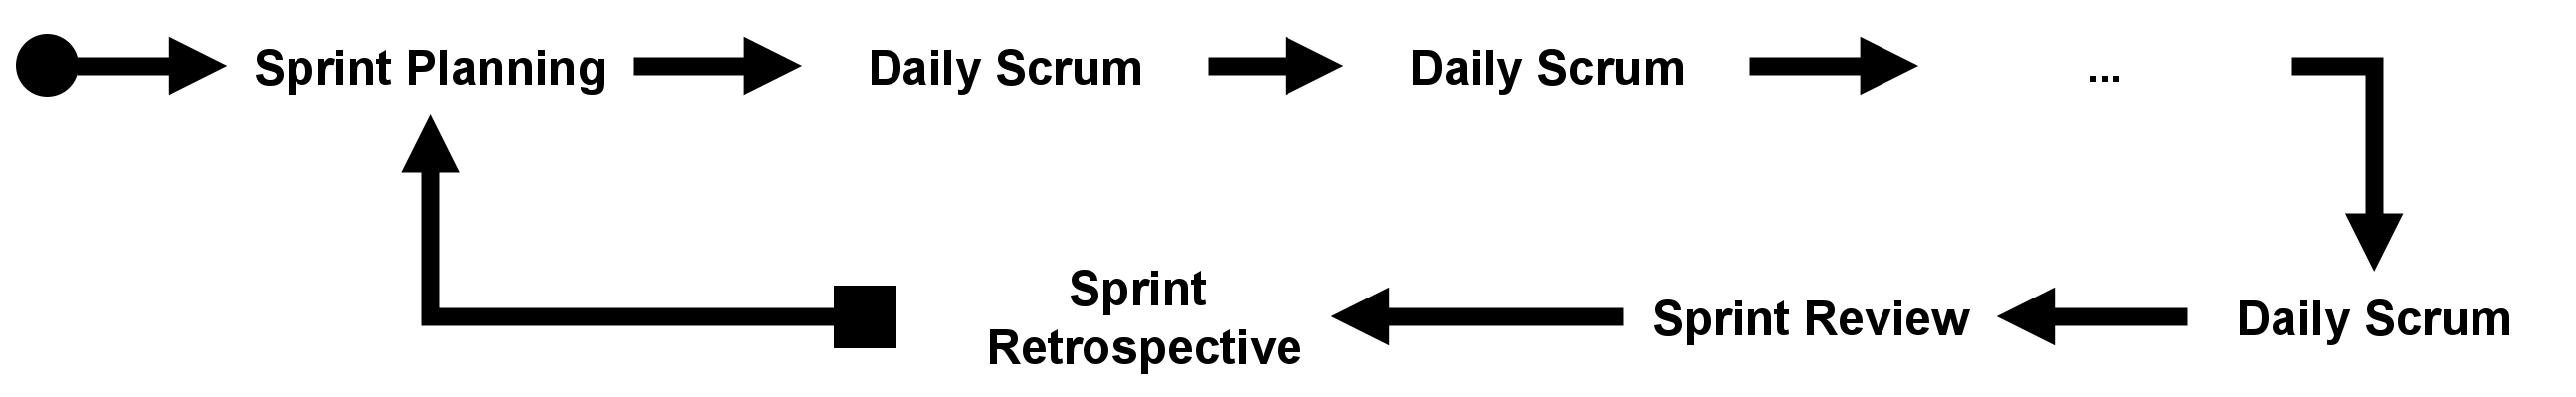
\includegraphics[width=1.0\textwidth]{imaxes/d-metodologia/ciclo-scrum.png}
    \caption{Ciclo de vida de Scrum.}
    \label{fig:ciclo-vida-scrum}
\end{figure}

\begin{itemize}
    \item El \textbf{Sprint Planning} es da comienzo a un nuevo Sprint. En este evento se acuerda el trabajo que se va a realizar durante el Sprint. El equipo completo trabaja para establecer las tareas particulares que serán abordadas en el periodo. En el Sprint Planning pueden participar otras personas involucradas con el proyecto pero que no pertenezcan al Equipo. Su ayuda puede ser necesaria para aclarar aspectos de las tareas o los objetivos.
    En este evento es importante dar respuesta a cómo se puede añadir más valor al producto. El Objetivo del Sprint debe quedar claramente definido y para ello todo el equipo colabora. También hay que establecer qué cosas se pueden llevar a cabo durante el Sprint. Se seleccionan por tanto todas aquellas tareas que deberán ser abordadas. Por último se requiere decidir cómo se llevarán a cabo las tareas. Puede ser necesario conseguir un mayor refinamiento para que los Desarrolladores puedan tomar las decisiones correspondientes.

    \item El \textbf{Daily Scrum} es un evento de 15 minutos para revisar el avance hacia el objetivo del Sprint. Como en otros aspectos de Scrum, el framework no explicita la técnica o estructura de la reunión, pero insiste en que es el momento de comunicar dificultades, logros y planificar el trabajo para la jornada siguiente. A esta reunión solo acuden los Desarrolladores.
    
    \item El \textbf{Sprint Review} tiene por objetivo analizar y enseñar las mejoras alcanzadas durante el Sprint. A esta reunión acudirá no solo el Equipo sino también todas las personas involucradas de forma amplia. Esta sesión no solo es de exposición, también sirve para decidir futuras adaptaciones. De hecho Scrum propone este momento para seleccionar que es lo próximo a completar.
    
    \item El \textbf{Sprint Retrospective} se propone como una reunión para mejorar la calidad y la efectividad. Esta es una oportunidad para revisar todos los componentes del proceso de trabajo y encontrar problemas en procesos, herramientas, comunicaciones, etc. La reunión debe responder a qué sosas fueron bien, cuales fueron mal y como se gestionaron. Se deben proponer acciones de mejora para los problemas. Si es oportuno, estas acciones podrían se incluidas en el Sprint Backlog.
\end{itemize}

\subsection{Scrum Artifacts}

Los Artefacto son la representación del trabajo o del valor. Cada uno de los artefactos está relacionado con un compromiso en el proyecto.

\begin{itemize}
    \item El \textbf{Producto Backlog} el la lista priorizada de todo aquello que debe realizarse para mejorar el producto. Es la fuente de trabajo utilizada por el Equipo. Todos los elementos que quepan dentro de un Sprint son susceptibles de ser incorporados al Sprint Backlog.
    \item El \textbf{Sprint Backlog} cotiene el Objetivo del Sprint, un subconjunto del trabajo exisnte en el Project Backlog y que será el trabajo acometido durante el Sprint. Por último contendrá un plan de trabajo para conseguir aportar el valor al proyecto.
    \item Los \textbf{Incrementos} son las unidades que hacen avanzar hacia en Objetivo del Proyecto. Puede ser cualquier cosa siempre y cuando se comporte de manera aditiva a todos los demás Incrementos y sea utilizable. Los incrementos deben funcionar de forma conjunta, así que serán revisados con el objetivo de comprobar su calidad.
\end{itemize}

De forma general Scrum es un proceso en cuatro etapas:

\begin{enumerate}
    \item El Product Owner toma un problema complejo y lo transforma en unidades individuales de trabajo.
    \item El Equipo Scrum realiza una selección del trabajo y lo transforma en un Incremento de valor durante un Sprint.
    \item El Equipo y otras partes interesadas revisar los resultados y ajustan todo lo necesario para el siguiente Sprint.
    \item Volver a empezar.
\end{enumerate}

\section{Uso de Scrum en el proyecto}
\label{sec:uso-scrum-en-el-proyecto}

Para la aplicación del Scrum a proyecto han sido necesarias algunas adaptaciones por la propia naturaleza del TFG. El rol de Product Owner lo ha realizado el director del proyecto. El Equipo de Desarrollo está formado únicamente por el alumno, que también ha hecho las funciones de Scrum Master.

Las reuniones se han reducido al no existir otras personas con las cuales coordinarse. Se han mantenido las reuniones con el director del proyecto para la revisión del Sprint y el Sprint Planning. Las reuniones se han llevado a cabo de forma telemática.

Se ha recurrido al concepto de Spike para la adquisición de conocimiento. Un Spike es una historia de usuario especialmente indicada para dar tiempo al equipo a explorar una tecnología desconocida, comprender una implementación con la que no se está familiarizado, elaboración de prototipos.

\section{Herramientas de apoyo a la metodología}

Para organizar las historias de usuario y poder dividir el trabajo en tareas se ha recurrido al servicio web Github \footnote{\url{https://github.com/}}. Asociado a cada repositorio de código se pueden crear tableros para organizar el trabajo.

La herramienta permite dividir el espacio de trabajo en columnas que representan historias de usuario. También se creó una columna para representar el trabajo en curso y tantas colunas como sprints para ir colocando las tareas realizadas.

También se recurrió a Microsoft Project 2013 que si bien no resulta tan cómodo como el tablero de Github para desgranar el detalle de las tareas, si que proporciona una visión más general del avance del proyecto y permite hacer su seguimiento.

 %%%%                          %%%%
%%%% FUNDAMENTOS TECNOLÓGICOS %%%%
%%%%                          %%%%

\chapter{Fundamentos tecnológicos}
\label{chap:fundamentos-tecnologicos}

\lettrine{E}{ste} capítulo tiene por objetivo presentar las principales herramientas utilizadas para el desarrollo y la elaboración de la memoria. También se hace una reseña de las tecnologías seleccionadas como bases del proyecto.

\section{Herramientas de trabajo}

El ordenador utilizado consistió en un portátil HP con un procesador Intel i5 de segunda generación, 12 GB de RAM y sistema operativo Ubuntu 18.04. Para el desarrollo en Python se utilizó el IDE Eclipse con el plugin Pydev
\footnote{\url{https://www.pydev.org}}. Este plugin tiene características como completado de código, refactorización o debbuging. Soporta la versión actual del lenguaje, la versión 3. Los editores Atom y vim sirvieron para los scripts y el código en C de los escáneres y parsers. La memoria está elaborada en \LaTeX con la ayuda de TeXstudio. Se utilizó Zotero para organizar la bibliografía y el plugin Better BibTeX (BBT) 
\footnote{\url{https://retorque.re/zotero-better-bibtex}} para gestionar las claves en el fuente \LaTeX. Este complemento permite la inclusión directa desde Zotero a TeXstudio con lo que agiliza mucho la gestión de las citas. Los diagramas están hechos con yEd, la herramienta para creación de diagramas de yWorks 
\footnote{\url{https://www.yworks.com/products/yed}}. Dropbox Paper es un editor \acrlong{wysiwyg} que funciona en un navegador y tiene la facilidad de representar la notación Markdown con un diseño agradable. Fue utilizado para la organización general, borradores, notas, etc.

\section{Tecnologías}

\subsection{OpenCV}

\textbf{OpenCV} \cite{opencvTeam_oficialSite_main} es una librería de fuente abierta para visión por computador y aprendizaje máquina. Desde su nacimiento en el año 1999 acumula más de 2500 algoritmos y muchas más funciones que hacen uso de ellos. El objetivo del proyecto es proveer infraestructura para facilitar la construcción de aplicaciones complejas de forma rápida. Es ampliamente utilizado en todo el mundo gracias a las facilidades de su licencia BSD. 

\begin{wrapfigure}{R}{0.3\textwidth}
    \centering
    
\includegraphics[width=0.25\textwidth]{imaxes/e-fundamentos-tecnologicos/logo-opencv.png}
\end{wrapfigure}

Está escrita en C y C++ pero dispone además de interfaces de compatibilidad para varios lenguajes de programación como Java, Python o MATLAB. Se puede instalar en los principales sistemas operativos para ordenadores y también en Android. Los ámbitos de aplicación son múltiples, así como el número de empresas grandes y pequeñas que la explotan. Se pueden encontrar usos de OpenCV en sistemas de seguridad, análisis de calidad en fábricas, imagen médica, robótica, por citar algunos. En lo que respecta a este proyecto, se emplea la versión optimizada de la Transformada de Hough por medio del la capa de compatibilidad Python \footnote{La documentación del API Python se encuentra en \url{https://docs.opencv.org/4.5.2/dd/d1a/group__imgproc__feature.html}.}. El hecho de poder utilizar el algoritmo desde el lenguaje Python facilita 

\subsection{Flex}
\label{subsec:flex}

Flex y Bison son las versiones modernas de lex y yacc respectivamente. Yacc fue el primero en ser creado por Stephen C. Johnson de los Laboratorios Bell. En esa misma época Mike Lesk y Eric Schmidt crearon lex en AT\&T. Ambos proyectos tuvieron éxito pero tenían licencias restrictivas y por otra parte su rendimiento no era bueno.
En 1985 Bob Corbett creó la versión inicial del software en que Richard Stallman se basó para crear Bison. De manera parecida, en 1987, Vern Paxson adaptó una versión de lex a C que llega hasta nuestros días como Fast Lexical Analyzer Generator. Bison está mantenido actualmente por la Free Software Foundation. Flex es también open source y se puede encontrar en Github.

Flex es un generador de analizadores léxicos. Esto quiere decir que la salida de flex es un programa C que una vez compilado se puede utilizar para buscar patrones en un texto de entrada. Así mismo Bison se utiliza para generar analizadores sintácticos y su salida también es otro programa C. Es habitual utilizar ambas herramientas trabajando combinadas. Si se hace así, se obtiene un único fuente C que una vez convertido en un programa ejecutable es capaz de realizar una primera fase de análisis léxico seguida del análisis sintáctico. Internamente, los tokens reconocidos por flex son comunicados a Bison, junto con la información semántica, si existe. Flex y Bison pueden aplicarse en la construcción de compiladores e intérpretes pero también para cualquier problema donde deban buscarse patrones en la entrada o la entrada consiste en un lenguaje o instrucciones.

En su forma más básica, un programa Flex consiste en un listado de expresiones regulares asociadas a una acción. El escáner generado trabaja leyendo la entrada y buscando patrones en ella. En el Listado \ref{lst:ejemplo-programa-flex} se puede ver un programa básico de ejemplo que es capaz de contar los caracteres, palabras y líneas de un texto. Los programas Flex se dividen en tres secciones separadas por los símbolos \verb|\%\%|, líneas 7 y 11. La primera sección contiene código C global y se suele utilizar para definir un variables y funciones. La segunda sección contiene líneas formadas por expresiones regulares seguidas de las acciones asociadas. La tercera sección sirve como punto de entrada al programa. No se utiliza cuando se trabaja con Bison ya que es este último el encargado de ejecutar la función \verb|yylex()| que da comienzo al análisis léxico.

\begin{lstlisting}[language=C,caption={Ejemplo de programa Flex autónomo.},label=lst:ejemplo-programa-flex]
/* Esto es un comentario */
%{
int letras = 0;
int palabras = 0;
int lineas = 0;
%}
%%
[a-zA-Z]+ { palabras++; letras+=strlen(yytext); }
\n        { letras++; lineas++; }
.         { letras++; }
%%
main(int argc, char **argv)
{
    yylex();
    printf("%8d%8d%8d\n", lines, words, chars);
}
\end{lstlisting}

\subsection{Bison}

Bison es un generador de analizadores sintácticos creados a partir de la descripción de una Gramática Independiente del Contexto en formato BNF simplificado. Para conocer en detalle el funcionamiento y capacidades de Bison se puede consultar el manual de la aplicación, elaborado por la Free Software Foundation
\cite{fsf_web_bisonManual}. También es especialmente interesante el libro \emph{flex \& bison} de John Levine \cite{levine_book_flexBison}.

\label{automatas-pila} Todos los autómatas que soportan Lenguajes Independientes del Contexto utilizan dos elementos para su funcionamiento. Una estructura de tipo pila y una tabla de transición de estados. Los autómatas se pueden agrupar en dos categorías principales, LL y LR. La primera \textbf{L} indica, en ambos casos, que el flujo de tokens se procesa de izquierda a derecha. La segunda letra se refiere al modo de parseo, los L\textbf{L} trabajan completando reglas gramaticales desde el axioma hasta las hojas. Los L\textbf{R} hacen lo opuesto, parten de las hojas y ascienden hasta llegar al axioma. Esto último es equivalente a aplicar derivaciones por la derecha con las reglas de la gramática de forma inversa. Bison hace esto mismo.

Los analizadores funcionan tratando de asociar reglas con los tokens recibidos. Si una regla tiene varios terminales y/o no terminales en su parte derecha, se intentará completar la regla, para hacerlo, los tokens se van acumulando en la pila. Esta acción se conoce como \emph{shift} o desplazamiento. Si en un estado dado es posible completar una regla con los tokens actuales, se produce una reducción y los tokens seleccionados se cambian por el no terminal de la parte izquierda de la regla utilizada, desapareciendo de la pila. Este procedimiento continua hasta se produce un error gramatical o bien se llega al axioma, la cadena es válida y ya no quedan más tokens por procesar.

Existen múltiples maneras de construir la tabla y dependiendo del algoritmo utilizado el parser resultante será más o menos eficiente a la hora de calcular las transiciones de estados. Bison soporta tres variantes, LALR(1), IELR(1) y LR(1) (LR canónico). Por defecto se utiliza se utiliza LALR (\emph{Lookahead} LR), que es más eficiente que LR(1) en el uso de la memoria, pero no soporta la misma cantidad de gramáticas. IELR es un algoritmo presentado en el 2008 \cite{dennyMalloy_paper_IELRAlgorithm} como una mejora al trabajo previo \emph{Practical General Method for Constructing LR(k)} \cite{pager_paper_constructLRparsers}. Además, si la gramática es ambigua o no determinista es posible configurar Bison para que genere un parser LR generalizado (GLR). Para un analizador, una gramática es no determinista cuando no hay un número fijo de símbolos de anticipación que puedan ser utilizados para determinar la siguiente regla gramatical que se debe aplicar.

% TODO otros parsers

% TODO explicar como se utilizan

En el Listado \ref{lst:ejemplo-programa-bison} se presenta un pequeño ejemplo de la estructura de un fichero fuente Bison. El diseño, en tres secciones, es similar al encontrado en el ejemplo de Flex en el Listado \ref{lst:ejemplo-programa-flex}. La primera sección contiene código en lenguaje C que es copiado directamente en el analizador generado. Esta primera sección también se utiliza para declarar los nombres de los terminales y no terminales utilizados en la gramática y asignarles un tipo de dato. La sección intermedia contiene las reglas gramaticales y, al igual que en flex, se pueden especificar acciones semánticas. Por ejemplo, en la línea 18, se calcula el valor de una suma a partir de los valores semánticos de los tokens recibidos. El valor calculado es devuelto al siguiente nodo del árbol.

\begin{lstlisting}[language=C,caption={Ejemplo de programa Bison \cite{mit_web_bisonExample}.},label=lst:ejemplo-programa-bison]
%{
    /* Sección del prólogo para código C común */
%}

%token double  NUM
%type  double  exp

%% /* Sección de reglas gramaticales y acciones */
input:   /* empty */
       | input line
       ;

line:    '\n'
       | exp '\n'  { printf ("\t%.10g\n", $1); }
       ;
    
exp:     NUM         { $$ = $1;      }
       | exp exp '+' { $$ = $1 + $2; }
       ;
%%
    /* Sección epílogo: código C para inicializar el parser. Contiene la función main() */
\end{lstlisting}

\subsection{Docker}

Los contenedores son una tecnología dentro del ámbito de la virtualización y \textbf{Docker} es una plataforma basada en estándares abiertos que permite automatizar la gestión de aplicaciones utilizando para ello este concepto. De forma similar a la virtualización tradicional basada en \gls{hipervisores}, los contenedores hacen posible coexistir múltiples instancias aisladas de la misma o diferentes aplicaciones en un  equipo anfitrión. Pero los contenedores se ejecutan en espacio de usuario, sobre el núcleo del Sistema Operativo con el que se comunican de forma directa mediante llamadas a su API. Por este motivo se suele conocer a esta tecnología como virtualización a nivel Sistema Operativo. Un ejemplo simple de contenedor es el entorno \verb|chroot| disponible en Linux. Los entornos chroot permiten definir un directorio como base de un espacio donde los procesos se ejecutan aisladamente del resto del sistema. 

\begin{wrapfigure}{L}{0.3\textwidth}
    \centering
    
\includegraphics[width=0.25\textwidth]{imaxes/e-fundamentos-tecnologicos/logo-docker.png}
\end{wrapfigure}

Una crítica habitual de en el uso de contenedores es no alcanzar el mismo nivel de aislamiento entre procesos que el ofrecido por un hipervisor y se los considera menos seguros por este motivo. Pese a ello, los contenedores son utilizados con éxito para este mismo objetivo. Una de las ventajas de los contenedores frente a la virtualización estándar es que al no requerir la capa de emulación y hacer uso de las llamadas directas a los servicios Sistema Operativo tienen menos sobrecarga y esto se traduce en una arranque extremadamente rápido. Al consumir menos recursos se alcanzan una mayores densidades por servidor, reduciendo los costes.

Docker tiene por objetivos principales:
\begin{itemize}
    \item Eliminar las disparidades entre los entornos de desarrollo, testing y producción haciendo que no existan para el desarrollador. En otras palabras, Docker consigue aislar la aplicación de la infraestructura en la que debe ejecutarse.
    \item Reducir el tiempo necesario para completar un ciclo de desarrollo habitual desde que el código es escrito, y probado, se realiza la carga en el entorno de producción y los usuarios comienzan a utilizarlo.
    \item Fomentar la creación de arquitecturas basadas en servicios. Idealmente una aplicación en un contenedor se ocupa de una única tarea y establece comunicación con otros contenedores para satisfacer sus necesidades. De este modo se facilita la distribución y análisis de las aplicaciones.
\end{itemize}

Existe documentación y guías para comenzar con esta tecnología \cite{dockerInc_web_startGuides} o textos para profundizar en sus características \cite{turnbull_book_dockerBook}.

%TODO valorar incluir una explicación del modelo de construcción por capas de las imágenes docker

\subsection{Ansible}

Ansible es una tecnología para automatizar administración y la configuración de ordenadores. Fue creado inicialmente en el año 2012 por Michael DeHaan, hoy en día forma parte del catálogo de productos de Red Hat.

\begin{wrapfigure}{R}{0.3\textwidth}
    \centering
    
\includegraphics[width=0.25\textwidth]{imaxes/e-fundamentos-tecnologicos/logo-ansible.png}
\end{wrapfigure}

Ansible es una tecnología del ámbito de la Gestión de la Configuración. Durante los años 50 el Departamento de Defensa de los Estados Unidos tenía necesidad de crear una metodología para mantener el inventario de los recursos materiales. La Gestión de la Configuración es aquel conjunto de procesos que permiten gestionar los cambios en un sistema utilizando un método conocido de tal manera que se mantenga la integridad del sistema a lo largo del tiempo. La manera de conseguirlo es llevando un registro de los cambios a los que a sido sometido y se consigue conocer cual es el estado actual y como se ha llegado esta este estado. MÉTRICA v3 es un ejemplo de sistema español para la Gestión de la Configuración.

Estas ideas se comenzaron a aplicar a los ordenadores para llevar registro tanto del hardware como de los Sistemas Operativos y aplicaciones instaladas. Gracias al avance y aparición de tecnologías como Ansible, en lugar de generar documentos describiendo los estados se pasa directamente a especificar cuales son los estados deseados y la herramienta realiza los cambios necesarios para asegurar que el estado alcanzado sea el correcto tras la intervención.

Ansible está escrito en Python y su funcionamiento es simple. Para realizar la gestión conecta a las máquinas por SSH y aplica los cambios indicados en los ficheros conocidos como Playbooks. Estos ficheros son guiones escritos en YAML que indican a Ansible las acciones a acometer. La sintaxis de YAML guarda parecidos con Markdown y es fácil de comprender.

En el Listado \ref{lst:ejemplo-playbook} se muestra un Playbook mínimo que da instrucciones a Ansible para realizar un ping a todos los anfitriones definidos.

\begin{lstlisting}[language=Python,caption={Ejemplo mínimo de Playbook.},label=lst:ejemplo-playbook]
---
- hosts: all
    tasks:
        - ping:
\end{lstlisting}

% TODO Valorar si presentar la librería de generación de JSON en C

 %%%%               %%%%
%%%% PLANIFICACIÓN %%%%
%%%%              %%%%

\chapter{Planificación}
\label{chap:planificación}

\lettrine{L}{a} creación de este TFG comparte las características generales de cualquier proyecto, ya que tiene un objetivo concreto y definido, no es una actividad rutinaria, tiene unas fechas de comienzo y de fin. Un proyecto necesita recursos en forma de tiempo, mano de obra, herramientas y conocimiento. En este capítulo se aborda la planificación elaborada.


\section{Recursos necesarios}

Para acometer el proyecto son necesarios varios tipos de recursos:

\begin{itemize}
    \item \textbf{Humanos}
        \begin{itemize}
            \item Un Product Ownner, rol asignado al director del proyecto.
            \item Un analista.
            \item Un diseñador.
            \item Un equipo de desarrollo, formado íntegramente por el alumno.
        \end{itemize}
    \item \textbf{Software}: todos los recursos software utilizados son aplicaciones sin coste económico, mucho de ellos, además, software libre.
    \item \textbf{Hardware}: el portátil, pantalla y otros accesorios utilizados.
\end{itemize}

El rol de Product Owner lo realiza el director del proyecto, como se explicó en la sección \ref{sec:uso-scrum-en-el-proyecto}. Las funciones de análisis, diseño y desarrollo fueron asumidas por el alumno. Cabe destacar que la colaboración para la creación de una interfaz gráfica a este proyecto fue realizada por otro alumno de la Facultad de Informática, no obtante debe quedar claro que no intervino en ningún momento en la elaboración de la parte del trabajo presentada en esta memoria.

\subsection{Planificación económica}

De los recursos utilizados para el proyecto se deducen directamente los costes económicos incurridos. En la tabla \ref{tab:costes-proyecto} se presentan todos los gastos. Para el cálculo de los costes salariales se consultó el \emph{Convenio colectivo del sector de empresas de ingeniería y oficinas de estudios técnicos} en su página del BOE \footnote{\url{https://www.boe.es/diario_boe/txt.php?id=BOE-A-2019-14977}}.

\begin{table}[ht]
    \centering
    \begin{tabular}{l l l l}
        Recurso & Coste (€/h) & Tiempo (h) & Coste total (€) \\
        \hline
        \hline
        Jefe de proyecto & 42 & x & x \\
        Analista & 35 & x & x \\
        Diseñador & 35 & x & x \\
        Programador & 30 & x & x \\
        Equipamiento informático & -- & x & 900 \\
        Microsoft Project (licencia universitaria) & -- & - & 0 \\
		Otro software & -- & - & 0 \\    
        \hline
        \hline
        TOTAL & & - & x \\        
    \end{tabular}
	\caption{Costes del proyecto.}    
	\label{tab:costes-proyecto}
\end{table}

\section{Planificación temporal inicial}

En la imagen \ref{fig:gantt-inicial} se presenta el diagrama de Gantt inicial de la planificación con el desglose de tareas. Una de las dificultades para la planificación consistió en no saber en qué momento del proyecto sería necesario abordar la integración con la interfaz web. Inicialmente se asumió que ocurriría con posterioridad al trabajo de desarrollo y antes de comenzar la escritura de la memoria. En este plan inicial se contemplaban 524 horas de trabajo.

\begin{figure}[hp!]
    \centering
    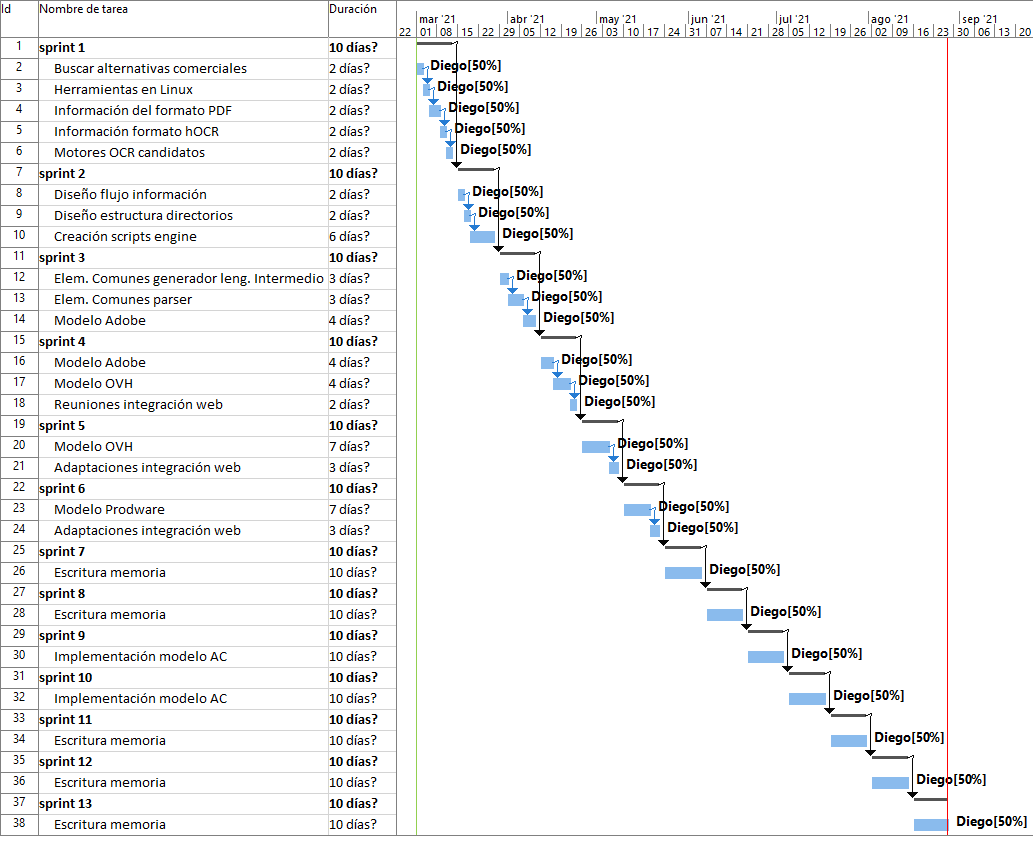
\includegraphics[angle=90,width=1.0\textwidth]{imaxes/f-planificacion/gantt-inicial.png}
    \caption{Diagrama de Gantt y tareas iniciales del proyecto.}
    \label{fig:gantt-inicial}
\end{figure}

\section{Sprints}

Se expone acontinuación la distribución del trabajo a lo largo de los sprints. Por motivos de compatibilidad con el trabajo y responsabilidades personales, se escogió una fórmula de 20 horas de trabajo semanal y una duración de cada sprint de 2 semanas.

\subsection{Sprint 1}

Este primer sprint consistió por completo en un spike con el objetivo de recabar toda la información necesaria para plantear el proyecto a nivel técnico. Algunos de los aspectos sobre los que se adquirió conocimiento fueron:

\begin{itemize}
    \item Alternativas comerciales en la misma temática.
    \item Herramientas y librerías disponibles en Linux para manipular PDF.
    \item Funcionamiento del formato PDF a nivel interno.
    \item Formatos de salida de los motores de OCR, es especial del seleccionado, hOCR.
    \item Posibles engines de OCR candidatos para el proyecto
\end{itemize}

\subsection{Sprint 2}

Con el conocimiento de reunido se procedió a la construcción inicial del sistema para el procesamiento por lotes de los trabajos. Además de diseñar la estructura de directorios utilizada por el proyecto, se crearon el Makefile general, utilizado para las compilaciones y los scripts para implementar el motor.

\subsection{Sprint 3}

En el sprint 3 se crearon las implementaciones inciales del generador de lenguaje intermedio y se preparó el primer parser, que se probó con los documentos de Adobe. Para la construcción de los parsers se deseaba un enfoque modular, que no es habitual en este tipo de herramientas. El objetivo era tener un único programa ejecutable para el parser y un conjunto de plugins que implementarían cada uno un modelo de documento. Dado que este no es el tipo de configuración más habitual, llevó un poco más de tiempo que otros planteamientos más sencillos.

\subsection{Sprint 4}

En este sprint se añadió soporte para la generación de código intermedio y parsing del modelo de OVH. También tuvieron lugar las primeras reuniones de trabajo para explicar el proyecto y decidir las adaptaciones necesarias de cara al prototipo.

\subsection{Sprint 5}

Se completó el modelo de documento del proveedor Prodware. Además se abordaron de forma paralela las tareas relacionadas con el prototipo web. Hubo varias reuniones para facilitar la implemtación de aspectos que no habían sido considerados, como  la necesidad de generar imágenes de las páginas individuales de cada documento, cambio del formato de la marca de tiempo para mejorar la compatibilidad entre sistemas de ficheros y la dockerización de la aplicación.

\subsection{Sprints 6, 7 y 8}

En estas tres semanas se abordó la escritura inicial de la memoria, con la previsión de dejar tiempo al final del proyecto para completarla.

\subsection{Sprint 9}

Implementación de los modelos basados en imagen.

\subsection{Sprint 10}

Implementación de los modelos basados en imagen.

\subsection{Sprint 11}

El sprint 11 se utilizó para construir el prototipo del editor de coordenadas.

\subsection{Sprint 12 y 13}

Los últimos dos sprints se dedicaron a finalizar la escritura de la memoria.


\section{Planificación temporal final}

% TODO explicar que las reuniones se adelantaron a las fechas previstas

 %%%%           %%%%
%%%% ANÁLISIS  %%%%
%%%%           %%%%

\chapter{Análisis}
\label{chap:analisis}

\lettrine{E}{n} este capítulo se tratará los aspectos del análisis de la aplicación. Se verán los requisitos, funcionales y no funcionales, los casos de uso y por último se presentarán los modelos de los documentos tratados.

\section{Actores y casos de uso}

Un caso de uso describe una interacción en entre un rol y el sistema. O cómo es utilizado por un usuario para completar una tarea u alcanzar un objetivo. En el Diagrama \ref{fig:casos-de-uso} se presentan los casos de uso de la aplicación. 

Existen dos actores que interactúan con la aplicación, un Sistema Externo y una Base de Datos:

\begin{itemize}
	\item \textbf{Sistema Externo}: la aplicación está diseñada para comunicarse con el Sistemas Externo mediante invocación directa de comandos o bien un por medio del motor que gestiona el procesamiento. Si bien mediante comandos un usuario podría solicitar la ejecución de trabajos, el objetivo principal es ser un backend en disposición de ser empleado por otros sistemas.
	\item \textbf{Base de Datos}: este agente es consultado para la obtención de datos de identificación de los documentos.
\end{itemize}

Se presentan a continuación los casos de uso de forma detallada:

\begin{itemize}
	\item \textbf{CU-01} - Registrar nuevo trabajo
	\begin{itemize}
		\item \textbf{Descripción}: el Sistema Externo solicita la generación de un nuevo identificador para un trabajo.
		\item \textbf{Precondición}: el motor está operativo y esperando trabajo.
		\item \textbf{Postcondición}: se genera el identificador y se ha creado la ruta correspondiente en el sistema de ficheros para el trabajo.
	\end{itemize}
\item \textbf{CU-02} - Generar JSON
	\begin{itemize}
		\item \textbf{Descripción}: el sistema externo facilita un lote de ficheros y un identificador del trabajo para comenzar su tratamiento.
		\item \textbf{Precondición} el identificador debió ser creado previamente.
		\item \textbf{Postcondición}: los resultados de la operativa están disponibles en las rutas previstas.
\end{itemize}
\item \textbf{CU-03} - Generar imágenes
	\begin{itemize}
		\item \textbf{Descripción}: el sistema genera imágenes para cada una de las páginas de los documentos.
		\item \textbf{Precondición} se han podido recuperar los PDF individuales y se encuentran en las rutas previstas.
		\item \textbf{Postcondición}: existe un fichero para cada página de cada documento en la ruta de salida.
\end{itemize}
\item \textbf{CU-04} - Informar error
	\begin{itemize}
		\item \textbf{Descripción}: en caso de problemas durante el procesamiento se informa al sistema externo del error ocurrido.
		\item \textbf{Precondición} sucede una condición de error en el sistema.
		\item \textbf{Postcondición}: dependiendo del tipo de error el engine consigue finalizar el procesamiento o se finaliza si no es posible recuperarse del error.
\end{itemize}
\item \textbf{CU-05} - Relacionar documento y plantilla
	\begin{itemize}
		\item \textbf{Descripción}: a partir de los datos extraídos del documento en curso se consigue identificar la plantilla correcta para la generación de su lenguaje intermedio y su posterior proceso de parseo. La búsqueda del identificador se solicita a una base de datos externa.
		\item \textbf{Precondición} los datos extraídos son de la suficiente calidad para contener el identificador del documento.
		\item \textbf{Postcondición}: se genera un fichero con el identificador único de la plantilla.Precondición
\end{itemize}
\item \textbf{CU-06} - Identificar la finalización
	\begin{itemize}
		\item \textbf{Descripción}: al finalizar el procesamiento del lote de ficheros se genera una marca de finalización del trabajo.
		\item \textbf{Precondición} se completa el tratamiento de todos los documentos sin errores mayores.
		\item \textbf{Postcondición}: la marca de finalización está en la ruta preestablecida del sistema de ficheros.
\end{itemize}

\end{itemize}

\begin{figure}[hp!]
	\centering
	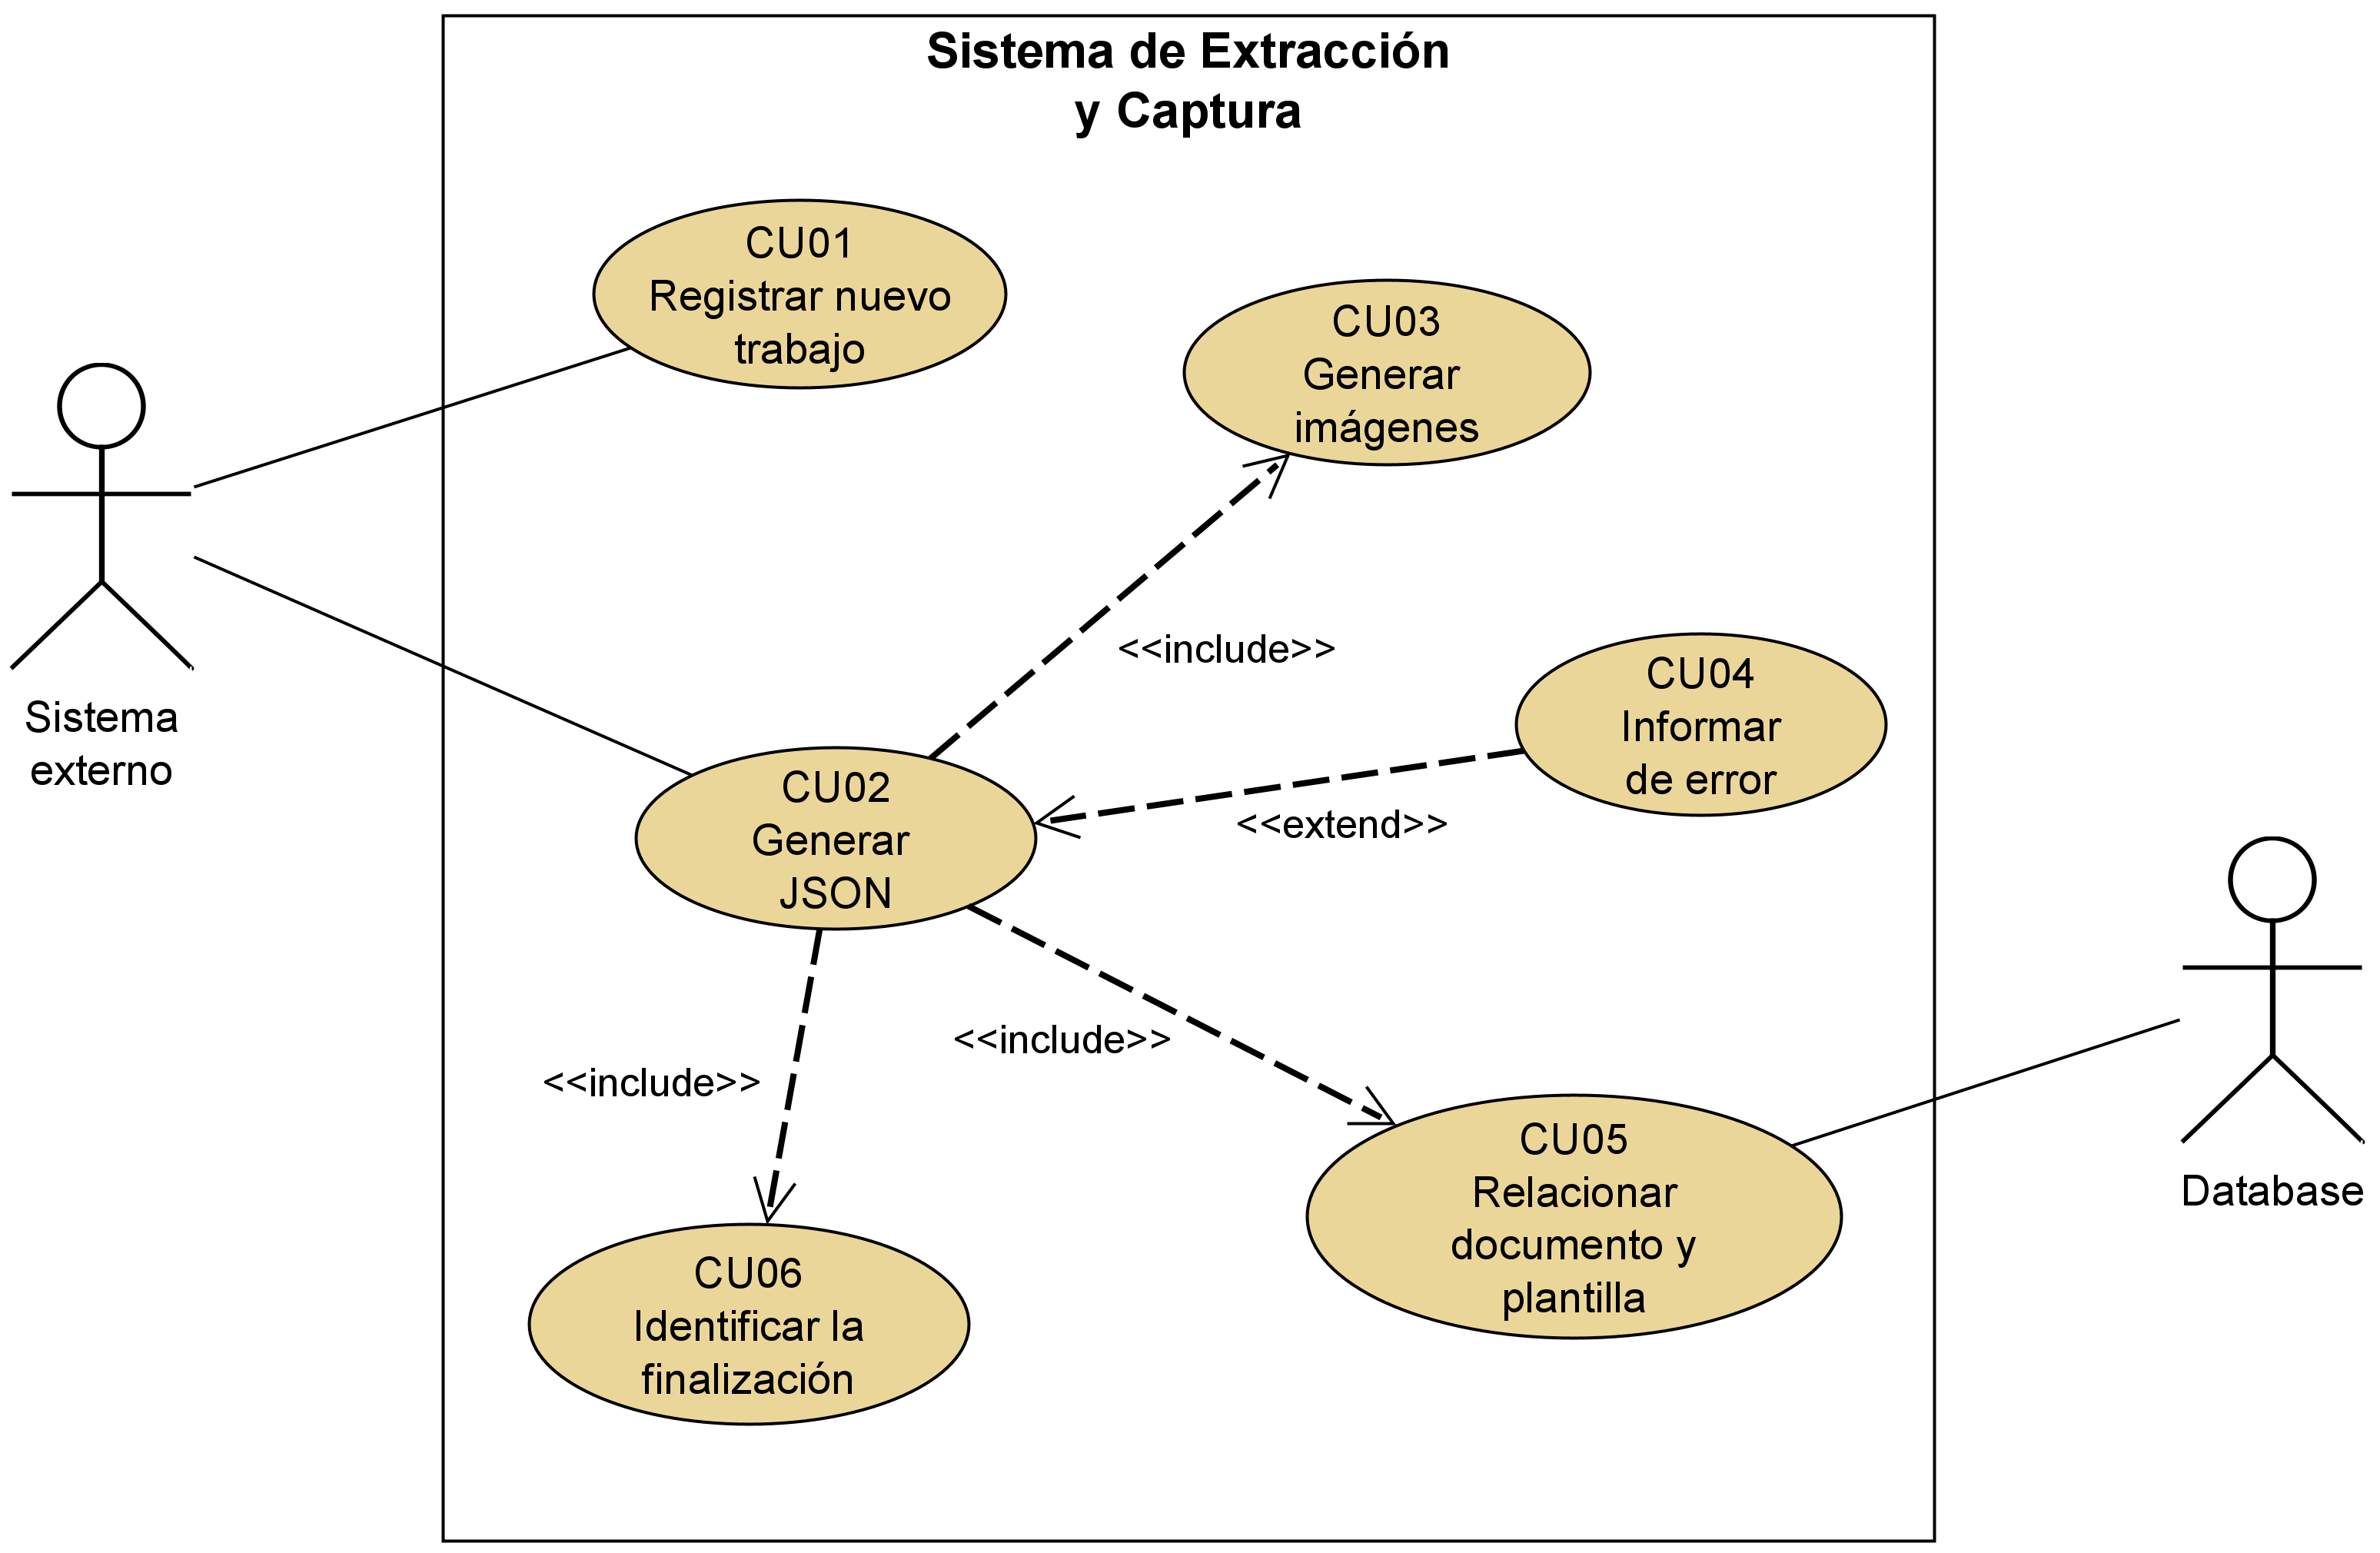
\includegraphics[width=1.0\textwidth]{imaxes/g-analisis/casos-uso.png}
	\caption{Casos de uso del software}
	\label{fig:casos-de-uso}
\end{figure}

\section{Requisitos funcionales}

Estos son los requisitos funcionales que la aplicación debe soportar:

\begin{itemize}
	\item Obtención de un identificador único de un trabajo, con anterioridad a la ejecución del mismo.
	\item Generación una salida en formato estructurado para cada documento suministrado y reconocido en el sistema.
	\item Creación de imágenes de las páginas individuales de cada uno los documentos.
	\item Creación de una marca de finalización para cada trabajo completado.
\end{itemize}


\section{Requisitos no funcionales}

Se exponen ahora los requisitos no funcionales de la aplicación:

\begin{itemize}
	\item La entrada podrá contener uno o más ficheros para su tratamiento en el mismo lote.
	\item Procesamiento de los modelos de imagen y texto de forma transparente al usuario.
	\item La salida de una ejecución debe facilitar los resultados de forma individualizada para cada documento.
	\item Se deben poder identificar las líneas individuales de contenido en  las tablas presentes en los documentos.
\end{itemize}

\section{Sobre los documentos}
\label{sec:sobre-los-documentos}

Para proceder a la inclusión de un nuevo modelo de documento hay entender como está constituido, qué información ofrece, si tienen tablas y como se utilizan en el modelo. En el caso de documentos con más de una página, hay que determinar si en cada una se repiten los mismos elementos o por el contrario, cualquiera de ellas, ya sea la primera, las páginas intermedias o la final, tienen características propias, como puede ser la extensión de las regiones o posición de las mismas. Este análisis de los modelos tratados en el trabajo se presenta a continuación. Para facilitar la compresión de las características se han incluido imágenes completas de algunos documentos en el Apéndice \ref{chap:adicional-1}.

Durante la generación de código y posterior tratamiento del lenguaje intermedio, una de las dificultades habituales consiste en localizar las líneas individuales de contenido. Es frecuente que alguna de las columnas tenga datos en varias filas físicas que refieran a una misma línea de contenido, tal como se muestra en la Imagen \ref{fig:una-linea-lógica-varias-fisicas}. Para un resultado satisfactorio, hay que aprovechar alguna característica que permita esta separación de tal manera que los datos de filas distintas no se mezclen entre si. Esto sucedería si simplemente se generase un código intermedio donde se colocase el texto de forma secuencial considerando únicamente sus coordenadas.

\begin{figure}[hp!]
    \centering
    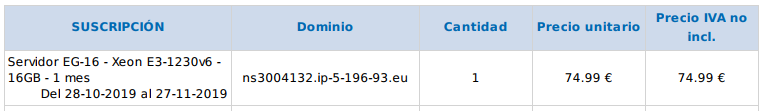
\includegraphics[width=0.9\textwidth]{imaxes/g-analisis/varias-lineas-en-una.png}
    \caption{Una línea lógica utilizando varias líneas físicas}
    \label{fig:una-linea-lógica-varias-fisicas}
\end{figure}

\subsection{Prodware}

Los documentos presentan un layout fijo que se repite en todos los ejemplares. En la parte superior se encuentran los datos de emisor y receptor. Aunque los cuadros no están dibujados, las dimensiones y localización son constantes. Más abajo aparece una primera tabla con una fila para la cabecera y otra fila para la información. La tabla principal de datos tiene tres columnas relativas a la fecha, descripción e importe. En algunos documentos las líneas de la columna \emph{Descripción} ocupan varias líneas físicas. Para la identificación de las líneas de contenido se pueden utilizar las fechas de la primera columna dado que aunque la descripción ocupe varias líneas físicas, las fechas contienen espacios en las segundas o terceras líneas. En la parte inferior están las tablas con información de resumen del documento. Esta información de resumen emplea las mismas dimensiones y espacios en todos los documentos de la muestra. A mayores, dos casos son diferentes en cuanto a que no presentan las líneas de las tablas. No obstante, dado que no es necesario recurrir a la Transformada de Hough para este modelo y que las posiciones se mantienen sin cambios, no supone diferencia para el tratamiento.
 
\subsection{Adobe}

Los ejemplares de facturas de Adobe presentan todos dos páginas. No obstante la segunda página carece de contenido relevante, ya que replica los datos de resumen de la factura, que aparecen idénticos en la primera página. Por tanto las regiones definidas en la plantilla omitirán estas segundas páginas en este modelo.
Todos los casos presentan el mismo layout, con idéntica ubicación para las tablas, celdas y datos individuales. En la parte superior de los documentos aparece la información de identificación del cliente y emisor, a la izquierda, y los datos relativos a la factura, en la parte derecha.
La tabla principal contiene seis columnas. Tras la revisión de los casos no es posible determinar si existen líneas de contenido que se extiendan más allá de una línea física de la tabla.
En la parte inferior se encuentran los datos de resumen como importe, tipo de IVA aplicado y totales.

\subsection{OVH}

Este modelo es el que presenta más variabilidad en su construcción. En la parte superior de la primera página siempre aparece el logotipo de la empresa, a la izquierda, y los datos de identificación de la factura, a la derecha. La información de identificación si que ocupa el mismo tamaño y ubicación en todas las primeras páginas. Para la identificación de las filas de las tablas se utilizará la Transformada de Hough porque existen casos donde el contenido ocupa varias líneas, pero las tablas están perfectamente delimitadas. Por otra parte, las tablas no tienen longitud fija, sino que se extienden tanto como sea necesario para alojar los datos, extendiéndose incluso páginas enteras. Esto quiere decir que no se puede utilizar el tamaño como indicador del final. El interior de las tablas es siempre el mismo. Hay 5 columnas y una primera fila de cabecera con los nombres de las columnas. Encima de la primera fila hay un texto que categoriza la partida de gasto. La última fila de cada tabla contiene la suma del importe de las filas de la tabla precedido de la etiqueta \emph{SUBTOTAL}. Cuando una de las tablas llega hasta el final de la página, siempre se respeta una altura máxima. Esto quiere quiere decir que las regiones se pueden definir utilizando este máximo.

En la última página, si tienen más de una, o en la parte final si solo tienen una, aparece siempre un resumen con los importes. Tras el resumen, existe siempre una línea de texto \emph{Factura pagadera en el momento de la recepción}. La ubicación de esta última tabla puede ser calculada a partir de los textos de la cabecera y de la última línea.

\subsection{AC}

Los documentos de esta empresa pueden tener una o varias páginas. El caso con varias páginas respeta los tamaños y posiciones de los datos. En la parte superior se encuentra el logotipo y datos de la empresa, a la izquierda, y los datos identificativos del cliente, a la derecha. Debajo de la identificación hay regiones simples con los datos identificativos de la factura. En tercer lugar se encuentra la tabla principal de datos que contienen doce columnas. Si bien no se dan casos donde una línea de contenido ocupe más que una línea física, en este modelo algunos datos de columnas diferentes se presentan muy próximos entre si. Aunque el final de la tabla principal no está dibujado, se puede observar que todas las páginas respetan un tamaño máximo que será el punto hasta el que se extienda la región. En la aparte inferior se encuentran los datos de resumen de la factura, con importes desglosados por tipo de IVA y los totales.
 
\subsection{Tipos de regiones}

Vistos los documentos, se concluye que las regiones existentes se pueden categorizar en cuatro tipos y variantes para poder tratar todos los escenarios:

\begin{enumerate}
	\item Tablas simples de dos columnas, cabecera en la columna de la derecha y $m$ filas. Estas son las regiones \verb|R1|, tal como se ejemplifica en la Imagen \ref{fig:region-r1}.
	\item Tablas simples con una cabecera en la primera fila, otra fila de contenido y $n$ columnas. Estas son las regiones \verb|R2|, como en la Imagen \ref{fig:region-r2}.
	\item Celdas individuales, $1\times 1$, donde el contenido se captura de forma secuencial. Estas son las regiones \verb|R3|.
	\item Tablas con $m\times n$ dimensiones y una cabecera en la primera fila. Estas son las tablas con código \verb|T1|.
\end{enumerate}

\begin{figure}
    \centering
    \begin{subfigure}[b]{0.34\textwidth}
        \centering
        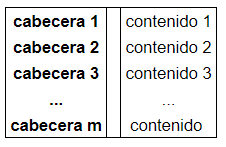
\includegraphics[width=\textwidth]{imaxes/g-analisis/region-r1}
        \caption{Región R1}
        \label{fig:region-r1}
    \end{subfigure}
    \hfill
    \begin{subfigure}[b]{0.65\textwidth}
        \centering
        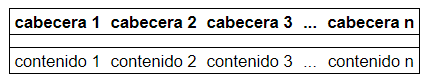
\includegraphics[width=\textwidth]{imaxes/g-analisis/region-r2}
        \caption{Región R2}
        \label{fig:region-r2}
    \end{subfigure}
    \caption{Estructura de dos de los tipos de regiones habituales}
    \label{fig:tipos-de-regiones}
\end{figure}

Una caso especial son las tablas bidimensionales donde se necesita utilizar la Transformada de Hough. Tendrán el código \verb|T2| en las plantillas y por lo demás son similares a las \verb|T1|.

En los documentos de OVH, dado que las tablas no tienen una longitud fija, se consideran en su lugar las relaciones entre las propias tablas y la página en la que se encuentran u otros elementos fijos, como la línea del final, mencionada anteriormente. En las plantillas definirán regiones contiguas, por ejemplo, \verb|T2_T2|. Esto indicará al generador de código intermedio que esta región aplica siempre y cuando se encuentre dos regiones \verb|T2| anexas.

Como conclusión, es de esperar que el tipo de regiones diferentes crezca según se incorporan más y más modelos al sistema. Pero, al mismo tiempo, dado que los tipos de regiones representan un concepto general y son aplicables a cualquier modelo, el objetivo es que su número tienda a estabilizarse con el tiempo.

% TODO aumentar explicación de los tipos de regiones en OVH

\subsection{Características para la identificación}

Para emparejar los documentos con las plantillas que los resuelven se identifican datos específicos presentes en modelos. Dado que todos los casos son facturas, necesariamente aparecerá en ellas el NIF o CIF del emisor. Esta información será suficiente para la identificación. Los mecanismos empleados para realizar el emparejamiento se explican en la Subsección \ref{subsec:impl-identificacion}.


 %%%%                %%%%
%%%% IMPLEMENTACIÓN %%%%
%%%%                %%%%

\chapter{Diseño e Implementación}
\label{chap:implemetación}

\lettrine{E}{ste} capítulo describe el diseño y la implementación de la solución construida. 

\section{Etapas del sistema}

Los datos son sometidos a un proceso por etapas tal como se ve en \ref{vision-general-del-sistema}. A continuación se detalla cada una de estas etapas.

\begin{figure}[hp!]
    \centering
    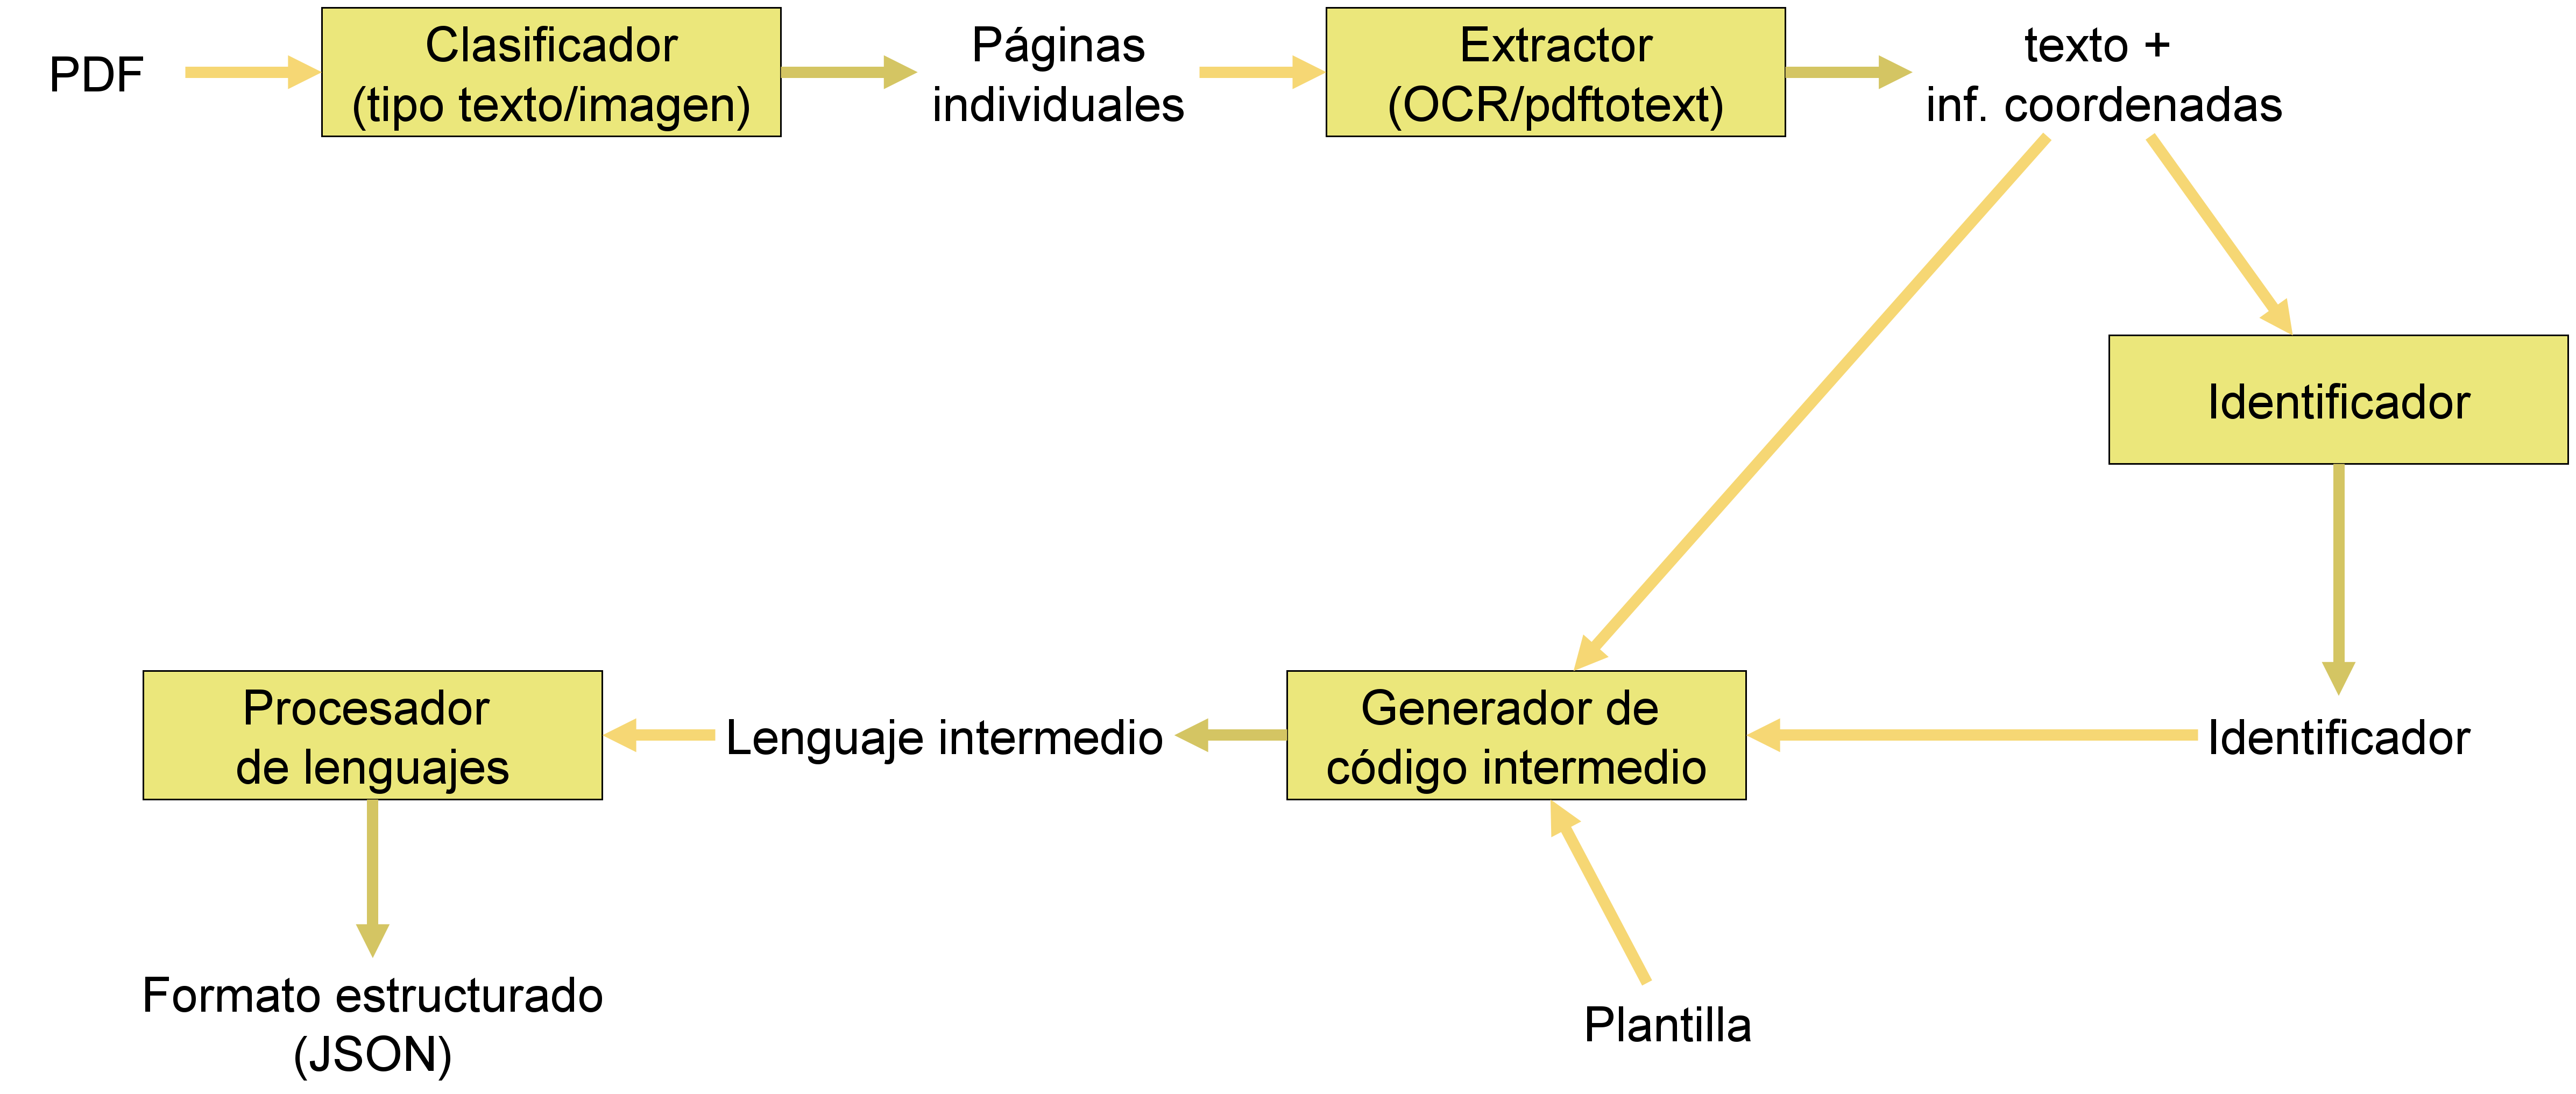
\includegraphics[width=1.0\textwidth]{imaxes/h-implementacion/vision-general-del-sistema}
    \caption{Visión general del sistema}
    \label{fig:vision-general-del-sistema}
\end{figure}

\subsection{Clasificación}

Los PDF recibidos deben ser clasificados dependiendo de su contenido. En unos casos es posible utilizar directamente el texto del documento para los restantes se procederá a utilizar el software OCR.

% TODO explicar en detalle como se hace la diferenciación


\subsection{Extracción de datos}

% TODO separación de las páginas individuales

% TODO comentar caso con pdftotext
% TODO incluir flags utilizados
% TODO ejemplo de salida de la información

% TODO comentar caso con OCR
% TODO parámetros de Tesseract
% TODO para cumplir con el requisito de tiempo reducido de ejecución se configuró Tesseract para emplear todos los cores disponibles en la máquina
% TODO ejemplo de salida de la información

\subsection{Identificación}

% TODO modelo de identificación. Explicar que está pensado para ser extensible a uso de BD u otras fuentes de información
% TODO explicar como se recorre el array en bash
% TODO mostrar la lista de identificadores
% TODO mostrar como se marca el directorio con el fichero .id

\subsection{Plantillas y regiones}
% TODO Tipos de regiones
% TODO información contenida en las plantillas (la que no se refiere a coordenadas)

\subsection{Generación de código intermedio}
% TODO describir la implementación en etapas, como el diagrama general
    % TODO Concepto de línea de identificación
    % TODO Asignación de palabras a regiones
    % TODO información de bounding box
% TODO mostrar el código intermedio
% TODO introducir el problema de indentificar las líneas
% TODO explicar se utiliza el algoritmo de Hough en los ejemplos donde es efectivo
% TODO explicar mejora en el algoritmo para asignación de palabras a regiones para cumplir con el requisito no funcionar de mantener los tiempos contenidos

\subsection{Procesamiento del lenguaje generado}
% TODO explicar como es la estructura general de Flex / Bison
% TODO mostrar las modificaciones introducidas
% TODO explicar la carga dinámica de librerías
% TODO Mencionar que el modelo de plugins permite entregar al cliente solo los modelos comprados
% TODO mostrar como es el formato de un fichero Flex y también Bison
% TODO Mostrar como se utiliza la librería para generación de ficheros JSON
% TODO Mencionar el pretty printing con jq

\subsection{Creación de un engine modular}
% TODO Se imita un modelo de procesamiento en batch
% TODO Se generan códigos de identificación de los jobs recibidos. También marca final.
% TODO Estructura de directorios considerada
% TODO Flujo de la información

\subsection{Compilación y despliegue}
% TODO mostrar el Makefile
% TODO mostrar script Ansible
% TODO Mostrar fichero de configuración Docker y su uso

% TODO valorar si incluir capítulo o sección de pruebas. O, al menos, de pruebas realizadas.

%% La implementación está diseñada para recibir peticiones de conversión y generar la salida correspondiente en formato estructurado. El número de ficheros que se pueden tratar en cada ejecución solo está limitado por las capacidades del sistema de ficheros o del SO donde se ejecute. Cada invocación produce una tarea en el sistema, que se gestiona de forma individual. Una vez que se reciben los ficheros para su tratamiento, se crea una ruta específica para ese trabajo y comienza el proceso. En cada etapa se crean nuevos ficheros intermedios que, según se verá más adelante, se mueven a destinos designados para cada paso. Los documentos se tratan página a página. El motor encargado de conducir el flujo de información está implementado en lenguaje Bash. Este \emph{engine} se apoya en varias herramientas adicionales, disponibles en cualquier distribución Linux. Por último, se complementa con el generador de código intermedio y los \emph{parsers} para cada modelo de documento.

%% Existen, por tanto, tres partes que se detallarán en las siguientes páginas:

%% \begin{itemize}
%%     \item Un motor o \emph{engine} creado con \emph{scripts} en lenguaje Bash. Su cometido es recepcionar los ficheros y transformarlos paso a paso hasta la obtención de la salida final.
%%     \item Una aplicación Python encargada de generar el lenguaje intermedio que va a ser procesado.
%%     \item Una familia de escáners y parsers desarrollados empleando Flex \cite{estes_flex_2021} y GNU Bison \cite{free_software_foundation_inc_bison_nodate}. Toman como entrada el lenguaje intermedio y lo traducen a un formato estructurado.
%% \end{itemize}

%% Se describen a continuación cada una de ellas.

%% \section{El engine}
%% La herramienta se planteó como un software que pudiera ser capaz de recibir uno o varios ficheros en cada invocación. Una vez recibido, cada entrada debía ser clasificada e identificada para su correcto tratamiento. Dado que la entrada y la salida serían ficheros, resultaba natural utilizar un lenguaje de programación con facilidades para la manipulación de ficheros. Por ser el entorno de operación y desarrollo un sistema GNU/Linux, se optó por emplear el intérprete de \emph{shell} Bash.

%% Por tratarse de un conjunto de \emph{scripts}, este \emph{pipeline} es flexible tanto para añadir nuevos pasos como para quitarlos. La razón para hacerlo de este modo radica en posibilitar la incorporación de nuevas técnicas de procesado de cualquiera área relevante, como el tratamiento de imagen o la extracción de texto. Cada \emph{script} es independiente y puede ser ser activado o desactivado fácilmente.

%% Convenio de nombrado para evitar perder información o mezclar páginas

%% Elaboración de las plantillas: Las plantillas son ficheros en formato JSON. Contienen las coordenadas de la geometría para las regiones de interés.

%% Generación del lenguaje intermedio: el sistema de generación de lenguaje intermedio debía ser necesariamente flexible. Para poder aplicar técnicas distintas. Se optó por utilizar Python, que tiene mucho soporte y una gran colección de librerías disponibles.

%% Detección de subregiones: Se diseñó un algoritmo sencillo pero eficaz para decidir si una región era subregión de otra dada.

%% Aproximación para la identificación de las líneas individuales: Esta aproximación se basó en intentar caracterizar las líneas mediante propiedades sencillas. La aproximación no dio resultado.

%% Mejora de tiempos: Inicialmente se utilizada el tipo de dato Set y sus operaciones para comprobar la inclusión de unas regiones en otras. Esta aproximación, aunque funcional, no resultaba rápida para su ejecución durante el desarrollo. Se realizó una mejora que comprueba las propiedades geométricas en lugar de basarse en lógica de conjuntos.

%% Obtención de información estructurada
%%%% Flex
%%%% Bison

%% Despliegue de la aplicación

%% Cambios para integrarse con la GUI
%%%% Exponiendo las coordenadas 
%%%% Uso de Docker

\section{Estructura física}

Para entender más fácilmente las características de la implementación se describen primero la estructura de directorios que conforman el proyecto. 
La estructura y funcionalidad de los directorios del proyecto es importante para entender como se trata la entrada. Esta estructura general se puede consultar gráficamente en XXX. La aplicación se compila y distribuye por medio de un \verb|Makefile|. También existe un fichero \verb|Dockerfile| configurado para generar la correspondiente imagen Docker del programa. Los principales directorios utilizados son:

\begin{itemize}
    \item \verb|conf|, empleado para las configuraciones del \emph{engine}, también la configuración de Tesseract y los datos de entrenamiento.
    \item \verb|data| contiene información de los modelos soportados. Principalmente, los identificadores utilizados para reconocer los documentos y las plantillas que relacionan las regiones seleccionadas.
    \item \verb|doc| está dedicado a la documentación del proyecto. También contiene todos los ejemplos de ficheros PDF utilizados. Esta memoria, escrita con el sistema de composición de textos \LaTeX,  tiene un repositorio de código propio.
    \item \verb|engine| tiene como finalidad alojar todos los \emph{scripts} del \emph{engine}.
    \item \verb|input| no está en el repositorio, sino que se crea bajo demanda. Es la ruta base para la entrada de datos consumidos por la aplicación. El nombre puede cambiarse definiendo otro en la configuración del \emph{engine}.
    \item \verb|script| mantiene varios \emph{scripts} auxiliares utilizados principalmente para facilitar las ejecuciones durante el desarrollo.
    \item \verb|tool-gen-language| es la carpeta dedicada a los fuentes de la herramienta de generación de lenguaje intermedio.
    \item Por último, \verb|tool-parser| contiene la aplicación Flex/Bison y los \verb|plugins| que convierten el lenguaje intermedio a la salida JSON.
\end{itemize}

\section{Tratamiento inicial de la entrada}

La herramienta es un software \verb|backend|, no está pensada para que un usuario realice las ejecuciones de la aplicación manualmente. Por ello, y aunque no se desarrolló un API para acompañar la solución, si que se definieron varias características con la finalidad de facilitar la depuración durante el desarrollo y servir de primera aproximación para una futura integración en un sistema basado en un diseño por capas.

Cada ejecución se realiza en un directorio propio donde se almacena la entrada, se realiza el tratamiento y se ubica la salida. Además, se facilita al programa invocador un identificador que debe utilizar para la recuperación de los resultados. La ruta al directorio que contiene todas las carpetas de todas las ejecuciones el es directorio \verb|input|, mencionado anteriormente.


Para evitar colisiones en las rutas de trabajo entre distintas ejecuciones, se obtiene una marca de tiempo del instante de recepción de la petición y se utiliza como directorio raíz para el nuevo trabajo. Este \emph{timestamp} se obtiene con el comando \verb|date| configurado para generar un entero de tamaño 16 con la hora UTC del sistema: \ref{lst:foo}

\begin{lstlisting}[language=bash,caption={Obtención del identificador del trabajo},label=lst:identificador-trabajo]
    diego@CompaqCQ57:galiasdoc$ date -u +"%s%6N"
    1616623143141490
    diego@CompaqCQ57:galiasdoc$
\end{lstlisting}
%% TODO centrar y añadir caption: ejemplo de directorio de trabajo

A continuación, se presenta la secuencia de pasos que conforman el comienzo de un trabajo. La primera acción ocurre cuando el invocador ejecuta el \emph{script} \verb|get-job-id.sh|. Este crea el nuevo directorio para el trabajo y todos los directorios internos. Se devuelve el identificador de trabajo al programa llamador.

En este momento el llamador debe copiar el fichero de entrada en la ruta \verb|job_id/frontend|. Por último, se inicia la ejecución cuando se llama al \emph{script} \verb|run.sh|. Se le debe indicar al motor el identificador del \emph{job} que se quiere iniciar. Para ello, el \verb|job_id| se pasa como parámetro. Los pasos se pueden seguir visualmente en la figura \ref{fig:inicio-aplicacion}.

A partir de este momento el sistema comienza a trabajar. Cada acción llevada a cabo se indica con un mensaje por la salida estándar de la consola. Cuando finaliza, se notifica con otra marca de tiempo del momento final en la ruta \verb|input/job_id/done-<timestamp>|.

\begin{figure}[hp!]
    \centering
    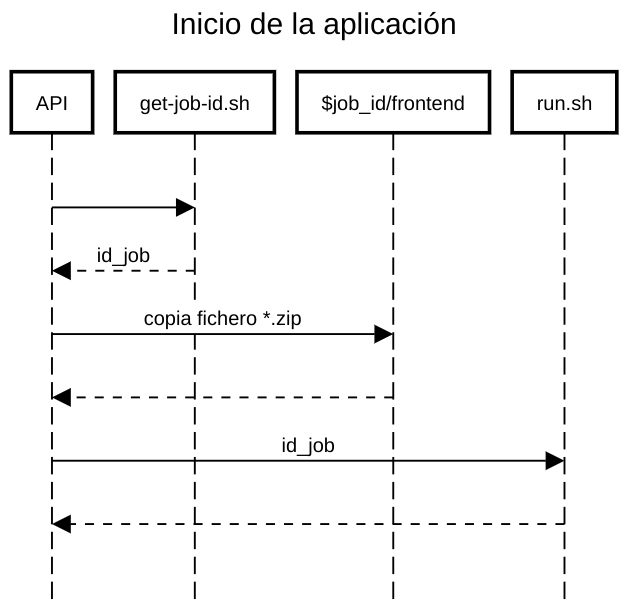
\includegraphics[width=11cm]{imaxes/h-implementacion/inicio-aplicacion.png}
    \caption{Secuencia de inicio de la aplicación}
    \label{fig:inicio-aplicacion}
\end{figure}

%% Cambiar diagrama con flecha saliente para indicar que se ejecutan los pasos del engine
%% Cambiar "copia fichero *.zip" por "datos entrada"
%% La línea de finalización debe devolver el evento de finalización

\section{Flujo de información en el \emph{engine}}

Cuando se invoca el \emph{script} \verb|run.sh| se realizan en secuencia todos los pasos que acaban generado la salida en formato estructurado.

%% Considerar borrado:

%% Primero se descomprimen los datos de entrada y se renombran los ficheros recibidos para que su tratamiento sea seguro al construir las rutas. Seguidamente se realiza una primera extracción de texto con \emph{pdftotext}. En tercer lugar, se realiza una clasificación de los casos basados en texto y aquellos basados en imagen. También se generan imágenes de todas las páginas de los documentos basados en texto. A continuación ya se realiza el Reconocimiento Óptico de Caracteres para los casos %% basados en imagen. Con el OCR completado se trata de identificar cada documento. Lo siguiente es generar el lenguaje intermedio e invocar al \emph{parser} necesario. Por último, se publican los resultados en el directorio de salida del trabajo.

%&

Para facilitar la comunicación, se asume que la entrada llega como un único fichero comprimido. En este primer paso es necesario extraer los contenidos de dicho fichero. Se realiza además un renombrado de cada uno, para evitar errores debidos a caracteres poco amigables con el intérprete de comandos, a la hora de componer las rutas.

Una vez los ficheros PDF ya están disponibles, se realiza una primera extracción de texto con la herramienta \verb|pdftotext|. El objetivo es realizar la clasificación que separe los ficheros de texto de aquellos cuyas páginas son imágenes.

Cuando \verb|pdftotext| en invocado en un PDF sin texto, genera igualmente un fichero de salida cuyo único contenido es un símbolo de fin de página. Por defecto utiliza el carácter \verb|Form Feed| o \verb|0x0D|. Aquellas páginas que dan como resultado únicamente este carácter son movidas al directorio para el tratamiento por imagen, \verb|based-image|.

El siguiente paso consiste en obtener la descripción de las coordenadas de las palabras y las líneas. Para ello \verb|pdftotext| vuelve a ser clave ya que con el flag \verb|-bbox-layout| permite generar un fichero XML que contiene estos datos y también el texto encontrado. Respecto a la calidad del texto hay que tener presente que muchos PDF introducen variaciones en las palabras, típicamente añadiendo espacios entre las letras. Estos problemas son tratados posteriormente.

A continuación se muestra un fragmento de una de estas salidas XML:

\begin{lstlisting}[language=HTML,caption={Obtención del identificador del trabajo},label=lst:salida-pdftotext]
<html>
  <head>
    <title>Factura ES1864857 - OVH</title>
  </head>
  <body>
    <doc>
      <page width="595.000000" height="842.000000">
        <flow>
          <block xMin="1223.064810" yMin="168.431792" xMax="1353.159365" 
              yMax="203.373692">
            <line xMin="1223.064810" yMin="168.431792" xMax="1353.159365" 
                yMax="203.373692">
              <word xMin="1223.064810" yMin="168.431792" xMax="1353.159365" 
                  yMax="203.373692">Factura:</word>
            </line>
          </block>
        </flow>
      </page>
    </doc>
  </body>
</html>
\end{lstlisting}

%% XXX Explicación de representación en coordenadas

Para facilitar a la aplicación gráfica la visualización de los contenidos detectados surgió la necesidad de proporcionar imágenes de las páginas de los documentos de tipo texto. Esto se realiza invocando a la herramienta \verb|pdftocairo|. 

La siguiente fase se extraen contenidos y coordenadas de las páginas con imágenes. En este caso se utiliza Tesseract. Además del fichero de entrenamiento estándar está disponible otro de mayor tamaño y que resulta más certero con un coste temporal mayor. Para los casos tratados los resultados con la versión estándar fueron suficientemente satisfactorios. Todos los ficheros de entrenamiento de la aplicación están disponibles en la web oficial del proyecto XXX. Existe además la posibilidad de %% crear ficheros de entrenamiento propios para casos específicos, el proceso también está documentado en la web oficial XXX. La salida de Tesseract que se utiliza no es simplemente el texto reconocido. Al igual que en el caso de las páginas con texto se necesitan las coordenadas de los elementos encontrados. Esto se consigue con el parámetro \verb|tessedit_create_hocr|. La salida en este caso será un fichero en formato HOCR.

%% XXX Imagen del fichero HOCR abierto con alguna aplicación de visualización

Para poder aplicar la plantilla a un fichero correcta a un fichero determinado es necesario realizar un emparejamiento. En este caso se optó por buscar en los documentos datos específicos que no causaran colisión con otros documentos. Dado que los datos disponibles son facturas de empresas, se optó por utilizar los códigos NIF o DNI del emisor en este caso y que por ley son obligatorios en este tipo de documentos XXX. Se creó un registro con estos códigos y se realiza una búsqueda con %% \verb|grep| sobre los textos extraídos bien con Tesseract bien con \verb|pdftotext|. En los casos tratados esta búsqueda fue lo suficiente robusta.
Cuando un patrón es encontrado, se crea en el directorio donde se está tratando el documento un fichero con el nombre dado al documento en la fase de renombrado y cuyo contenido es el propio identificador encontrado.

\begin{lstlisting}[language=bash,caption={Identificador del documento},label=lst:identificador-documento]
    diego@CompaqCQ57:galiasdoc$ ls input/1617643045714091/based-text/2/*id
    input/1617643045714091/based-text/2/2.id
    diego@CompaqCQ57:galiasdoc$ cat input/1617643045714091/based-text/2/*id
    B83834747
\end{lstlisting}

Llegados a este punto ya está disponible toda la información necesaria para construir la salida. Hay dos \emph{scripts} más que se ejecutan. Primero se invoca a la herramienta de generación de lenguaje intermedio y después al parser Bison correspondiente. El último \emph{script} mueve los resultados al directorio de salida del \emph{job}, donde podrán ser recuperados. Además se crea en la raíz del \emph{job} un fichero vacío cuyo nombre es el \emph{timestamp} del momento finalización de de la %% ejecución.

\section{Generación del lenguaje intermedio}

\subsection{Definiendo regiones con plantillas}

Las plantillas son documentos JSON que contienen toda la información necesaria para localizar el texto de interés del documento. La creación de las plantillas se ha realizado manualmente. En estas plantillas se definen áreas cuadradas o rectangulares donde están las palabras que se desea generar en formato estructurado. Se distinguen cuatro tipos de regiones.

La más sencilla es una región de tipo secuencia, esto es, los contenidos se ordenarán de izquierda a derecha y de arriba a abajo. Después están las tablas simples que contienen una única columna y múltiples filas o viceversa. El último tipo de región son las tablas de datos con nxm filas y columnas. En el interior de cada subregión el texto se ordena siguiendo el mismo procedimiento que en el caso más básico.

%% Para ampliar: más tipos de informaciones recogidos en las plantillas

\subsection{Estructurando la información}

El cometido principal de la herramienta de generación de código intermedio es transformar el texto extraído en un lenguaje con elementos gramaticales que permitan tratarlo con un parser. A partir de las regiones definidas en las plantillas y las coordenadas de las palabras se hace un filtrado. Se descartan todas las palabras que no encajen en ninguna región, las demás se asocian a la región a la que pertenezcan.

Los elementos principales del programa se detallan a continuación:

Primero se tratan los argumentos de entrada. Especialmente se selecciona XXX ¿qué cosas se seleccionan? XXX
Después se realiza el parse de los datos de entrada. Esto transforma la información de coordenadas y los valores de las palabras en estructuras en memoria. Datos que ambos orígenes de datos comparten el formato HTML, es posible utilizar el parser por defecto que proporciona Python, la clase \verb|HTMLParser|, con la finalidad de extraer las líneas y palabras proporcionadas. Se crearon dos clases que especializan la anterior, \verb|xmlTMLParser| y \verb|hocrHTMLParser| para las particularidades %% de cada tipo de origen.

En la aplicación existen tres conceptos distintos de lo que es una línea. La idea más inmediata de una línea es aquella que se aprecia visualmente sobre un documento. Estas son las líneas que querríamos que el sistema identificara como tales. XXX extender concepto de línea con las otras dos ideas. Creo recordar: la línea área que encaja dentro de una columna, pero no se extiende a otras. XXX. Un problema encontrado en esa asignación de palabras a líneas es que hay casos donde una línea abarca %% más de una columna. Para generar correctamente el lenguaje, cada palabra debe pertenecer a una única línea y la línea debe pertenecer a una única columna. Se realiza por tanto un troceado de las líneas excesivamente extensas. Se fraccionan y se asignan a las regiones que les corresponden.

En este punto ya se ha preparado la información para poder llevar a cabo el tratamiento. Se crea en un objeto tipo diccionario que contiene todos los datos conocidos hasta ahora:

\begin{itemize}
    \item Las líneas,
    \item las palabras,
    \item las regiones definidas en las plantillas,
    \item el número de página actual,
    \item el número de páginas que contiene el documento completo,
    \item la ruta a la imagen de la página actual.
\end{itemize}

La penúltima fase asigna contenidos a las regiones definidas en las plantillas y por último se escriben todos los resultados a disco.

\subsection{Tratamiento de las líneas y las regiones}

El objetivo principal en esta fase es asociar a cada región las líneas que le corresponden. Primero se realiza una clasificación de las regiones según apliquen a una única página, por ejemplo la primera o la última; a múltiples páginas o a todas las páginas del documento. Lo que se hace es escoger las regiones que aplican a la página actual atendiendo al número de página que tiene y su posición dentro del documento. Además de los casos básicos mencionados anteriormente, para el correcto %% tratamiento fue necesario implementar comportamientos para las siguientes categorías: 

\begin{itemize}
    \item R1: una región formada por una columna de cabeceras a la izquierda
    \item R2: región con cabecera en la fila superior
    \item R3: región básica con contenidos secuenciales. Se trata como una celda única.
    \item T1: es una tabla bidimensional donde la primera fila contiene la cabecera y tienen múltiples columnas.
    \item T2: similar al caso anterior pero los límites entre las filas de la tabla se calculan por medio de la transformada de Hough.
    \item T2\_T2: configuración de dos regiones T2 consecutivas.
    \item T2\_T2\_R1: región especial formada por una T2\_T2 seguida de otra R1.
\end{itemize}

%% Adentrarse en cómo seleccionan las regiones las líneas que les corresponden.

%% Mostrar tipos de regiones en el apéndice

%% ¿Por qué fue necesario crear las regiones contiguas. Por el documento tipo \emph{papel continuo}. Detallar.

%% Uso de la transformada de Hough para definición de las filas.

\subsection{Creación del lenguaje intermedio}

Por último, los contendidos de cada región se escriben a la ruta de salida. Existe un método para cada tipo de región. Las regiones dobles utilizadas en la fase anterior no se utilizan aquí y solo se trabaja con R1, R2, R3, T1 y T2.

\section{Salida en lenguaje estructurado}

Para crear la salida estructurada a partir del lenguaje intermedio se utilizan las herramientas Flex y Bison. Flex es un generador de escáneres. Flex toma como entrada un conjunto de reglas, expresiones regulares, y es capaz de crear un ejecutable que evalúe una entrada en base a dichas reglas. Bison por su parte es un generador de parsers. Al igual que Flex, Bison transforma un conjunto de reglas gramaticales en un programa ejecutable capaz de evaluar dicha gramática. Cuando trabajan en %% conjunto, Flex envía a Bison los elementos reconocidos, llamados \emph{tokens}, y Bison los evalúa en la gramática.

\subsection{Carga dinámica de escáner y parser}

Para esta herramienta cada modelo de documento equivale a un programa Flex/Bison independiente, que se selecciona dinámicamente al comienzo de la ejecución. El objetivo perseguido con este enfoque es disponer de un único ejecutable capaz de seleccionar la implementación correcta en tiempo de ejecución. A continuación se expone el modelo habitual de construcción seguido en programas Bison y Flex, luego se exponen las modificaciones realizadas para este proyecto.

Un fichero de entrada Flex está dividido típicamente en tres secciones separadas por líneas con los símbolos \verb|\%\%|. La parte de definiciones se utiliza para asignar nombres a expresiones regulares que se pueden utilizar repetidamente y también para definir variables y funciones en C. La segunda sección contiene las reglas. Una regla se forma con una patrón y una acción.

\begin{verbatim}
    \%\{
    Declaraciones globales C
    \}\%
    definiciones
    \%\% 
    reglas
    \%\% 
    código C
\end{verbatim}

De forma parecida, un fichero Bison también está compuesto por tres secciones. La primera sección se utiliza para la declaración de \verb|tokens| y tipos de datos. La segunda sección contiene las reglas, que siguen un formato muy parecido a la notación BNF \footnote{BNF es una notación para reglas gramaticales}. La última sección contiene código C y especialmente es el punto de entrada a la aplicación. En la función \verb|main| se realiza la llamada a \verb|yyparse| dando lugar al comienzo del %% procesamiento de la entrada.

\begin{verbatim}
    \%\{
    /* Declaraciones C globales */
    \%\}
    declaración de tokens
    \%\%
    reglas
    \%\%
    código C. Función main()
\end{verbatim}

% \section{GNU Make}
%
% GNU Make es una herramienta que permite automatizar transformaciones sobre ficheros. \verb|make| es capaz de construir ejecutables a partir del código fuente de un proyecto. Para ello utiliza un fichero \verb|makefile| que contiene todas las reglas necesarias.
%

 %%%%              %%%%
%%%% CONCLUSIONES %%%%
%%%%              %%%%

\chapter{Conclusiones}
\label{chap:conclusiones}

\lettrine{E}{ste} capítulo presenta las conclusiones finales del TFG y algunas líneas de mejora que se pueden acometer en el futuro.

Al comienzo de este proyecto se desconocían muchos aspectos del dominio. Gracias al trabajo realizado, ese conocimiento es ahora más completo y ha permitido crear un software capaz de resolver satisfactoriamente todos los objetivos propuestos en el Capítulo \ref{chap:introduccion}.

De forma general, se ha conseguido realizar la extracción del contenido vía OCR y/o texto. También se ha conseguido filtrar la información presente en los documentos gracias a unas plantillas que delimitan las regiones de interés. La salida creada está estandarizada, tanto en formato como en contenido.

Más concretamente, a partir del estudio de los documentos se ha conseguido identificar regiones equivalentes, aplicables a varios modelos e identificar el tipo de información que contienen.
Esta información se ha concretado en unas plantillas en formato JSON que el sistema toma como criterio para poder operar sobre los datos.
Gracias a la investigación sobre la salida de los sistemas de OCR y la constitución del formato PDF se ha conseguido comprender que la información de coordenadas está disponible y ha podido encontrar un método para explotarla en el trabajo. Se ha creado un software de entorno servidor capaz de procesar lotes de ficheros PDF y crear con ellos una salida ordenada y estructurada. La prueba de su funcionamiento se ha podido hacer con los documentos facilitados para el proyecto. Por último, se ha conseguido adaptar el desarrollo ya realizado para su incorporación con otra aplicación frontend de esta.

\section{Lecciones aprendidas}

El carácter abierto del proyecto, en lo que se refiere a su desarrollo, ha aportado muchas oportunidades para el aprendizaje. Se comentan algunas de ellas:

\begin{itemize}
	\item De forma tardía se descubrió importancia de realizar una historia del arte que permita comprender cuales son las funcionalidades y qué se esperaría de una solución en un entorno real. De otros trabajos existentes se puede aprender como enfocar correctamente un problema, ahorrando mucho trabajo.
	\item En varias ocasiones se planteó la cuestión de donde realizar cierta parte del tratamiento de un modelo, si en el generador de lenguaje intermedio o más adelante en Flex o Bison. Tomar la decisión no siempre es trivial y conlleva comprender mejor como se están repartiendo las responsabilidades en el software.
\end{itemize}

\section{Trabajo futuro}

Llegados a este punto quedan, muchas áreas de posible mejora o refinamiento, como por ejemplo:

\begin{itemize}
	\item Sería de gran utilidad disponer de un asistente para las plantillas. Consistiría en una vista donde se presenta el documento y se pueden seleccionar regiones de forma visual. Al mismo tiempo se podría asignar las caracterizaciones deseadas, como por ejemplo el tipo de región o su aplicación teniendo en cuenta el número de página del documento.
	\item Para reducir los tiempos de procesamiento sería interesante paralelizar las operaciones de extracción de texto y OCR. De forma análoga, la construcción del lenguaje intermedio y el procesamiento del lenguaje son tareas que se pueden realizar de manera simultánea para páginas y documentos diferentes.
\end{itemize}
 

 %%%%%%%%%%%%%%%%%%%%%%%%%%%%%%%%%%%%%%%%
 % Apéndices, glosarios e bibliografía  %
 %%%%%%%%%%%%%%%%%%%%%%%%%%%%%%%%%%%%%%%%

 \appendix
 \appendixpage
 %%%%             %%%%
%%%% ADICIONAL 1 %%%%
%%%%             %%%%

\chapter{Imágenes y código adicional}
\label{chap:adicional-1}

\lettrine{E}{n} este apéndice se presentan imágenes y código adicionales que por su tamaño no se incluyen en el cuerpo de la memoria.

% TODO añadir imágenes de los documentos tratados

\begin{figure}[hp!]
    \centering
    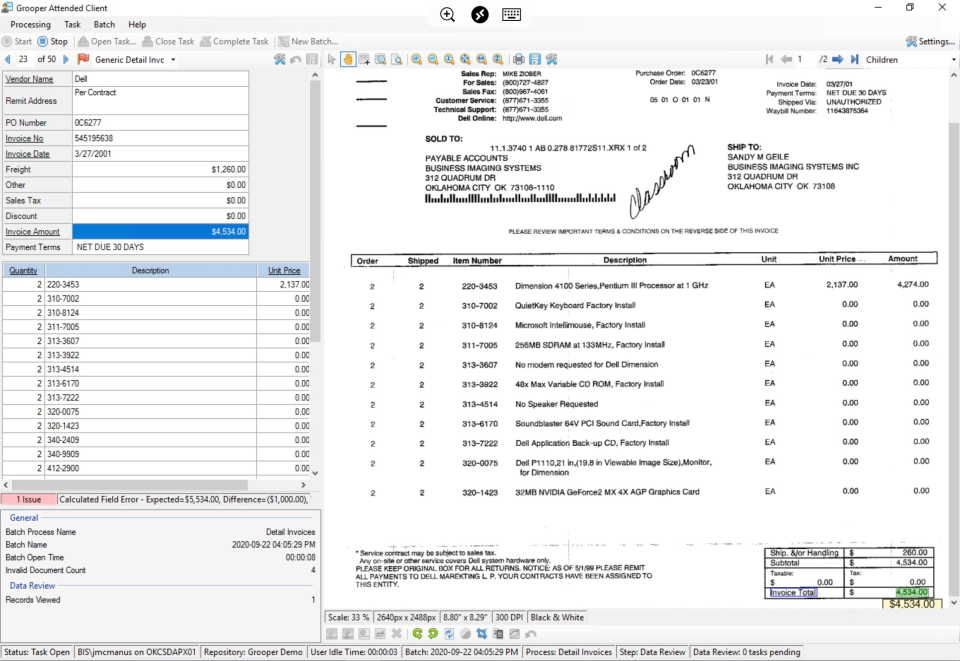
\includegraphics[width=0.9\textwidth]{imaxes/b-estado-arte/bisok-grooper}
    \caption{Grooper, la solución de Bisok}
    \label{fig:grooper-bisok}
\end{figure}

\begin{figure}[hp!]
    \centering
    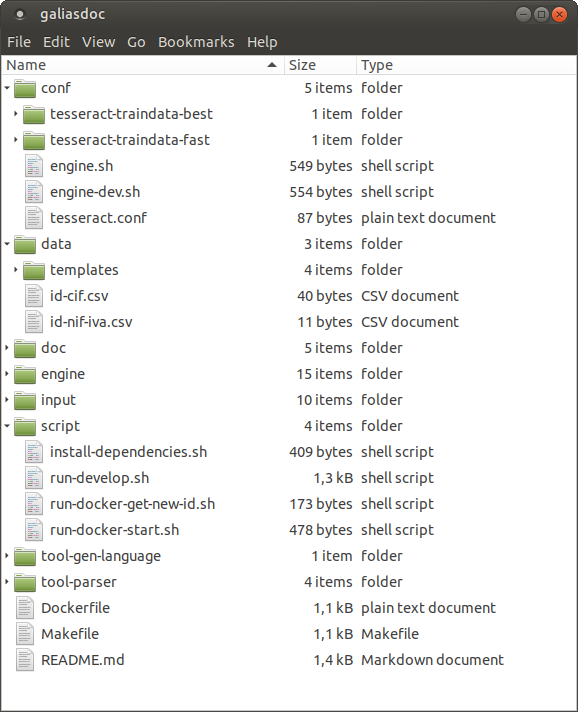
\includegraphics[width=0.8\textwidth]{imaxes/z-adicional/estructura-general.png}
    \caption{Vista general de los directorios del proyecto}
    \label{fig:directorios-proyecto}
\end{figure}

\begin{figure}[hp!]
    \centering
    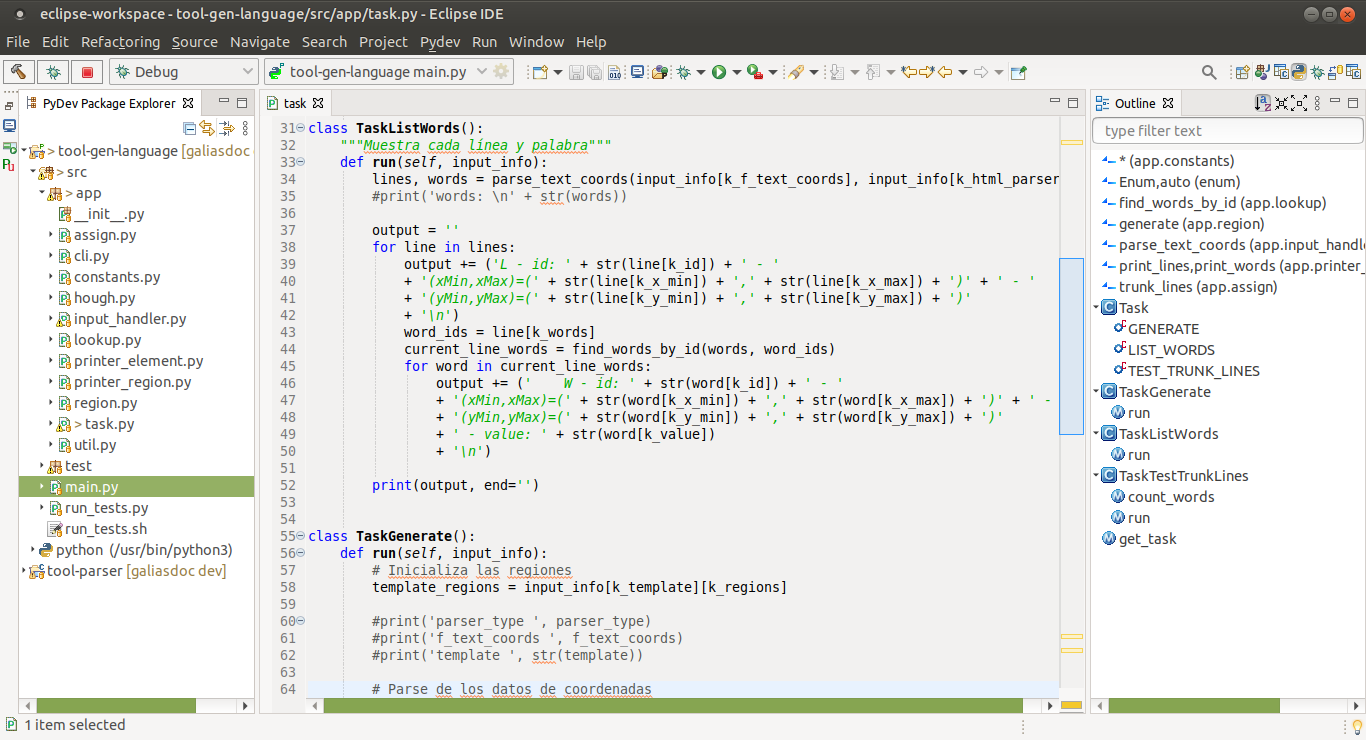
\includegraphics[angle=90,height=1.6\textwidth]{imaxes/z-adicional/tool-gen-language-pydev.png}
    \caption{Eclipse Pydev con el generador de código intermedio}
    \label{fig:tool-gen-language-pydev}
\end{figure}

\noindent\begin{minipage}{.45\textwidth}
\begin{lstlisting}[caption=Scripts del engine]{ScriptsEngine}
engine/
    extract-images.sh
    extract-text-coords.sh
    extract-text.sh
    fix-page-numbers.sh
    generate-images-for-text-based.sh
    generate-json.sh
    get-job-id.sh
    identify-grep.sh
    image-apply-blur.sh
    image-apply-ocr.sh
    image-apply-unskew.sh
    populate-result.sh
    run.sh
    split-text-from-image.sh
    unpack.sh
\end{lstlisting}
\end{minipage}\hfill
\begin{minipage}{.45\textwidth}
\begin{lstlisting}[caption=Fuentes del procesador de lenguaje intermedio,label=lst:fuentes-del-procesador-de-lenguajes]{ProcesadorLenguajes}
tool-parser/
    Makefile
    lib/
        cJSON.c
        cJSON.h
        lista.c
        lista.h
        reg-exp.c
        reg-exp.h
        strbuf.c
        strbuf.h
        util.c
        util.h
    main/
        app-conf.h
        bison-epilogue.c
        bison-epilogue.h
        bison-prologue.c
        bison-prologue.h
        flex-prologue.c
        flex-prologue.h
        gen-amount.c
        gen-amount.h
        gen.c
        gen.h
        global-vars.h
        main.c
        main.h
        types.h
    plugin/
        A48941488.l
        A48941488.y
        B15035801.l
        B15035801.y
        B83834747.l
        B83834747.y
        IE6364992H.l
        IE6364992H.y
\end{lstlisting}
\end{minipage}

\begin{figure}[hp!]
    \centering
    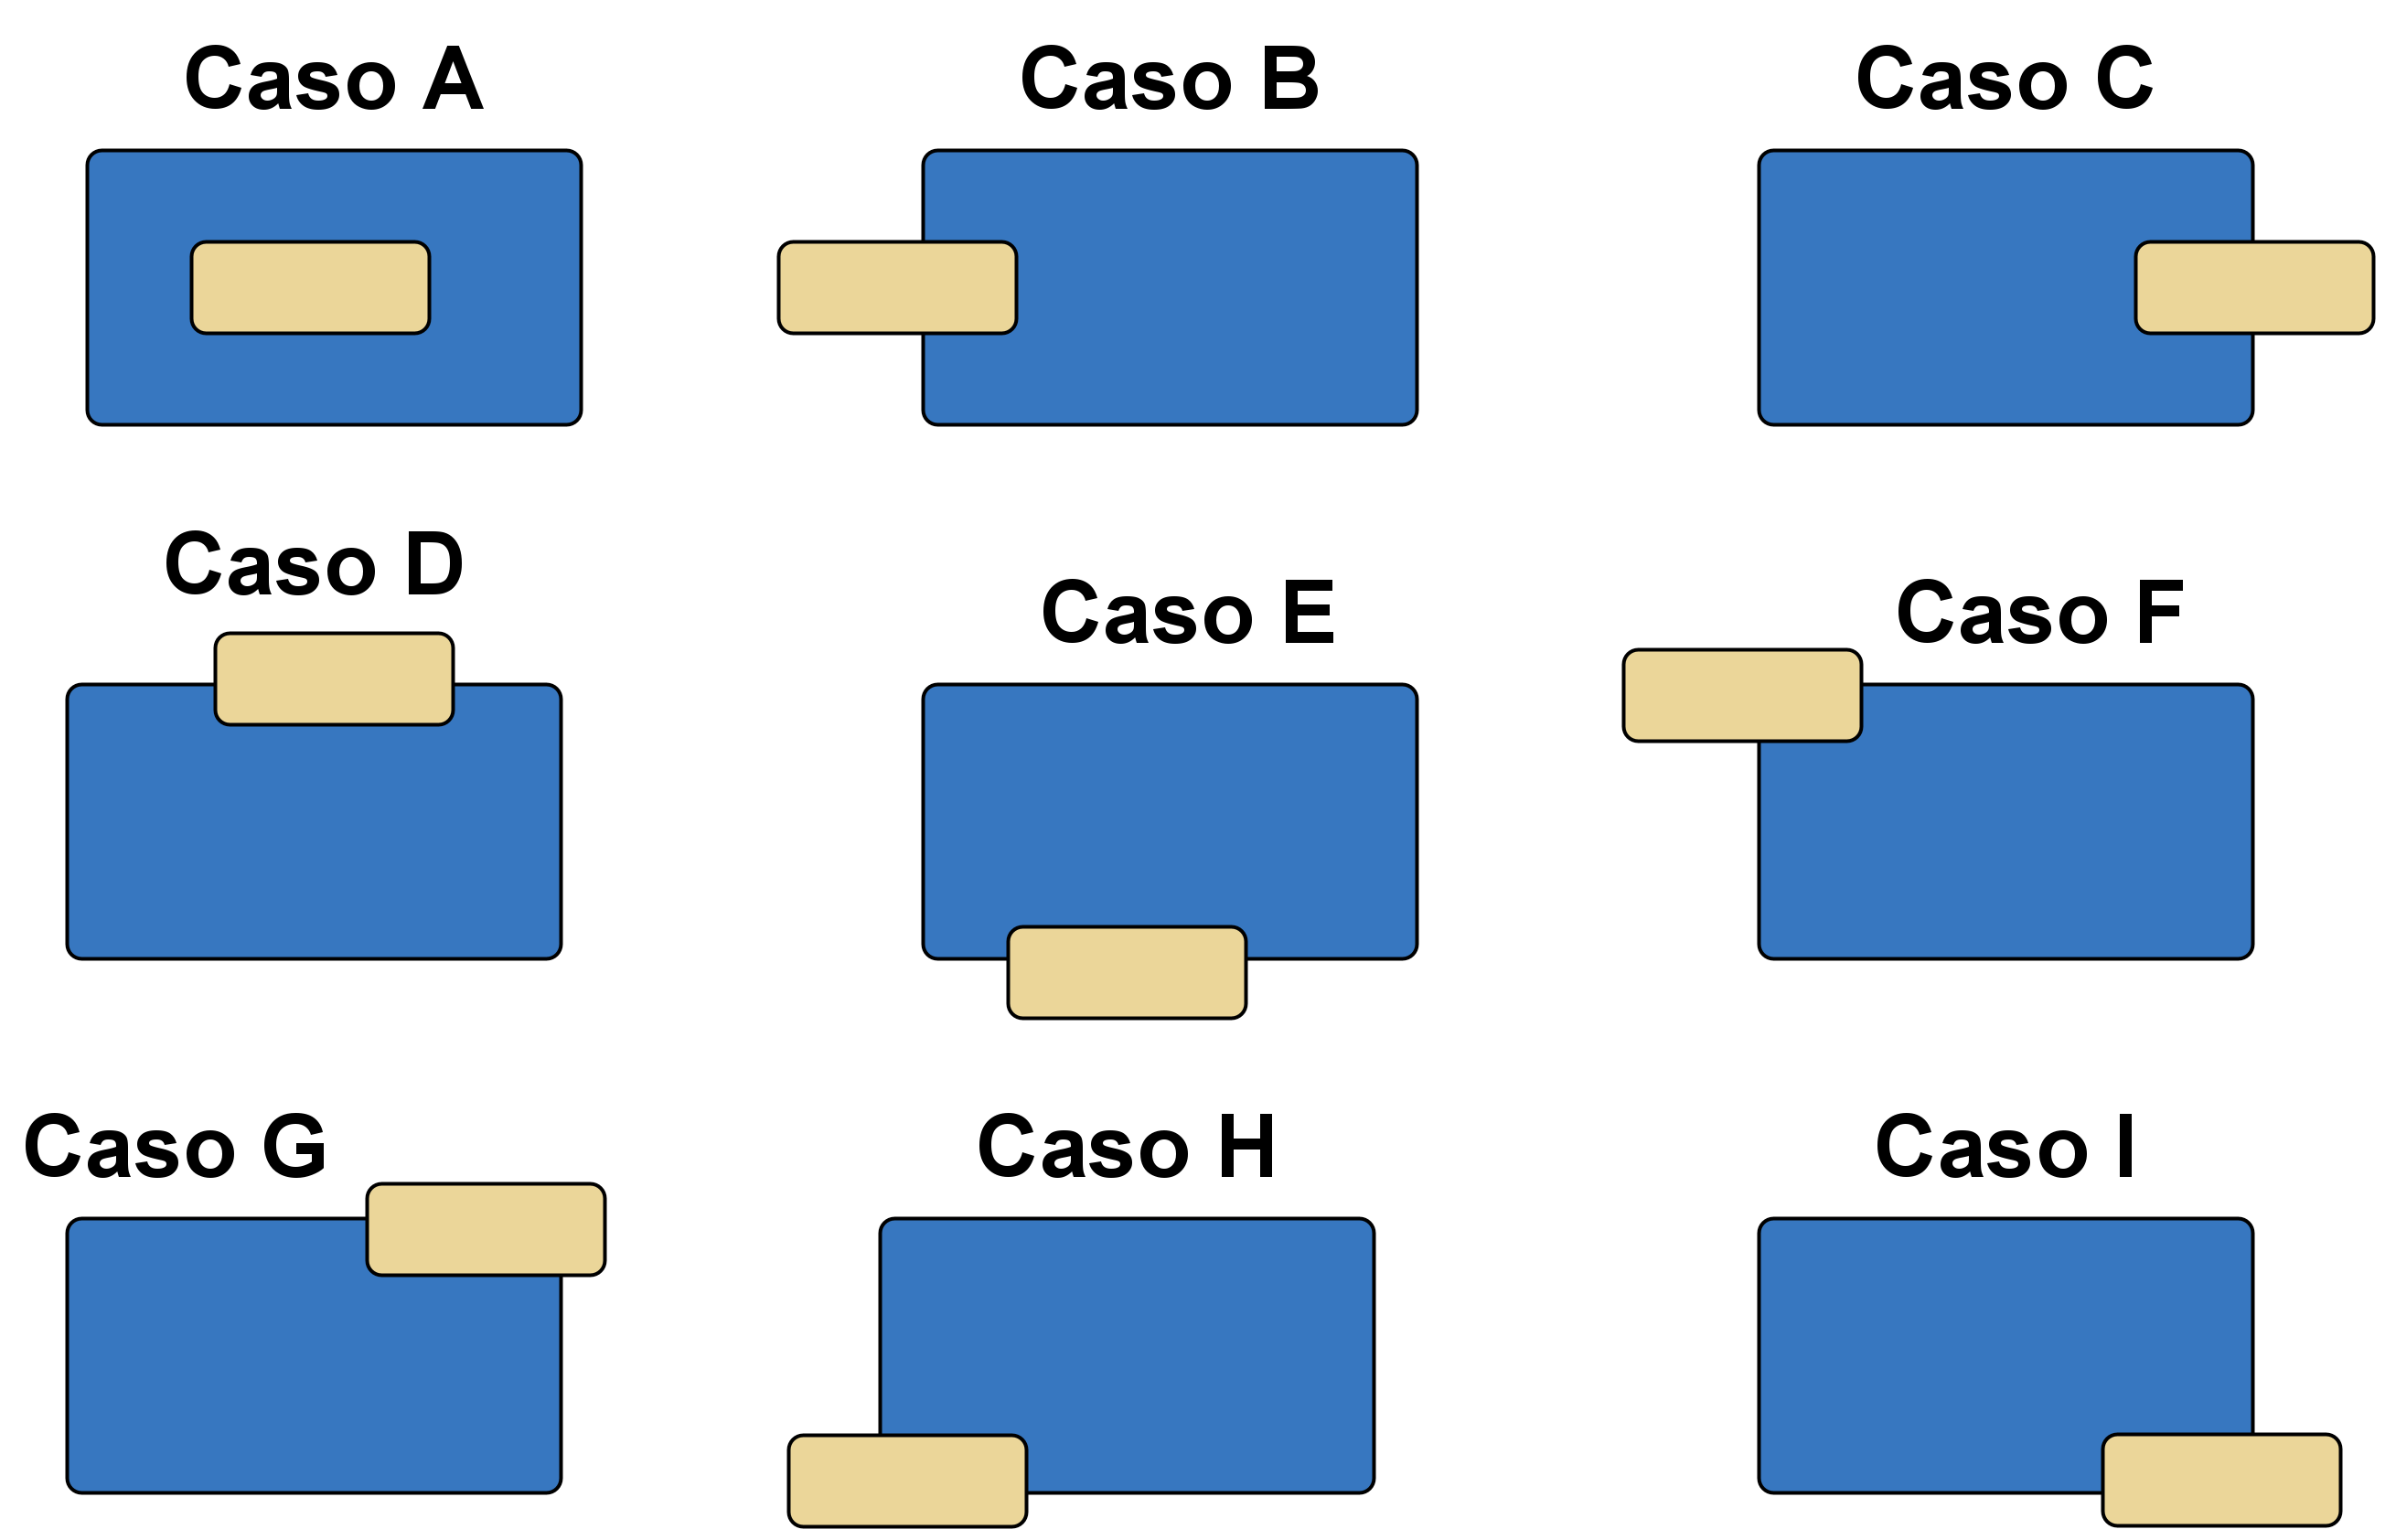
\includegraphics[width=0.8\textwidth]{imaxes/z-adicional/casos-algoritmo-seleccion-regiones.png}
    \caption{Casos considerados en el algoritmo de selección de regiones}
    \label{fig:casos-algoritmo-seleccion-regiones}
\end{figure}

 %%%%             %%%%
%%%% ADICIONAL 2 %%%%
%%%%             %%%%

\chapter{Material adicional}
\label{chap:material-adicional}

\section{Textract y Document AI}
\label{sec:textract-y-document-ai}

Dos servicios diferentes a los productos mencionados en el Capítulo \ref{chap:estado-arte}, pero en un ámbito relacionado con el problema son, Textract de Amazon \cite{solucionesComerciales_amazon_textract} y Document AI de Google \cite{solucionesComerciales_google_documentAI}. Ninguno de los dos soporta el flujo de información explicado, ni están pensados para ser solución para el usuario final. Lo que ofrecen es un \emph{\acrshort{api}} capaz de recibir documentos y generar información estructurada como salida. El caso de Textract es totalmente opaco y por tanto no configurable. La salida consiste en ficheros JSON donde puede haber varios tipos de objetos: páginas, líneas y palabras, información de formularios (en formato par clave-valor), tablas, y elementos seleccionables, como casillas. Además es capaz de identificar notas manuscritas. El servicio de Google permite definir \emph{processors}, que son plantillas específicas para modelos de documentos conocidos. Parece que el servicio es muy reciente y la mayor parte de las funcionalidades publicitadas están en una beta cerrada. Cualquiera de ellos podría utilizarse como parte de una solución más completa. Como otros servicios en la nube, se paga según la cantidad de uso que se hace del servicio o lo que es lo mismo, la carga de trabajo procesada.

\section{Manual de usuario}
\label{sec:instalacion-software}

Se explica seguidamente como proceder a la instalación del software así como realizar la ejecución manual de un conjunto de documentos.

\subsection{Instalación del software}

La instalación completa desde el código fuente implica la descarga del contenido presente en el repositorio git.

En esta sección se asume que se utilizará una distribución Ubuntu 18.04 igual a la empleada durante el desarrollo. Para la correcta compilación y ejecución, es necesario que varias aplicaciones y librerías estén disponibles en el sistema. En el caso de las nuevas versiones de Ubuntu, la lista de paquetes a instalar no presentará diferencias, pero si se utiliza Fedora u otras distribuciones, será necesario averiguar qué paquetes contienen el software utilizado e instalarlos.

Se pueden distinguir dos escenarios distintos. Los requisitos necesarios para compilar los ficheros fuente y aquellos imprescindibles únicamente para ejecutar la aplicación. Para el primer caso se debe utilizar el comando mostrado en \ref{lst:requisitos-para-compilacion}. El paquete \verb|build-essential| instala la mayor parte de las aplicaciones, como el compilador de C y Make.

\begin{lstlisting}[language=bash,caption={Dependencias para la compilación},label=lst:requisitos-para-compilacion]
sudo apt-get build-essential libpcre2-dev bison flex
\end{lstlisting}

En el caso de tener ya la aplicación compilada y empaquetada, será necesarios instalar los componentes para la ejecución, como Tesseract, el software de OCR. La orden del listado \ref{lst:requisitos-para-ejecucion} instalará estos requisitos.

\begin{lstlisting}[language=bash,caption={Dependencias para la ejecución},label=lst:requisitos-para-ejecucion]
sudo apt-get install unzip poppler-utils mediainfo tesseract-ocr tesseract-ocr-spa jq python3-opencv jq bc
\end{lstlisting}

De manera opcional pero recomendable, se puede utilizar un PPA específico para obtener una versión actualizada de Tesseract. Un PPA en el entorno Ubuntu, es un repositorio personal de paquetes listos para su instalación, en este caso mantenido por Alexander Pozdnyakov \footnote{\url{https://launchpad.net/~alex-p/+archive/ubuntu/tesseract-ocr}}. La activación de este repositorio debe hacerse previamente a la instalación del software. Es necesario ejecutar los comandos del listado \ref{lst:activar-ppa-tesseract}.

\begin{lstlisting}[language=bash,caption={Activar PPA de Tesseract},label=lst:activar-ppa-tesseract]
sudo add-apt-repository ppa:alex-p/tesseract-ocr
sudo apt-get update
\end{lstlisting}

\subsection{Ejecución manual}

Para una correcta ejecución totalmente manual, es necesario primero inicializar algunos parámetros de configuración. Se procederá primero leyendo el fichero de configuración que define todas las rutas utilizadas por el \emph{engine}. Así mismo se creará el directorio para los ficheros de entrada:

\begin{lstlisting}[language=bash,caption={},label={}]
conf_file='conf/engine-dev.sh'
source $conf_file
mkdir -p $input_dir
\end{lstlisting}

Acto seguido ya se puede obtener el identificador para un nuevo trabajo:

\begin{lstlisting}[language=bash,caption={},label={}]
job_id=$($app_dir/engine/get-job-id.sh)
\end{lstlisting}

A continuación se copia el fichero comprimido con los documentos a la ruta prevista:

\begin{lstlisting}[language=bash,caption={},label={}]
cp $input_file $input_dir/$job_id/frontend
\end{lstlisting}

Y finalmente se da comienzo al proceso:

\begin{lstlisting}[language=bash,caption={},label={}]
$app_dir/engine/run.sh $job_id
\end{lstlisting}

Al finalizar, los resultados estarán ubicados en \verb|$input_dir/$job_id/frontend|. El \emph{layout} \verb|run-develop.sh| disponible en el directorio \verb|script| realiza de forma automática una ejecución completa con el fichero zip que se le indique por parámetro, como se muestra en la Imagen \ref{fig:ejecucion-manual}

\begin{figure}[hp!]
    \centering
    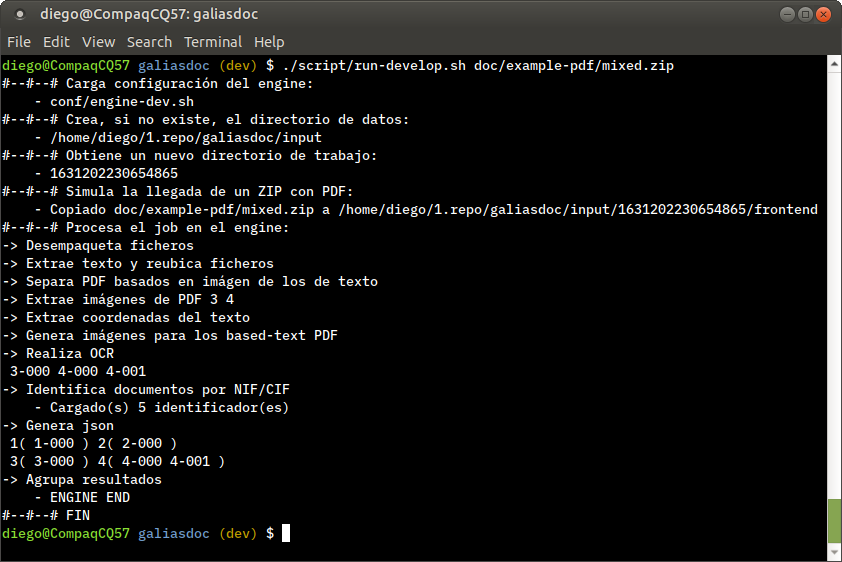
\includegraphics[width=1.0\textwidth]{imaxes/z-adicional/run-develop}
    \caption{Ejecutando manualmente la aplicación}
    \label{fig:ejecucion-manual}
\end{figure}

\section{Visor del formato hOCR}

Existen herramientas para trabajar con el formato hOCR, por ejemplo, las que están disponibles en el repositorio git del proyecto OCRopus \footnote{\url{https://github.com/ocropus/hocr-tools}}. Pero si lo que se quiere es poder visualizar gráficamente como aplican las líneas y regiones de un hOCR sobre una página en particular, el Pattern Recognition \& Image Analysis (PRImA) Research Lab de la Universidad de Salford mantiene una utilidad para hacer justo esto \cite{prima_tool_page_viewer}. En la imagen \ref{fig:visor-formato-hocr}, el visor muestra las líneas detectadas para una página del proveedor AC. Además de hOCR, la herramienta soporta otros formatos, algunos ya mencionados en la memoria como, PAGE XML, ALTO XML o FineReader XML.

\begin{figure}[hp!]
    \centering
    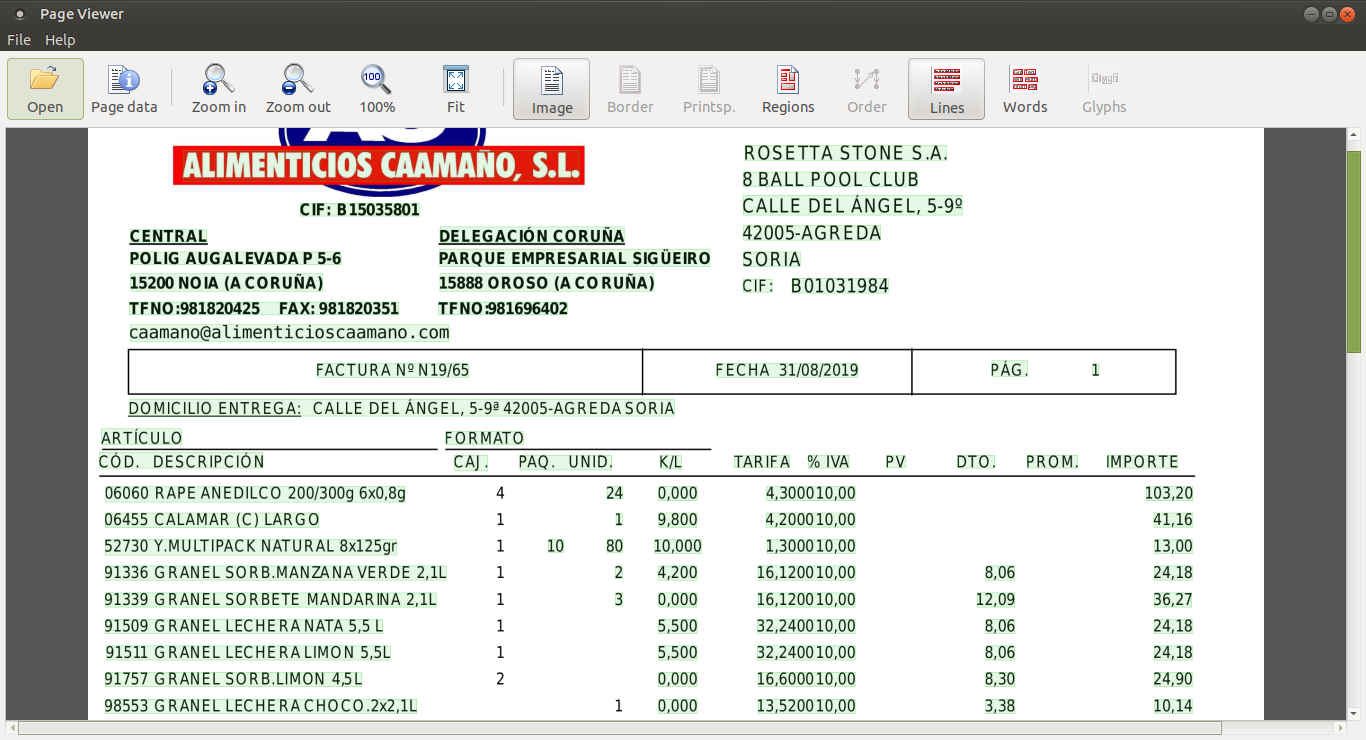
\includegraphics[width=1.0\textwidth]{imaxes/z-adicional/visor-hocr.png}
    \caption{Visor del formato hOCR con un documento de AC}
    \label{fig:visor-formato-hocr}
\end{figure}

\section{Ansible}

% TODO Presentar Ansible y mostrar el script desarrollado

Ansible es una tecnología para automatizar la administración y configuración de ordenadores. Fue creada inicialmente en el año 2012 por Michael DeHaan, hoy en día forma parte del catálogo de productos de Red Hat.

\begin{wrapfigure}{R}{0.3\textwidth}
    \centering
    
\includegraphics[width=0.25\textwidth]{imaxes/e-fundamentos-tecnologicos/logo-ansible.png}
\end{wrapfigure}

Ansible es una tecnología del ámbito de la Gestión de la Configuración. Durante los años 50, el Departamento de Defensa de los Estados Unidos, tenía necesidad de crear una metodología para mantener actualizado el inventario de los recursos materiales disponibles. La Gestión de la Configuración es aquel conjunto de procesos que permiten gestionar los cambios en un sistema, utilizando un método conocido, de tal manera que se mantenga la integridad del sistema a lo largo del tiempo. La manera de lograrlo es manteniendo un registro de los cambios a los que a sido sometido, consiguiendo así conocer cual es el estado actual y como se ha llegado hasta él. Métrica v.3 es un ejemplo de metodología española que incluye la Gestión de la Configuración entre actividades.

Estas ideas se comenzaron a aplicar a los ordenadores para llevar registro tanto del hardware como de los Sistemas Operativos y aplicaciones instaladas. Gracias al avance y aparición de tecnologías como Ansible, en lugar de generar documentos describiendo los estados, se pasa directamente a especificar cuales son los estados deseados y la herramienta realiza los cambios necesarios para asegurar que el estado alcanzado sea el correcto tras la intervención.

Ansible está escrito en Python y su funcionamiento es simple. Para realizar la gestión, conecta a las máquinas mediante el protocolo SSH y aplica los cambios indicados en los ficheros conocidos como Playbooks. Estos ficheros son guiones escritos en lenguaje YAML que indican a Ansible las acciones a acometer. La sintaxis de YAML guarda parecidos con Markdown y es fácil de comprender.

En los Listados \ref{lst:script-ansible-1} y \ref{lst:script-ansible-2} se muestra el Playbook desarrollado para realizar la instalación del software en un servidor remoto.

\noindent\begin{minipage}{.45\textwidth}
	\begin{lstlisting}[language=C,caption={Playbook parte 1},label={lst:script-ansible-1}]{}
---
- name: deploy project to staging
  vars:
    app_dir: solcoerp
    repo_dir: solcoerp-repo
    deploy_dir: deploy
    input_dir: input
  vars_files:
    - svn-credentials.yml
  hosts: backendservers
  remote_user: "{{user}}"
  gather_facts: false
  tasks:
    - name: Remove old deploy directory
      file:
        path: "{{ app_dir }}"
        state: absent
    - name: Check out from repository
      subversion: 
        repo: "{{ repo_url }}"
        dest: "{{ repo_dir }}"
        username: "{{ username }}"
        password: "{{ password }}"
	\end{lstlisting}
\end{minipage}\hfill
\begin{minipage}{.45\textwidth}
	\begin{lstlisting}[language=C,caption={Playbook parte 2},label=lst:script-ansible-2]{}
- name: Call Makefile deploy task
  make:
    chdir: "{{ repo_dir }}"
    target: deploy
- name: Create a root dir for the app 
  file:
    path: "{{ app_dir }}"
    state: directory
- name: Create input directory
  file:
    path: "{{ app_dir  }}/{{ input_dir }}"
    state: directory
- name: Copy deploy dir as app dir 
  copy:
    src: "$HOME/{{ repo_dir }}/{{ deploy_dir }}/"
    dest: "$HOME/{{ app_dir }}/app"
    remote_src: yes 
- name: Remove repo directory
  file:
    path: "{{ repo_dir }}"
    state: absent
	\end{lstlisting}
\end{minipage}



 %%%%%             %%%%
%%%% ADICIONAL 3 %%%%
%%%%             %%%%


  
 \printglossary[type=\acronymtype,title=\nomeglosarioacronimos]
 \printglossary[title=\nomeglosariotermos]

 \bibliographystyle{IEEEtranN}
 \bibliography{\bibconfig,bibliografia/bibliografia}
 \cleardoublepage

\end{document}

%%%%%%%%%%%%%%%%%%%%%%%%%%%%%%%%%%%%%%%%%%%%%%%%%%%%%%%%%%%%%%%%%%%%%%%%%%%%%%%%
